% LuaLaTeX
\documentclass[10pt]{article}

% Packages
\usepackage[no-math]{fontspec}
\usepackage{geometry}
\usepackage{hyperref}
\usepackage[backend=biber]{biblatex} % we use the biber implementation of biblatex for bibliographies
\usepackage[nonumberlist, toc]{glossaries}
\usepackage{graphicx}
\usepackage{pdfpages}
\usepackage{booktabs}
\usepackage{float}
\usepackage{subcaption}
\usepackage{fancyhdr}
\usepackage{amsmath}
\usepackage{siunitx}

% Formatting
\geometry{letterpaper, portrait, margin=.85in}
\defaultfontfeatures{Ligatures=TeX}
\setmainfont[
    BoldFont       = Avenir Medium,
    ItalicFont     = Avenir Book Oblique,
    BoldItalicFont = Avenir Medium Oblique
]{Avenir Book}
\setmonofont{Andale Mono}
\sisetup{detect-all} % used by siunitx to always typeset units in the font of the current environment
\urlstyle{same}

\newcommand\theteamname{Midnight Sun Solar Car Team} % should not change normally
\newcommand\theuniversityname{University of Waterloo} % should also not change normally
\newcommand\theteamwebsite{www.uwmidsun.com} % should also not normally change
\newcommand\theteamphone{(519) 888-4567 x32978} % should also not normally change

\newcommand\thetitle{Preliminary Vehicle Design Report} % <--------------- add the title
\newcommand\thesubtitle{Mechanical} % <--------------- add a subtitle or leave the field empty
\newcommand\theauthor{Minghao Ji} % <--------------- add an author with contact info or leave the field empty
\newcommand\theauthorcontact{minghao.ji@uwmidsun.com} % <--------------- add author's email or leave the field empty
\newcommand\thedate{October 15, 2017} % <--------------- update the date, use this format

\pagestyle{fancy}
\renewcommand{\headrulewidth}{0pt}
\lhead{\thetitle}
\rhead{\theteamname}

\begin{document}
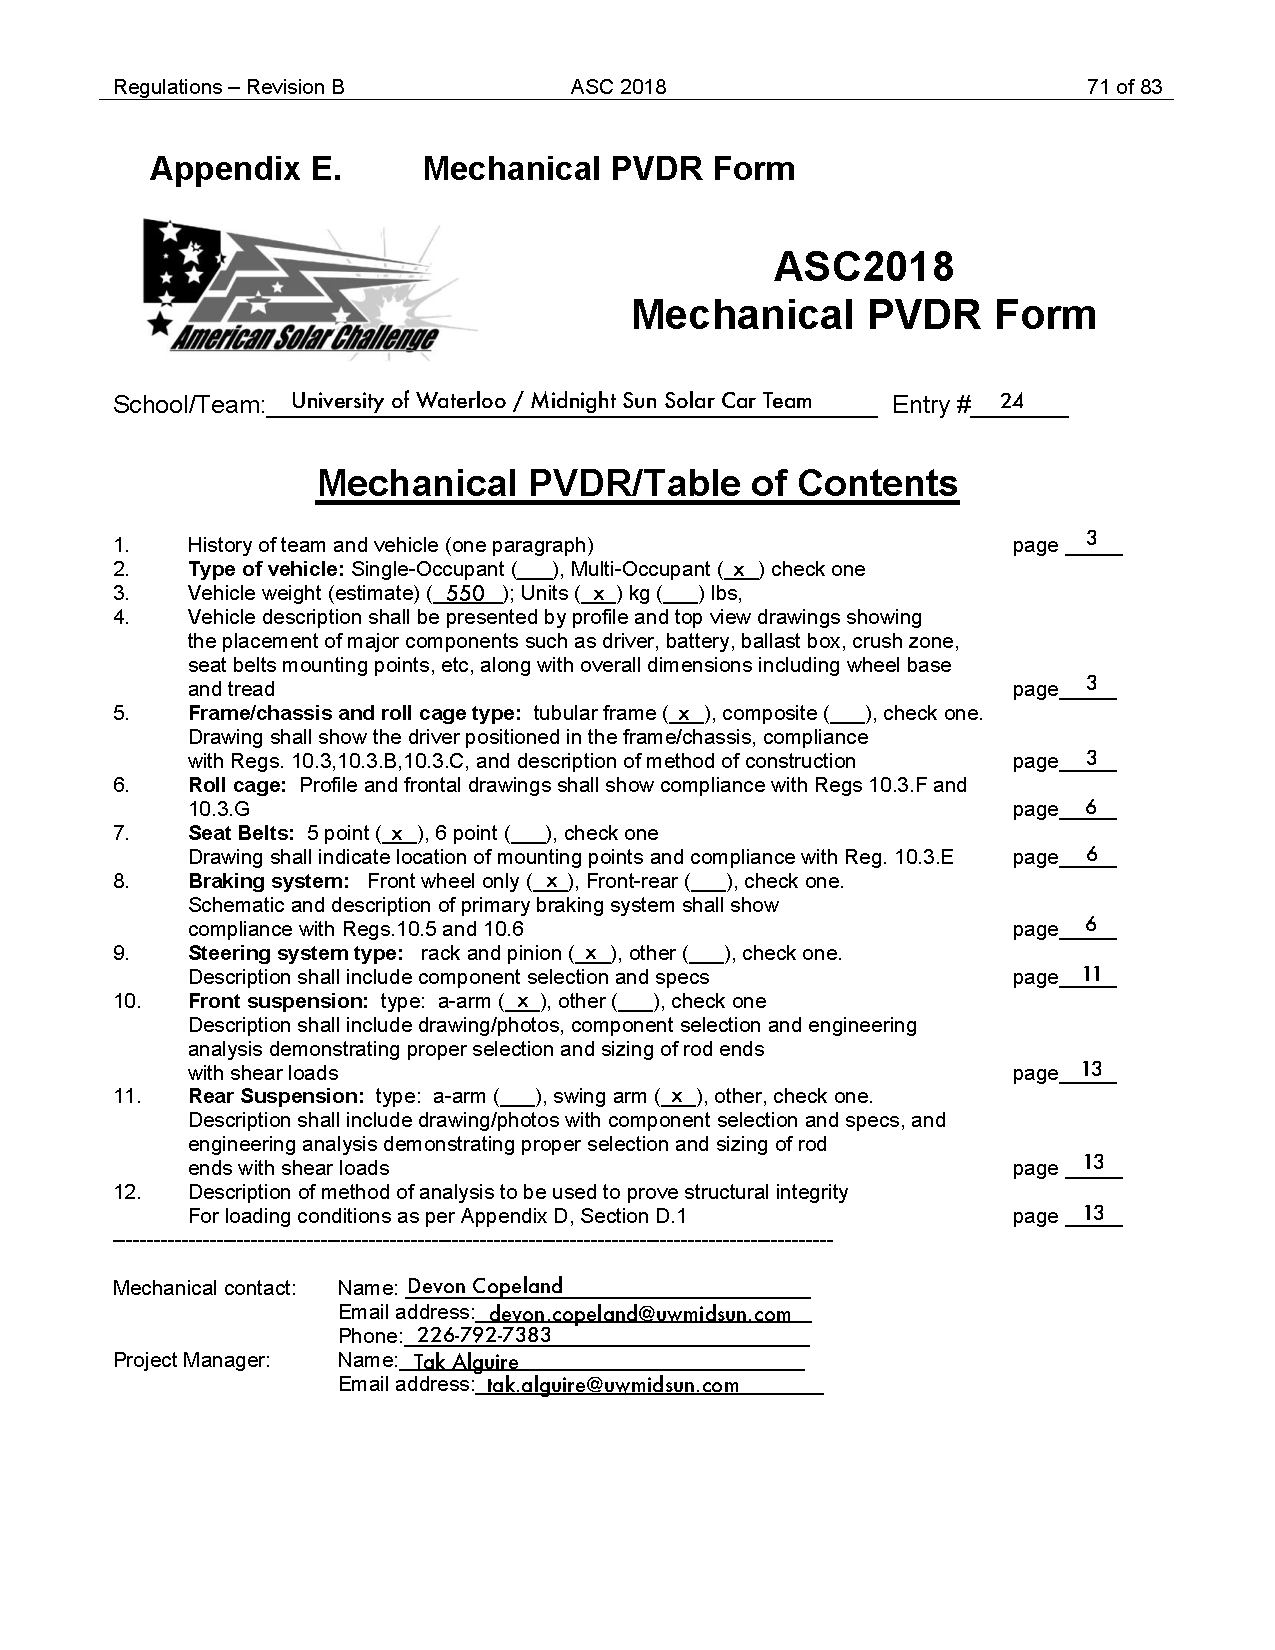
\includepdf[pages={-}]{forms/cover_page_flattened.pdf}

% Title Page
\begin{titlepage}
\large
\vspace*{2cm}
\centering

\includegraphics[width=.25\textwidth]{figures/midnightSunLogoCircle.png} \\
\vspace{1.5cm}
{\LARGE \theteamname} \\
\theuniversityname \\
\vspace{2.2cm}
{\LARGE MSXII} \\
\vspace{0.4cm}
{\huge\bfseries \thetitle} \\
\vspace{0.2cm}
{\LARGE \thesubtitle} \\
\vspace{2.2cm}
\ifdefined \theauthor
\par Prepared by: \\
\theauthor \\
\theauthorcontact \\
\fi
\thedate \\
\vfill
\theteamwebsite \\
\theteamphone
\end{titlepage}

% Main Matter
\tableofcontents
\listoffigures % <-------------- uncomment for list of figures
\listoftables % <-------------- uncomment for list of tables

\section{History}
Midnight Sun was founded in 1988 at the University of Waterloo. The team has produced 11 solar-powered vehicles since its inception, numbered MSI through MSXI. MSX and its predecessors have been traditional Challenger class cars. MSXI was the team's first attempt at a Cruiser class vehicle, which ultimately suffered from design issues relating to its monocoque design. With MSXII, the team has regrouped and designed a new Cruiser vehicle from the gound up, focussing strongly on reliability, safety, and manufacturability.

\section{Contacts}
Questions regarding the mechanical design and implementation of MSXII should be directed to one of the following contacts:

\begin{table}[!h]
\centering
\begin{tabular}{llll}
\toprule
Name            & Title               & Phone        & Email \\
\midrule
Tak Alguire     & Project Manager     & 519-574-4610 & tak.alguire@uwmidsun.com \\
Minghao Ji      & Engineering Manager & 519-500-1292 & minghao.ji@uwmidsun.com \\
Devon Copeland  & Mechanical Lead     & 226-792-7383 & devon.copeland@uwmidsun.com \\
\bottomrule
\end{tabular}
\end{table}

\section{Overview}
MSXII is a dual-occupant Cruiser class vehicle. Its structural design uses a steel alloy tube chassis with non-structural fibreglass body panels. The majority of the vehicle's powertrain systems are located behind the occupant cell, including the battery pack, power junction box, motor controllers, and EV charger. The vehicle is rear-wheel driven by two hub-mounted DC motors. The locations of these components are marked in Figure \ref{fig:msxii-top-view-annotated} and Figure \ref{fig:msxii-side-view-annotated}. Major vehicle dimensions are summarized in Table \ref{tab:msxii-dimensions}.

\begin{figure}
\centering
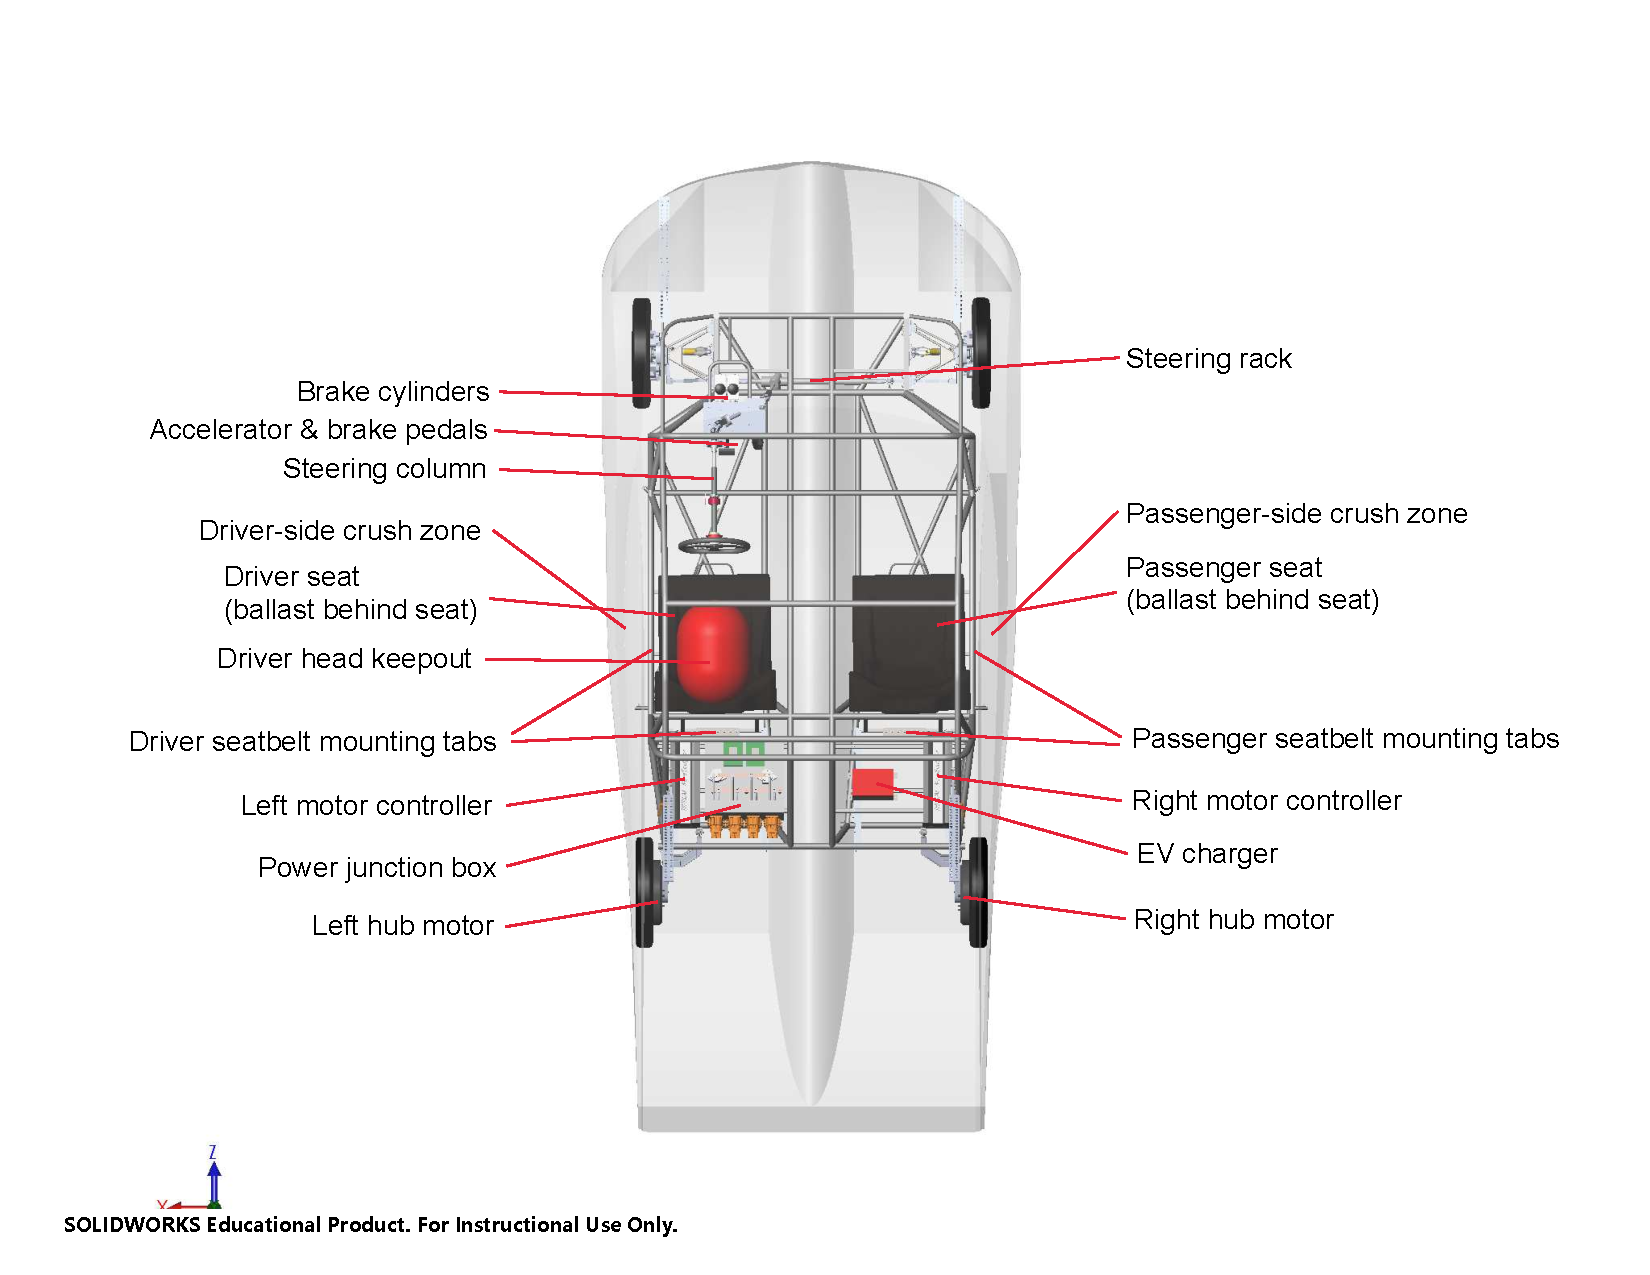
\includegraphics[width=\textwidth]{figures/msxii-top-view-annotated}
\caption{Top view showing major dimensions and system positions}
\label{fig:msxii-top-view-annotated}
\end{figure}

\begin{figure}
\centering
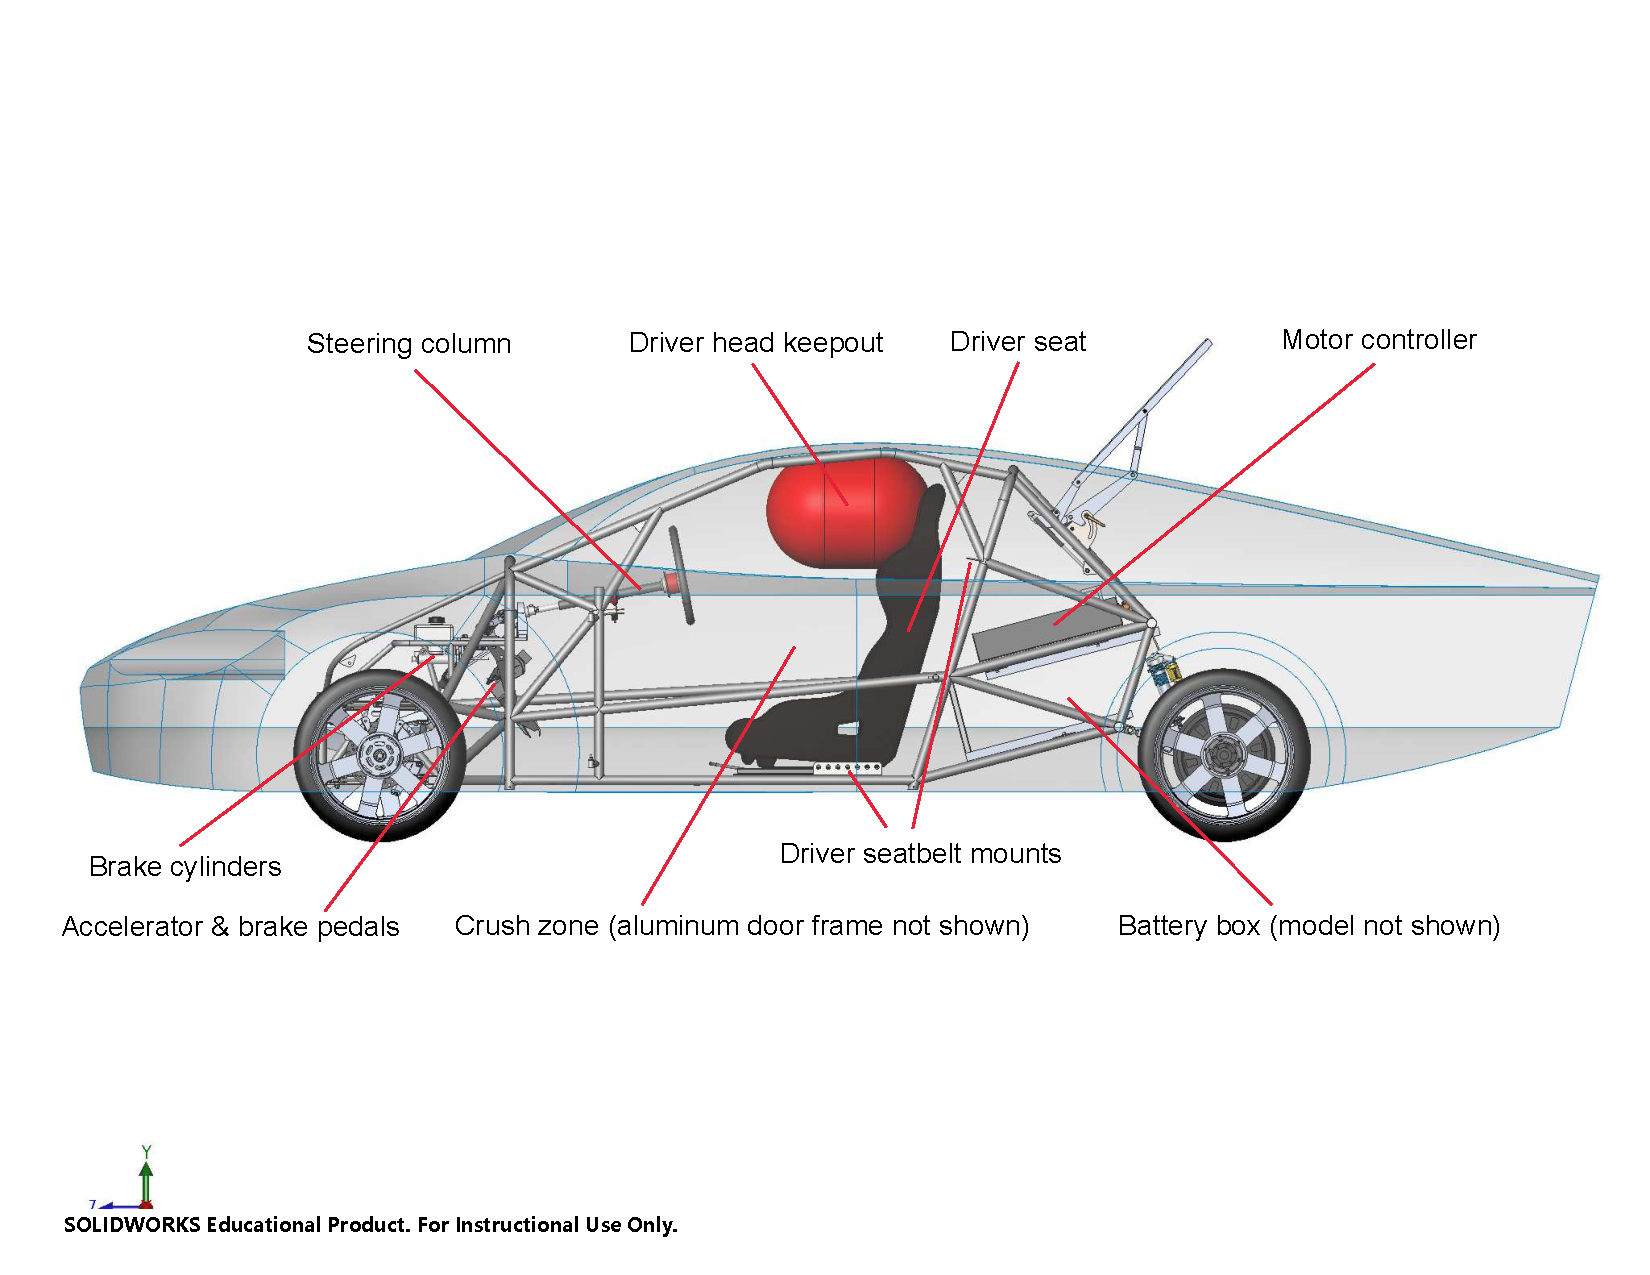
\includegraphics[width=\textwidth]{figures/msxii-side-view-annotated}
\caption{Side view showing major dimensions and system positions}
\label{fig:msxii-side-view-annotated}
\end{figure}

\begin{table}
\centering
\begin{tabular}{cc}
\toprule
Wheelbase    & \SI{2.60}{\metre}    \\
Track        & \SI{1.60}{\metre}    \\
Max length   & \SI{4.68}{\metre}    \\
Max width    & \SI{2.02}{\metre}    \\
Max height   & \SI{1.23}{\metre}    \\
\bottomrule
\end{tabular}
\caption{Table of major vehicle dimensions}
\label{tab:msxii-dimensions}
\end{table}

\section{Chassis}
\subsection{Design}
The chassis is a tube structure enclosing the occupant cell with small front and rear subframes to support suspension hardpoints. Smaller non-structural tube members will extend from the main frame to provide support to body panels as necessary. The majority of tubes are round, with square tubes being used only for elements intended to mount suspension and powertrain components (battery pack, motor controllers). Chassis elements use SAE 4130N chromoly tubes with diameters or side lengths ranging from 0.750" to 1.250", and wall thicknesses ranging from 0.035" to 0.065". Isometric drawings of the chassis are shown in Figures \ref{fig:chassis-front}, \ref{fig:chassis-top}, and \ref{fig:chassis-side}.

\begin{figure}
\centering
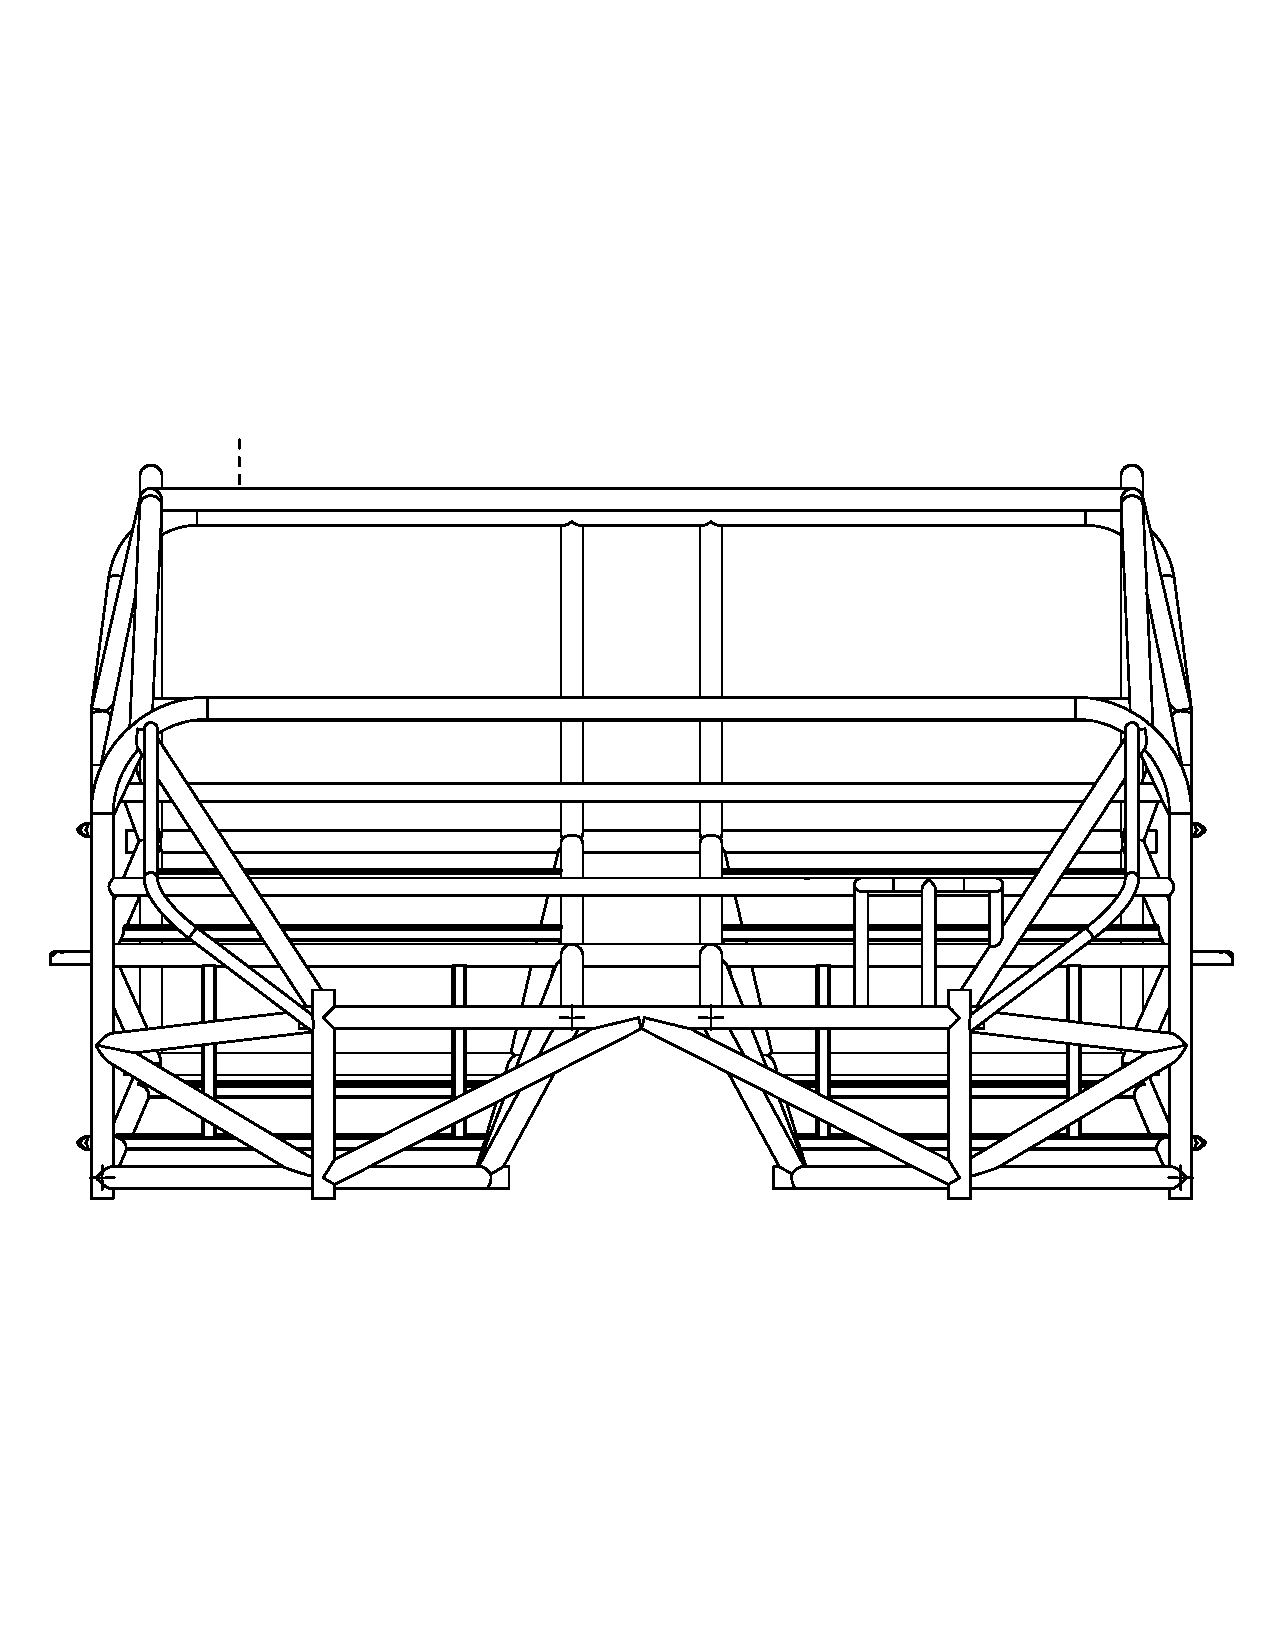
\includegraphics[width=0.75\textwidth]{figures/chassis-front}
\caption{Chassis, front view}
\label{fig:chassis-front}
\end{figure}

\begin{figure}
\centering
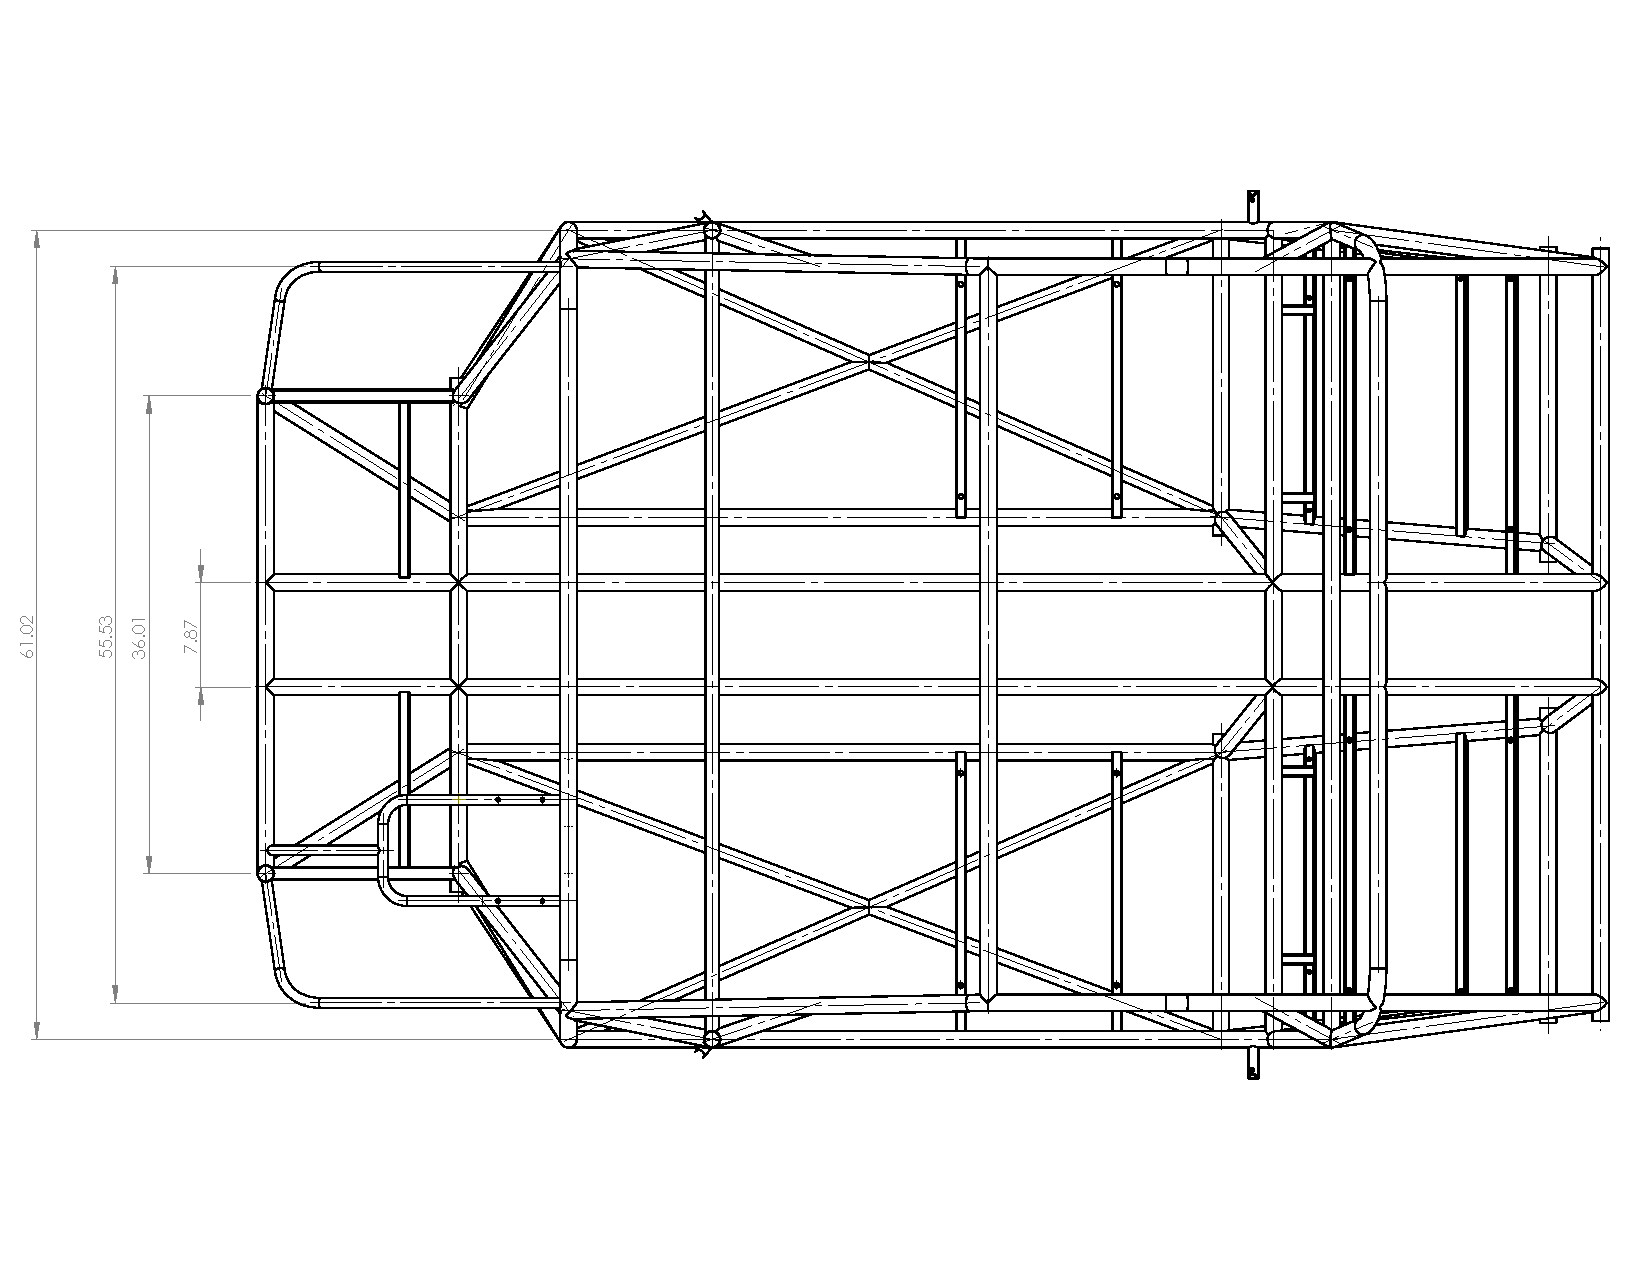
\includegraphics[width=0.9\textwidth]{figures/chassis-top}
\caption{Chassis, top view}
\label{fig:chassis-top}
\end{figure}

\begin{figure}
\centering
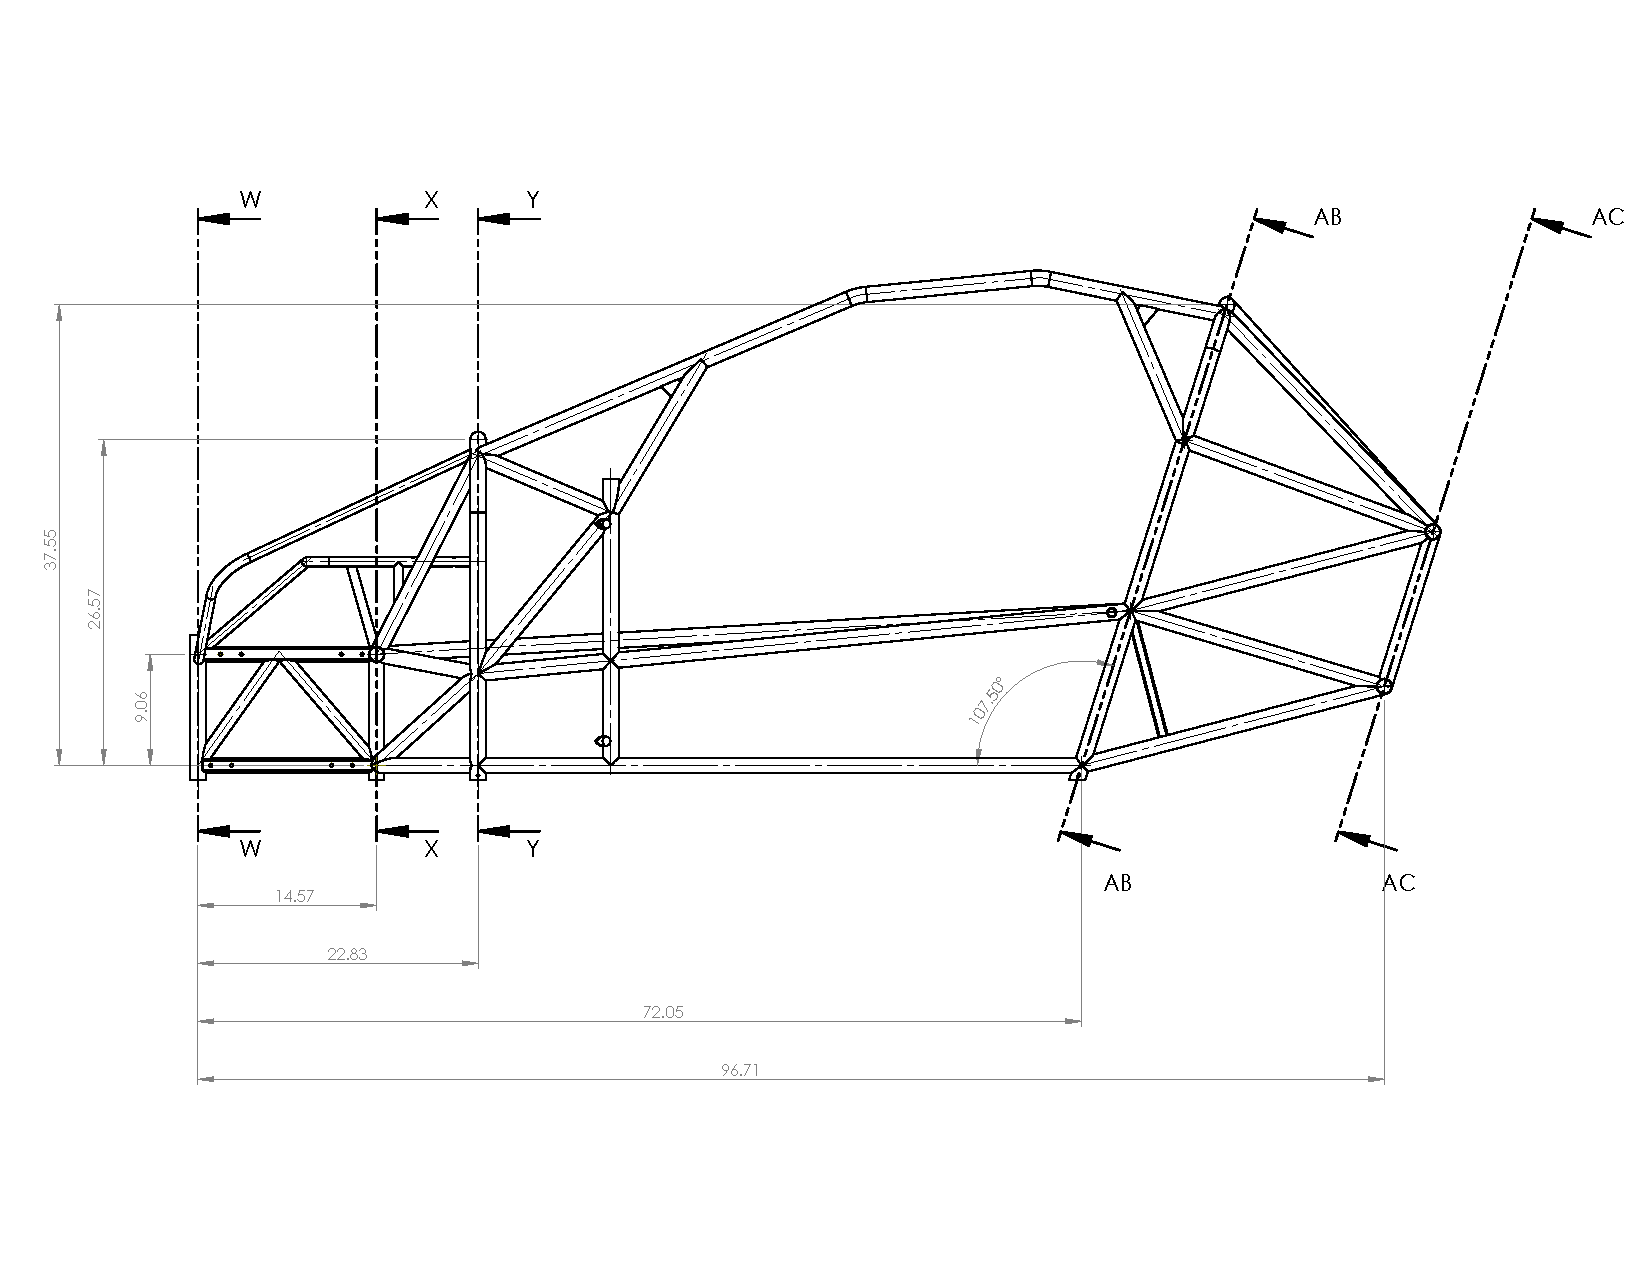
\includegraphics[width=\textwidth]{figures/chassis-side}
\caption{Chassis, side view}
\label{fig:chassis-side}
\end{figure}

\subsection{Manufacturing}
Bending, cutting, and profiling of tubes was done by an external supplier. Welding of the chassis was done by a professional welder using GTAW, with support from team members for jigging and assembly. A complete welding jig was designed in CAD and manufactured using 80/20 aluminum extrusion tubing, shown in Figure \ref{fig:welding-jig}. Custom tube clamps were machined by the team to slot into jig members and fully support all chassis elements through multiple stages of assembly and welding.

\begin{figure}
\centering
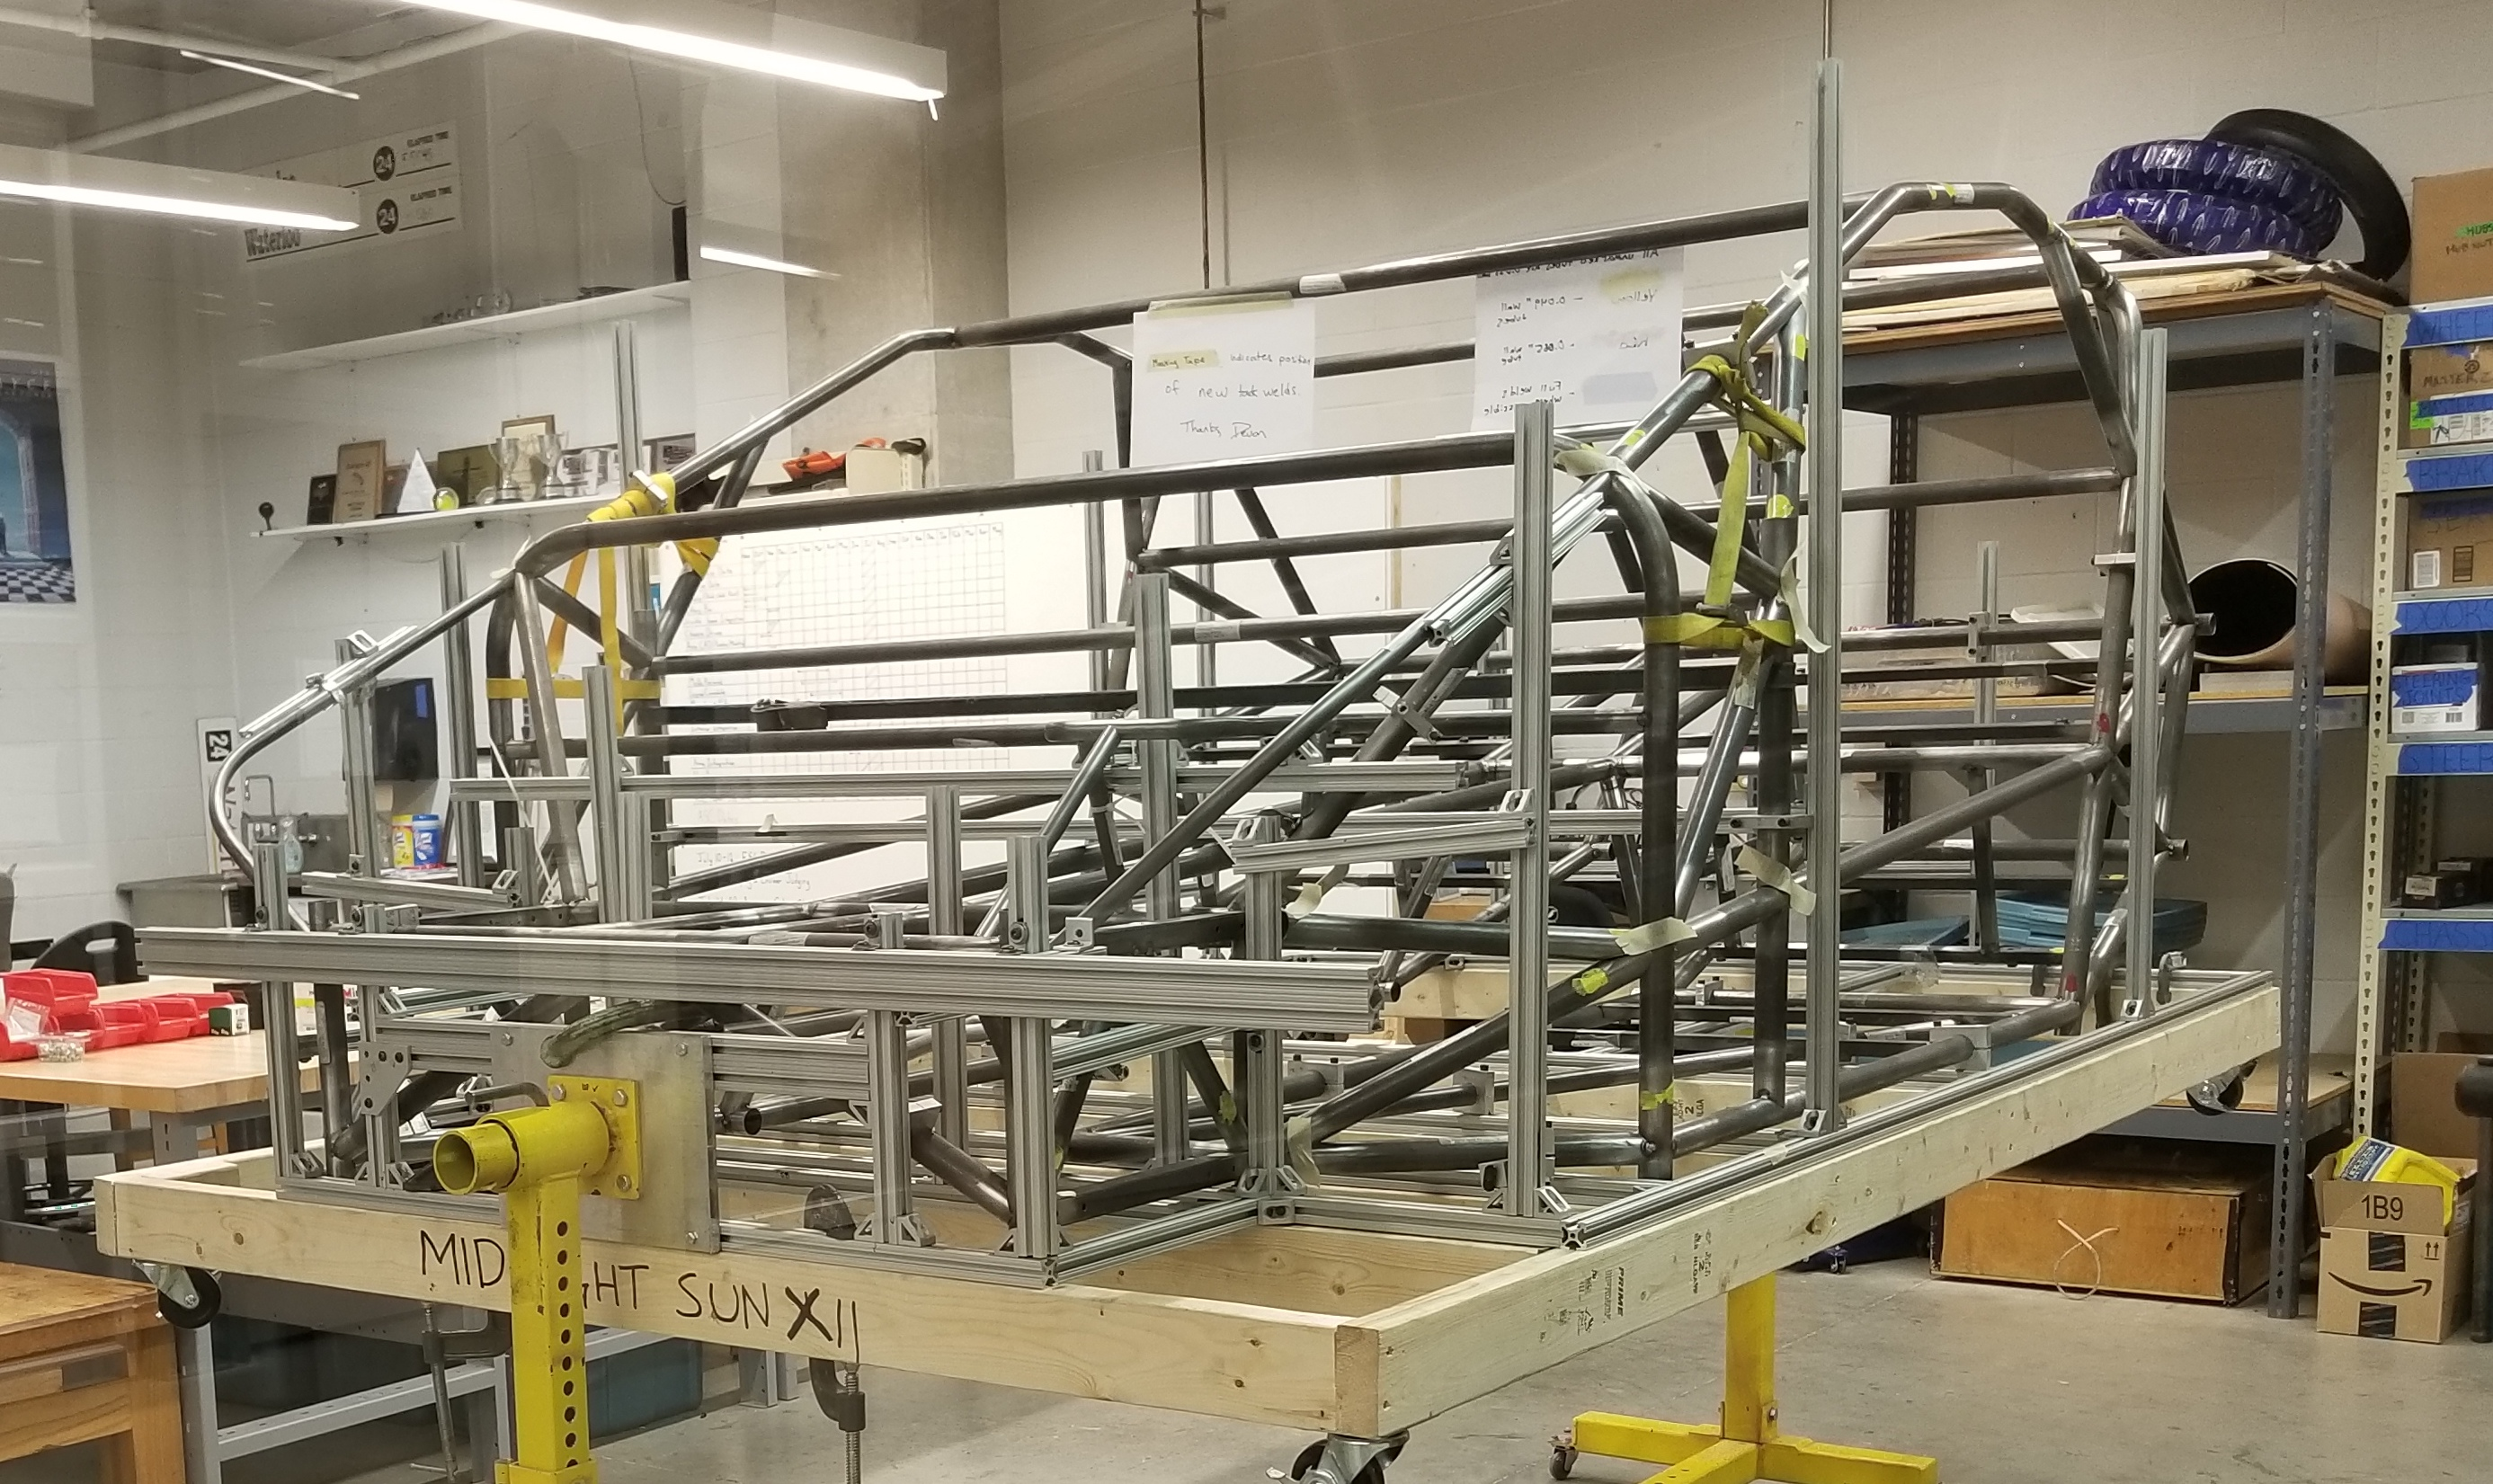
\includegraphics[width=0.75\textwidth]{figures/welding-jig}
\caption{Welding jig on rotating mount}
\label{fig:welding-jig}
\end{figure}

\subsection{Roll cage}
The roll cage is integrated into the design of the chassis members enclosing the occupant cell. For the purposes of ASC regulations, the roll cage can be considered to include the A and B pillar hoops and elements connecting these two hoops lengthwise through the car. For clarity, these elements have been highlighted in Figure \ref{fig:roll-cage}.

\begin{figure}
\centering
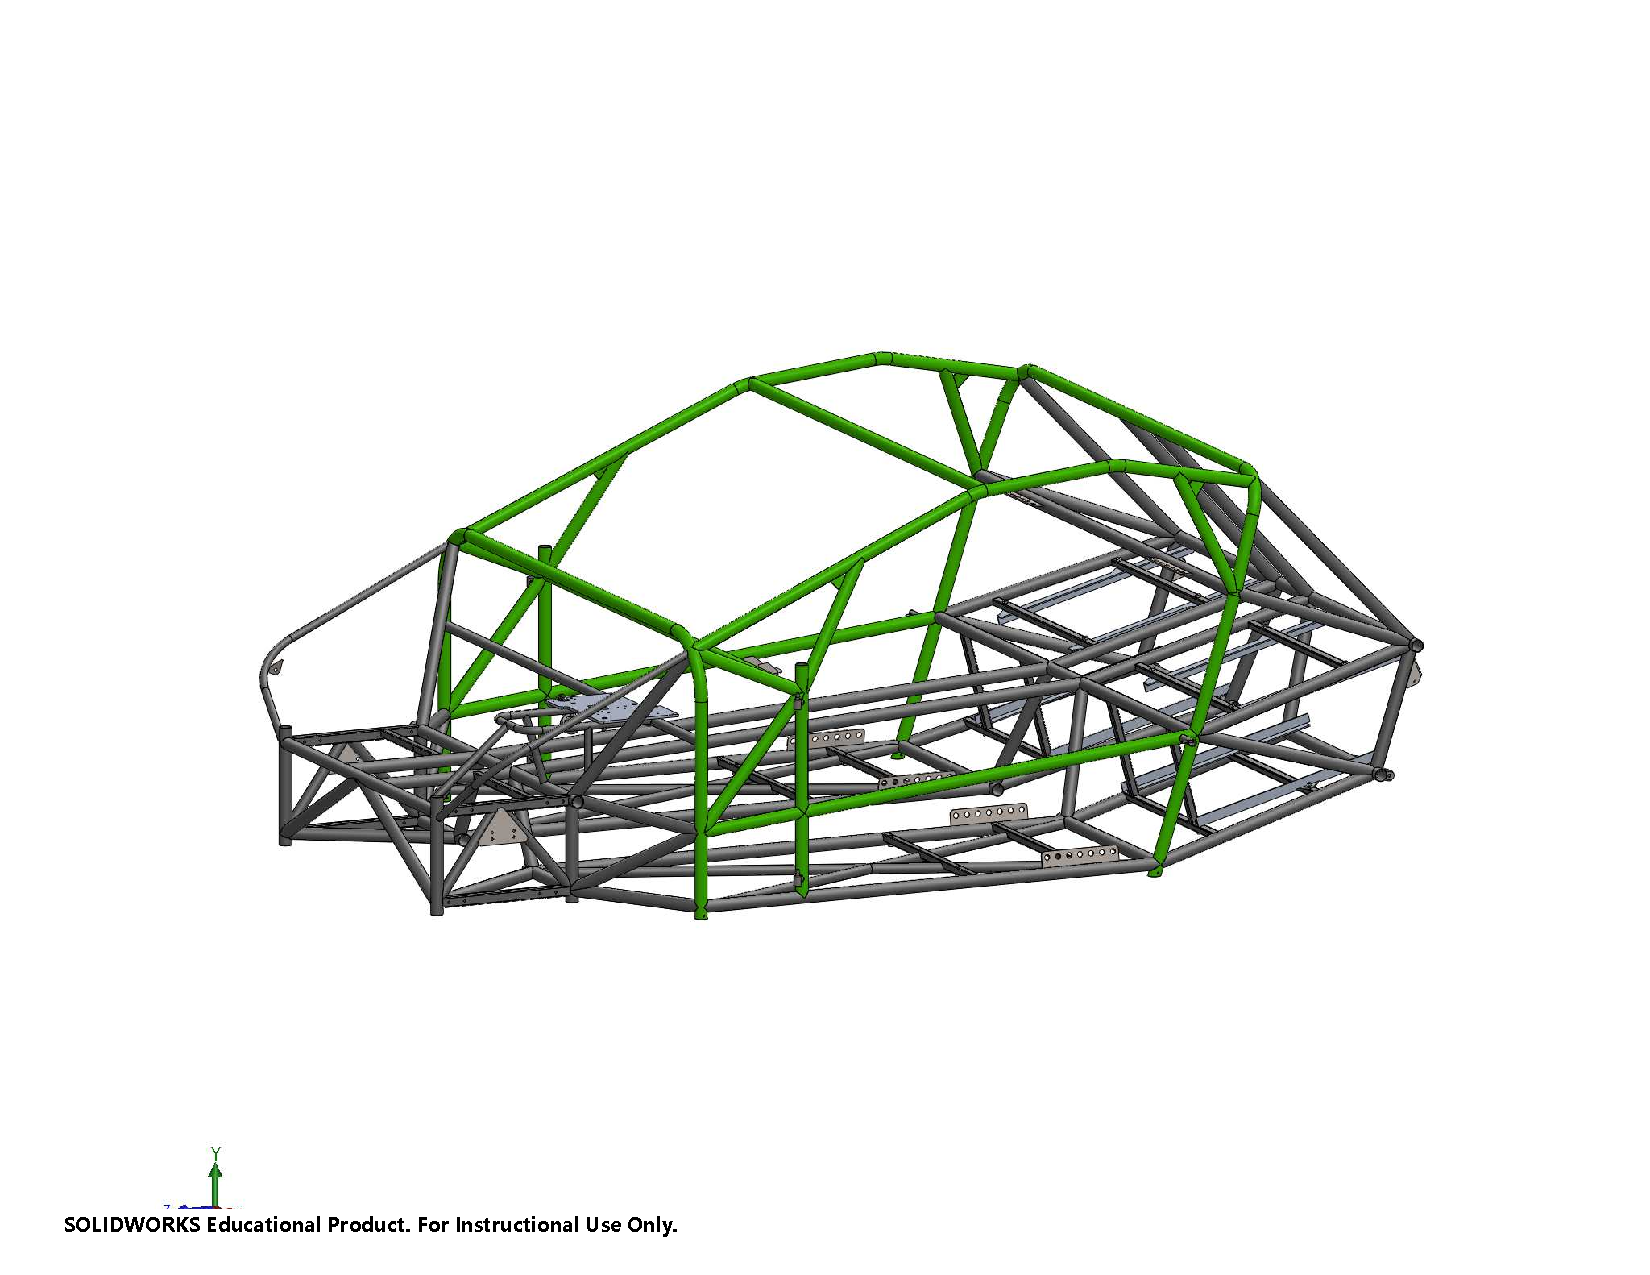
\includegraphics[width=0.75\textwidth]{figures/roll-cage}
\caption{Chassis with roll cage elements highlighted}
\label{fig:roll-cage}
\end{figure}


\section{Seat belts}
MSXII is equipped with 5-point seat belts for both occupants. Seat belt hardpoints are mounted to metal tabs welded to chassis members, shown in Figure \ref{fig:seat-belt-tab-positions}. Figure \ref{fig:seat-belt-tab} shows one of these tabs. Figures \ref{fig:seat-belt-side-view} and \ref{fig:seat-belt-top-view} demonstrate compliance with ASC regulations 10.3.E.

\begin{figure}
\centering
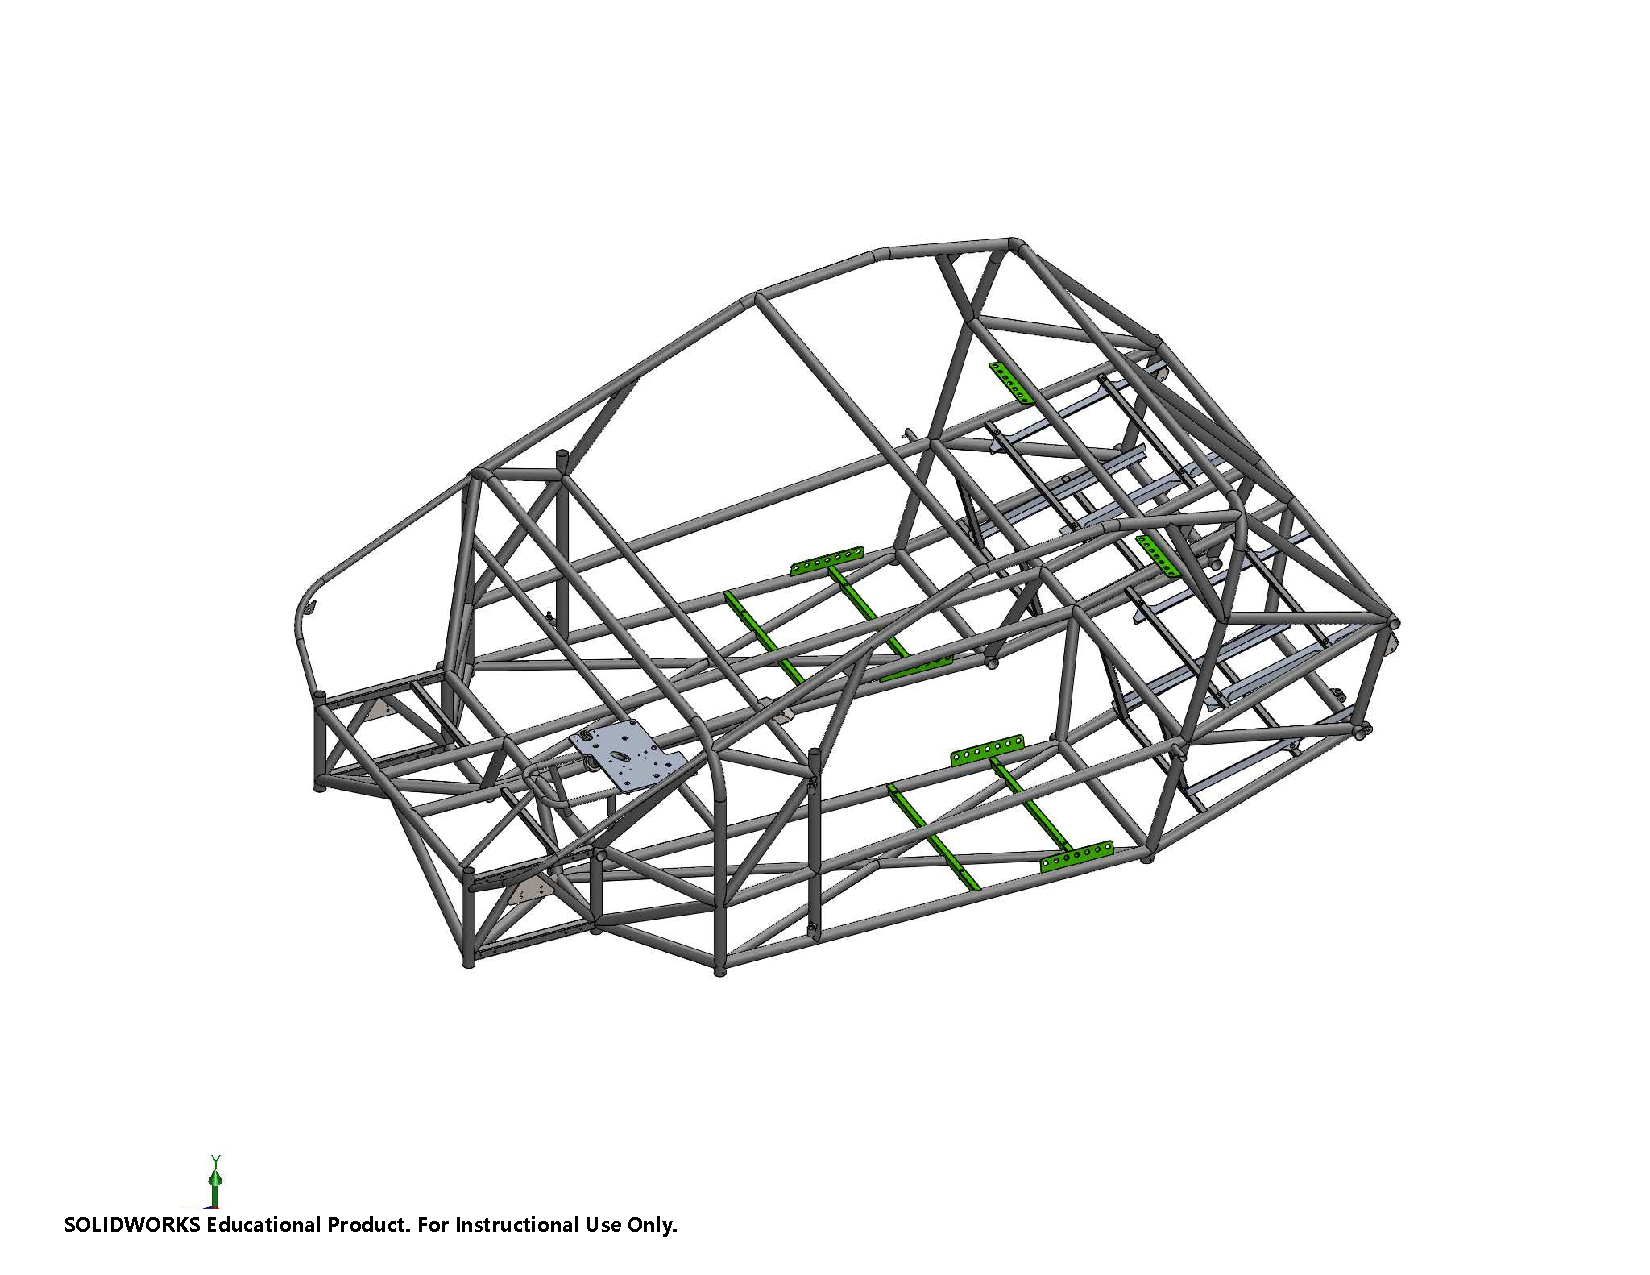
\includegraphics[width=0.75\textwidth]{figures/seat-belt-tab-positions}
\caption{Chassis mounting points for seat belts}
\label{fig:seat-belt-tab-positions}
\end{figure}

\begin{figure}
\centering
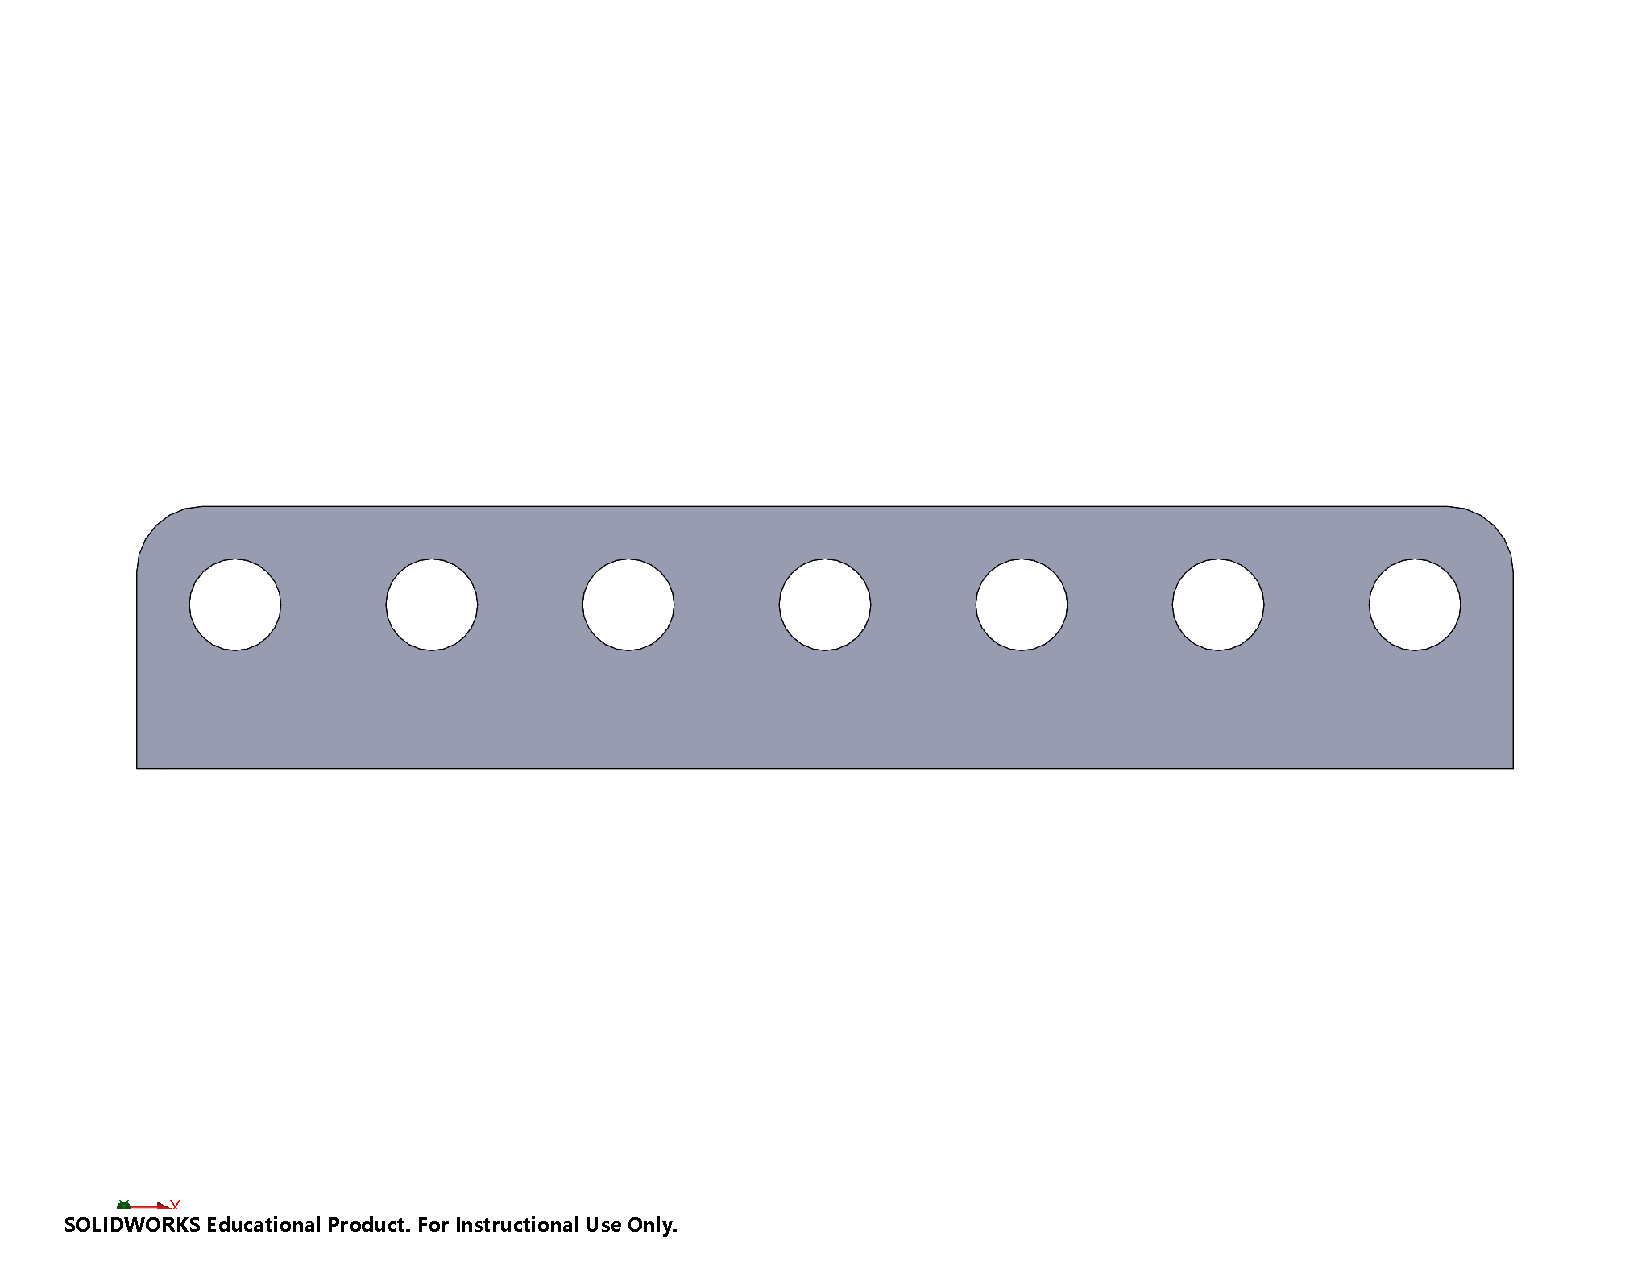
\includegraphics[width=0.75\textwidth]{figures/seat-belt-tab}
\caption{Single seat belt tab}
\label{fig:seat-belt-tab}
\end{figure}

\begin{figure}
\centering
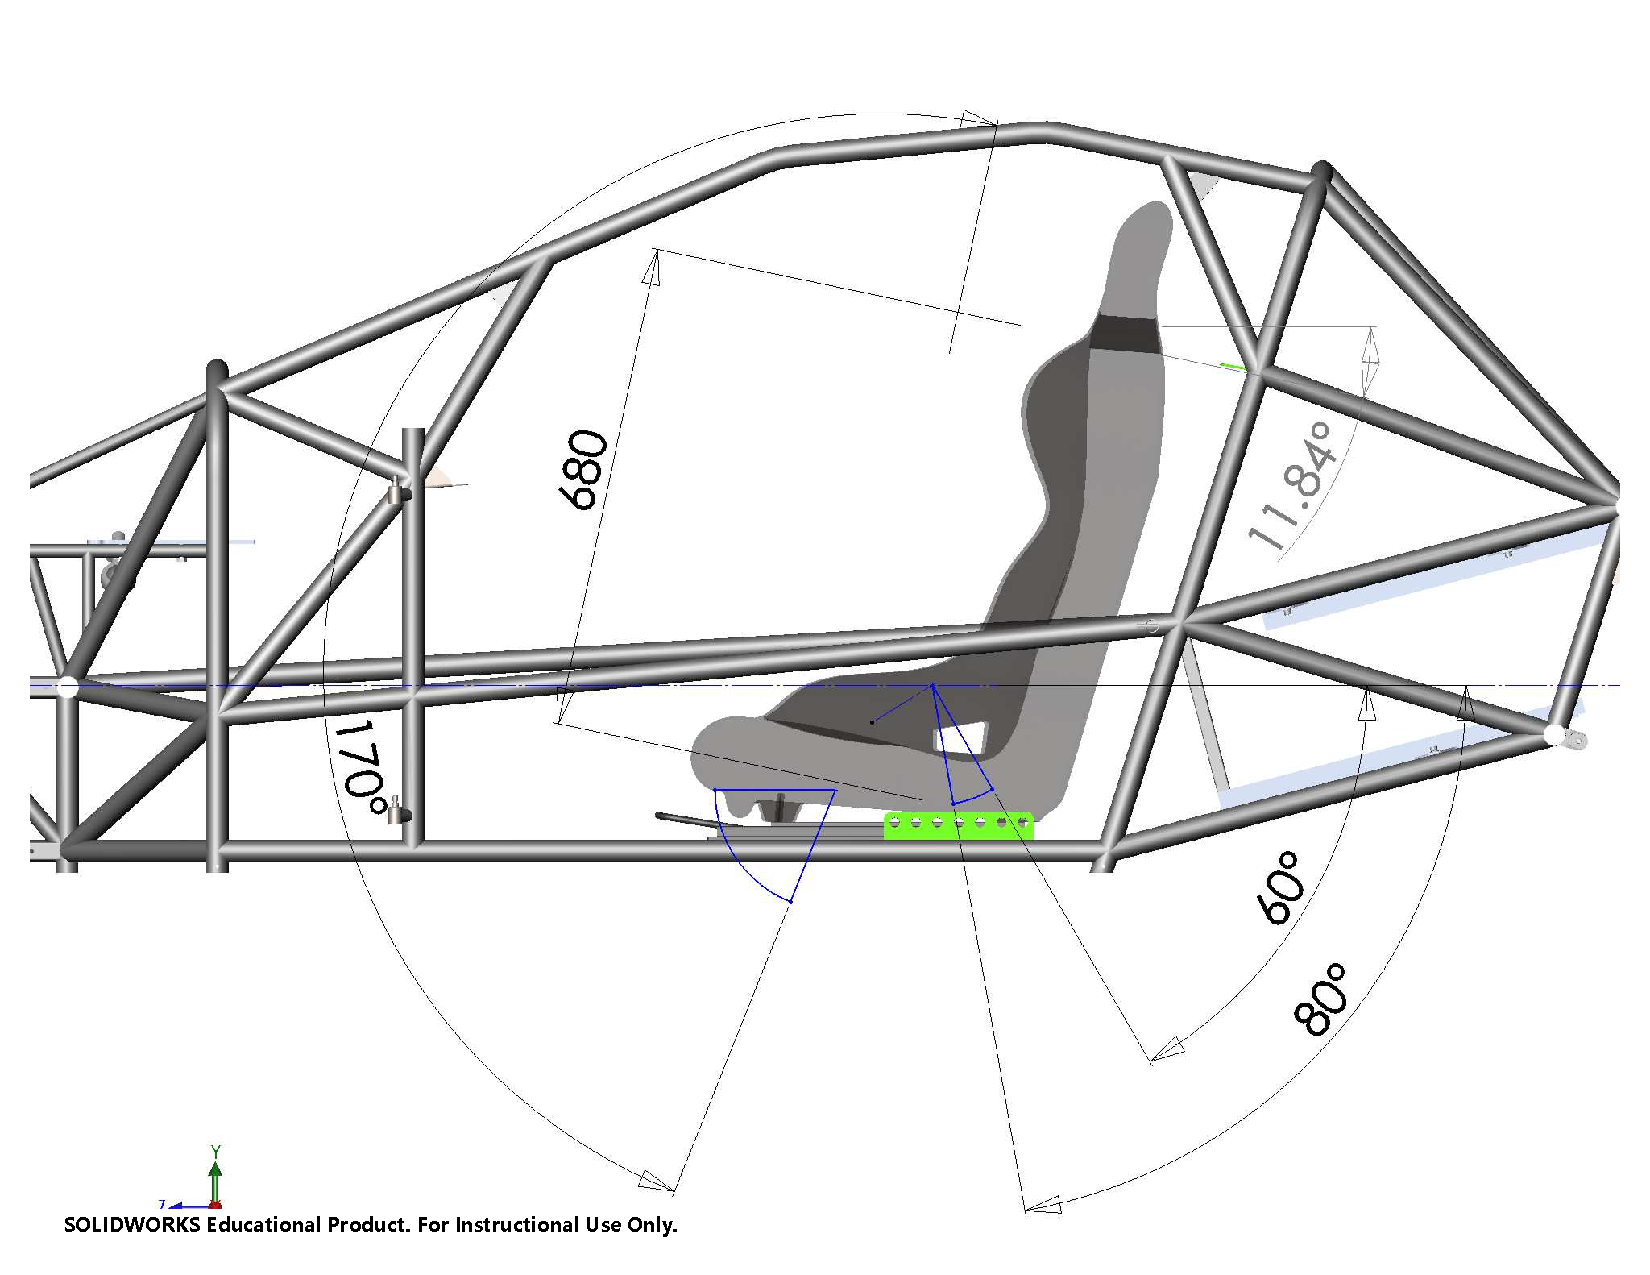
\includegraphics[width=0.75\textwidth]{figures/seat-belt-side-view}
\caption{Side view of seat belt geometry}
\label{fig:seat-belt-side-view}
\end{figure}

\begin{figure}
\centering
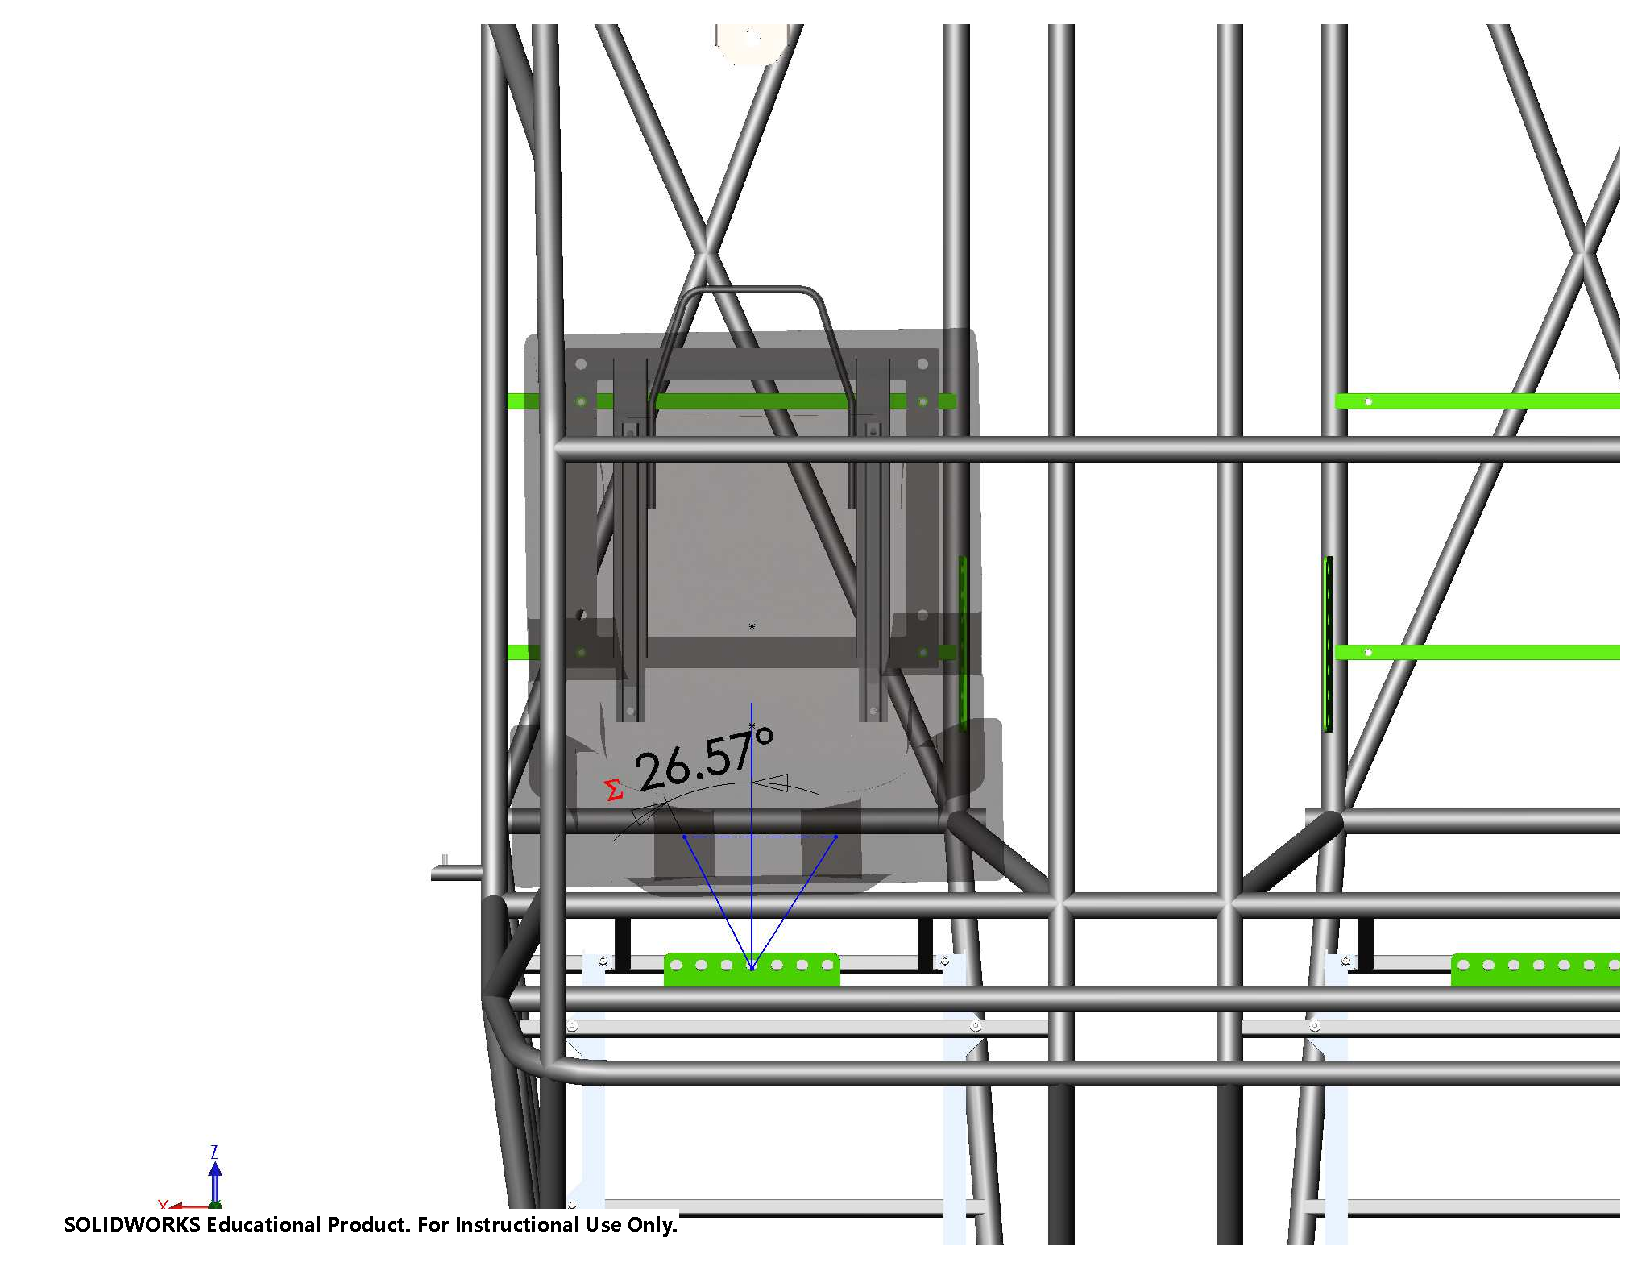
\includegraphics[width=0.75\textwidth]{figures/seat-belt-top-view}
\caption{Top view of seat belt geometry}
\label{fig:seat-belt-top-view}
\end{figure}

\section{Braking system}
\subsection{Primary brakes}
The primary braking system is designed with dual redundant front braking, consisting of two identical systems with separate master cylinders, hydraulic lines, and calipers to each of the left and right wheels. The master cylinders are operated in unision via a single mechanical brake pedal. A schematic of the primary system is shown in Figure \ref{fig:primary-brakes-schematic}.

\begin{figure}
\centering
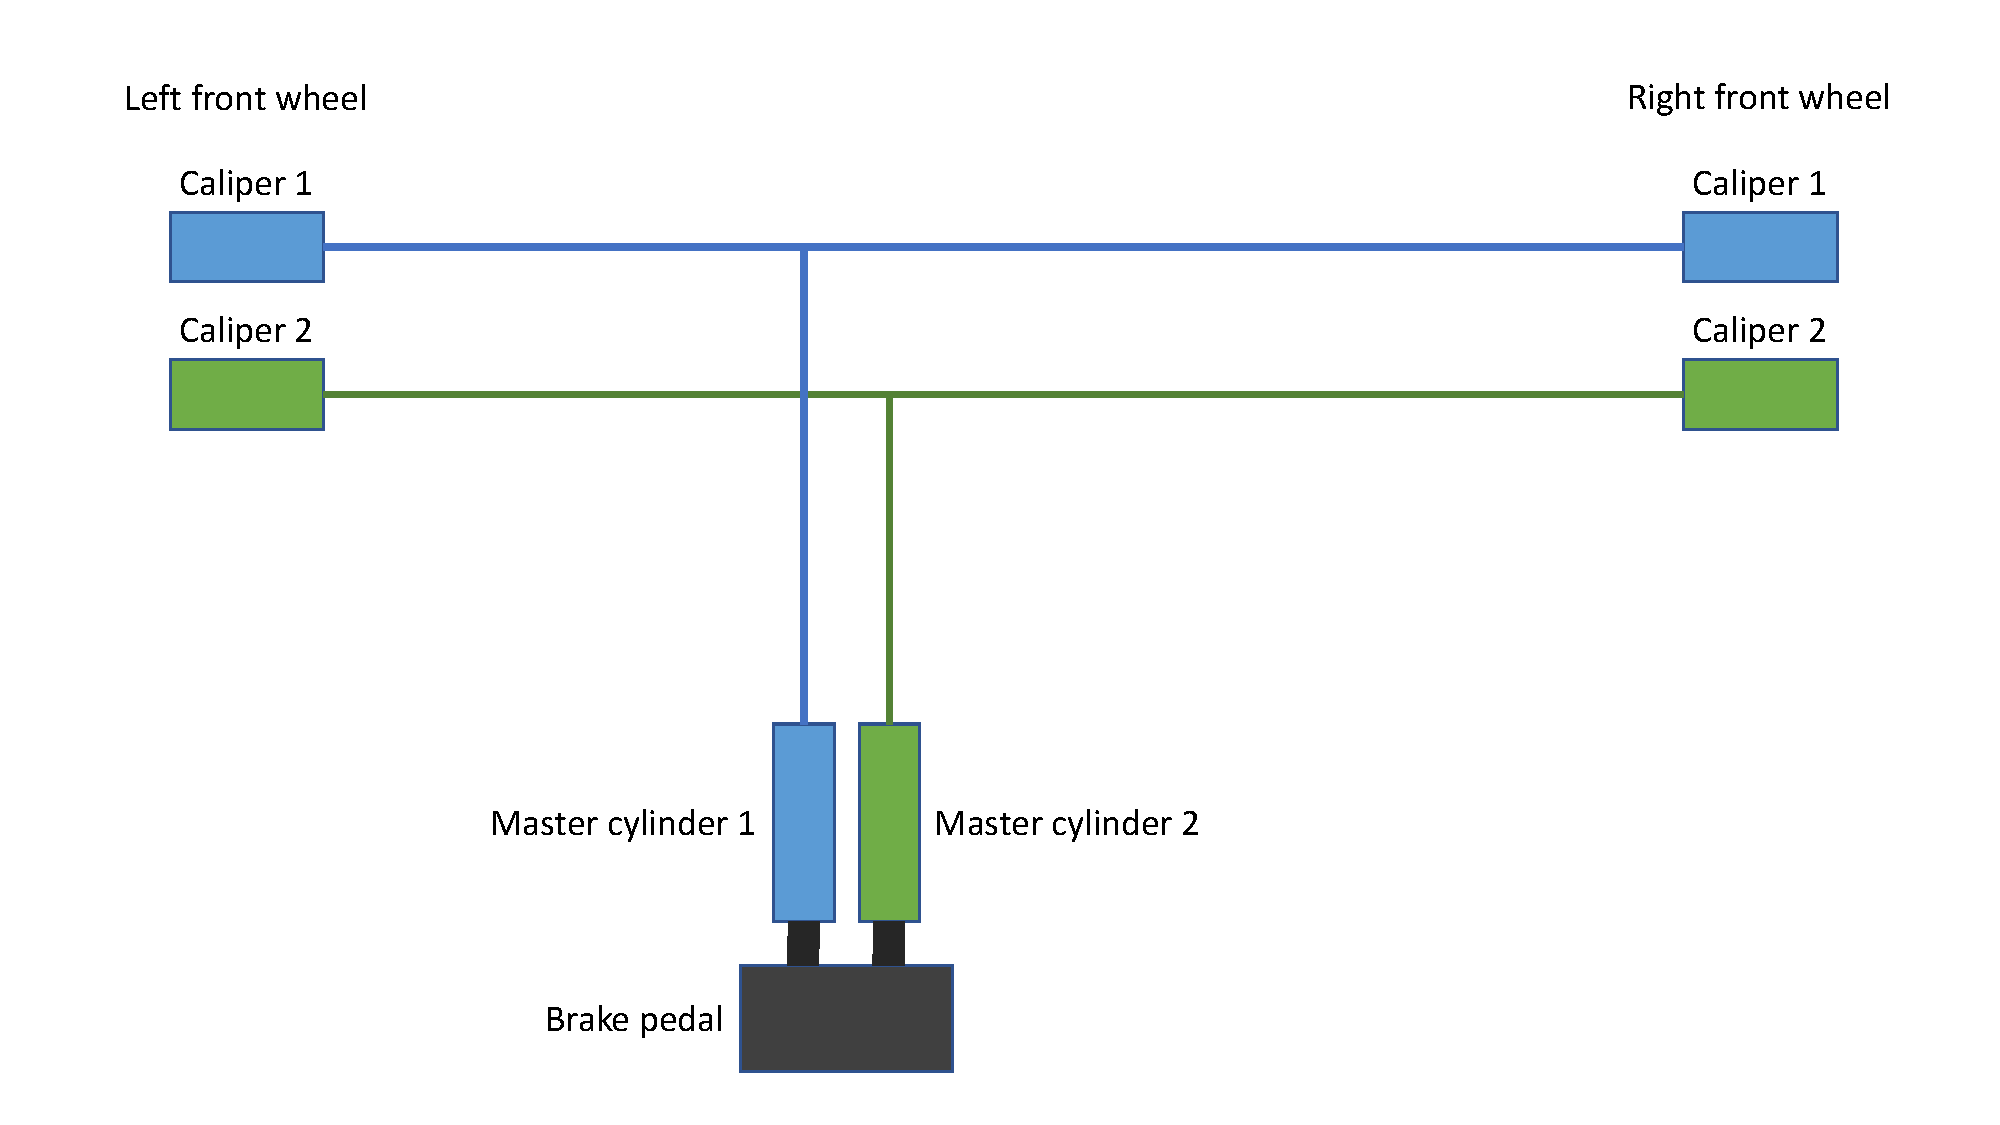
\includegraphics[width=\textwidth]{figures/primary-brakes-schematic}
\caption{Schematic of primary braking system}
\label{fig:primary-brakes-schematic}
\end{figure}

Front brake calipers are Willwood parts \href{http://www.wilwood.com/Calipers/CaliperProd.aspx?itemno=120-8374}{120-8374} (left) and \href{http://www.wilwood.com/Calipers/CaliperProd.aspx?itemno=120-8373}{120-8373} (right). Willwood's website indicates the caliper pads have \SI{2}{in\squared} (\SI{12.9}{\centi\metre\squared}) contact area and 0.30" (\SI{7.6}{\milli\metre}) depth including the backing plate.

The master cylinders are Willwood part \href{http://www.wilwood.com/MasterCylinders/MasterCylinderProd.aspx?itemno=260-3374}{206-3374}. They have a 3/8"-24 outlet size which will need to be connected via a suitable brake line to the M10 x 1.25 inlets of the calipers. Brake lines will be DOT-approved hose assemblies sized for 3/8"-24 on one end and M10 on the other end via a banjo joint. The brake pedal is Willwood part \href{http://www.wilwood.com/Pedals/PedalProd.aspx?itemno=340-15079}{340-15079} and is mounted in the standard configuration to the left of the accelerator pedal.

Brake rotors will be custom-machined to the disk thickness and diameter supported by the Willwood calipers. All mounting geometry on the suspension upright for primary calipers are designed to position the primary calipers in the optimal positions to meet braking specifications.

\subsection{Parking brake}
The parking brake will be implemented by a cable-actuated caliper mounted at one of the front wheels. The caliper is the Tolomatic ME10LA, part number \href{https://www.tolomatic.com/products/product-details/me10-mechanical-disc-brake#/specs-order}{0732-0003}. It will share the same brake disk as the primary braking system but is otherwise mechanically independent. Due to unresolvable dimensioning differences between the Tolomatic and Willwood calipers, the parking brake caliper cannot be mounted perfectly as per the manufacturer's recommendations and will have only 80\% overlap with the brake disk. However, this is expected to provide more than sufficient countertorque to keep the vehicle stationary as per ASC regulations 10.6.

Figure \ref{fig:calipers-mounting-geometry} shows a front suspension upright with all three calipers mounted (two primary and one parking).

\begin{figure}
\centering
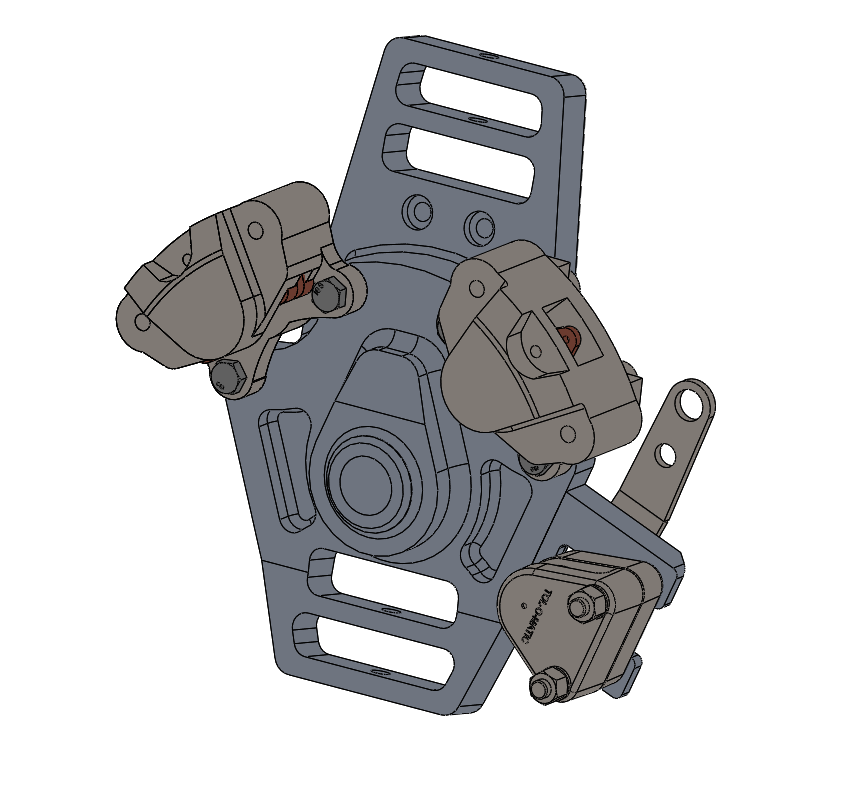
\includegraphics[width=0.5\textwidth]{figures/caliper-mounting-geometry}
\caption{View of dual-primary calipers and parking caliper on front suspension upright }
\label{fig:calipers-mounting-geometry}
\end{figure}

\section{Steering system}
The steering system uses a rear-steering, left-hand-drive rack and pinion from Helix (part number \href{http://www.helixsuspension.com/catalog/Steering/Manual-Steering-Racks/HEXSR5/Omni-Manual-Steering-Rack---Rear-Steering}{188754}). The system uses a collapsible steering column from Sweet Mfg.\@, part number \href{https://sweetmfg.biz/product.php?productid=2836}{405-10310}. The linkage uses dual U-joints to circumvent interfering brake system components and is shown in Figure \ref{fig:steering-assembly}.

\begin{figure}
\centering
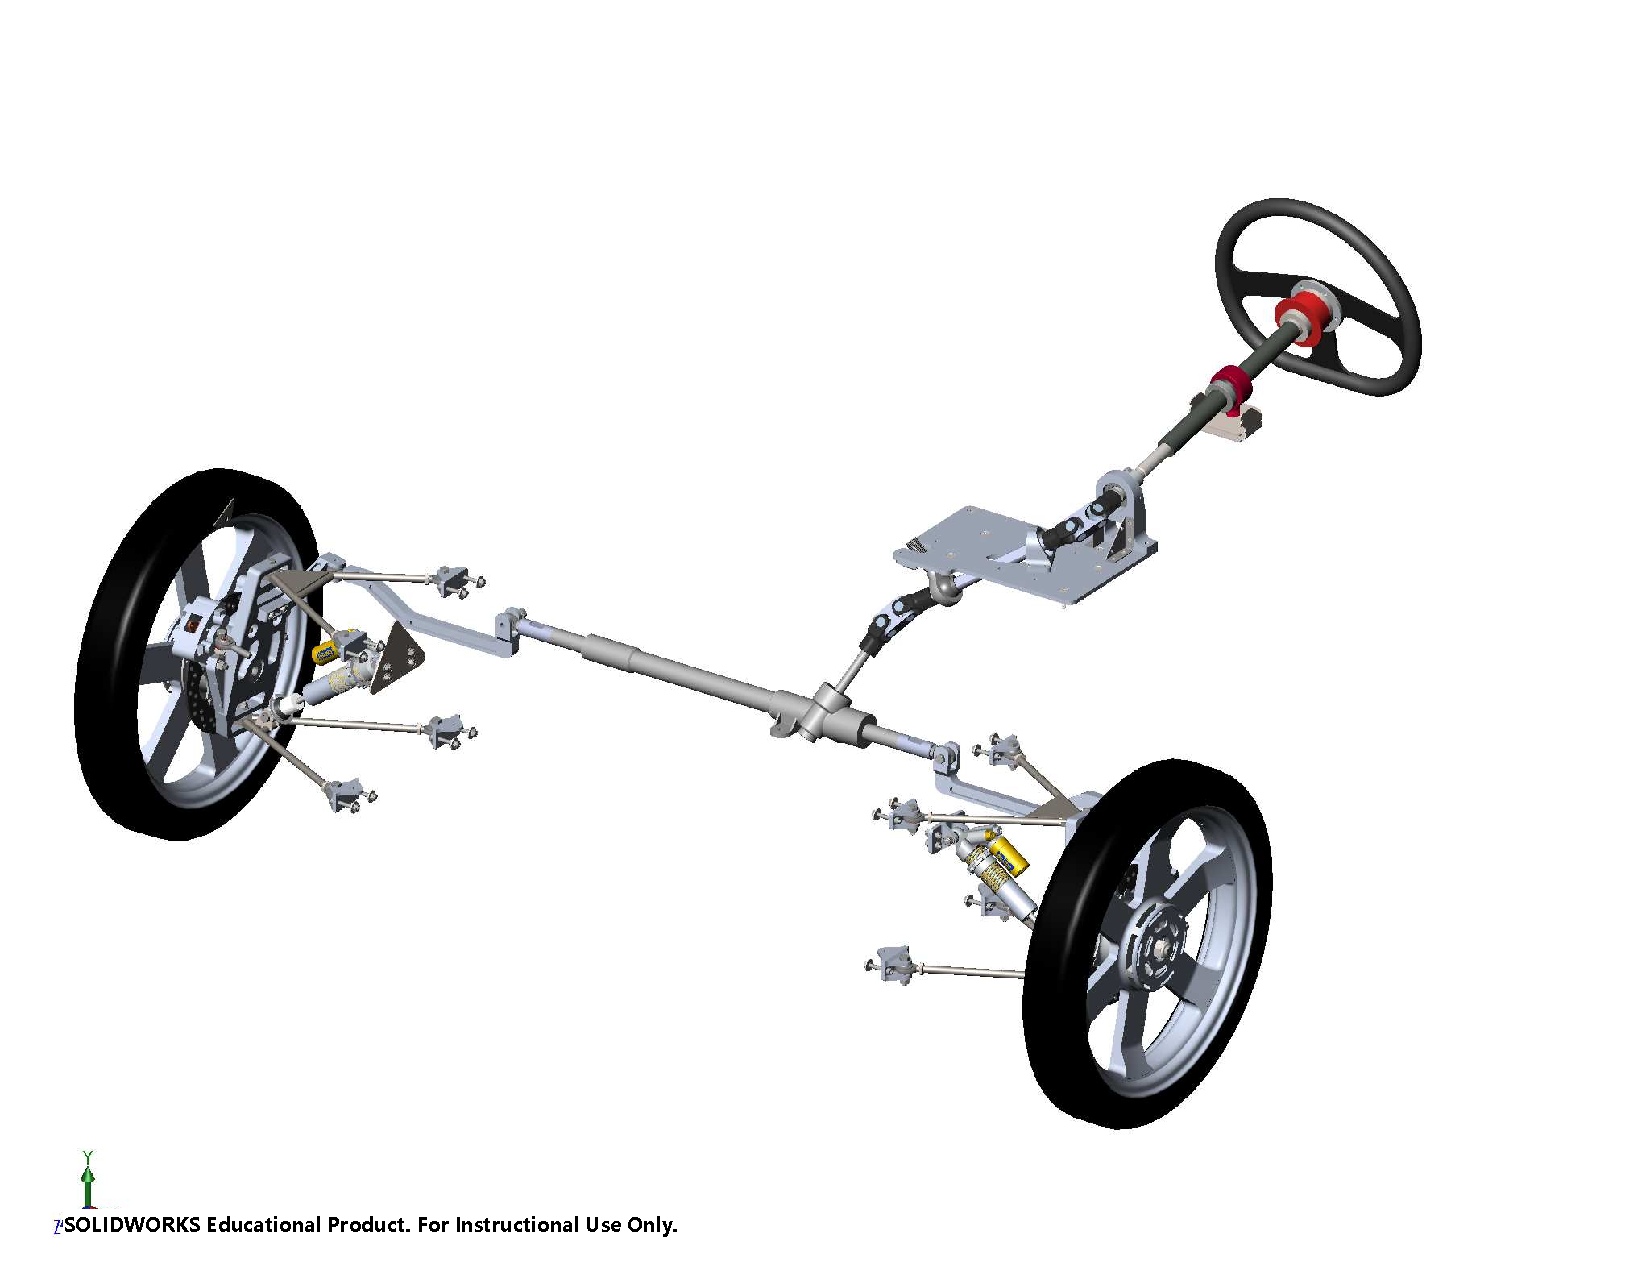
\includegraphics[width=0.75\textwidth]{figures/steering-assembly}
\caption{View of steering assembly}
\label{fig:steering-assembly}
\end{figure}

\section{Suspension}
\subsection{Front suspension}
The front suspension uses dual A-arms with an outboard dampener and coilover spring. The upper and lower control arms are custom-built from 4130 chromoly tubes. The dampener and coilover are a single integrated assembly supplied by \"Ohlins, sold as the TTX25, which is marketed for Formula SAE vehicles. Figure \ref{fig:front-suspension} shows the front suspension assembly.

\begin{figure}
\centering
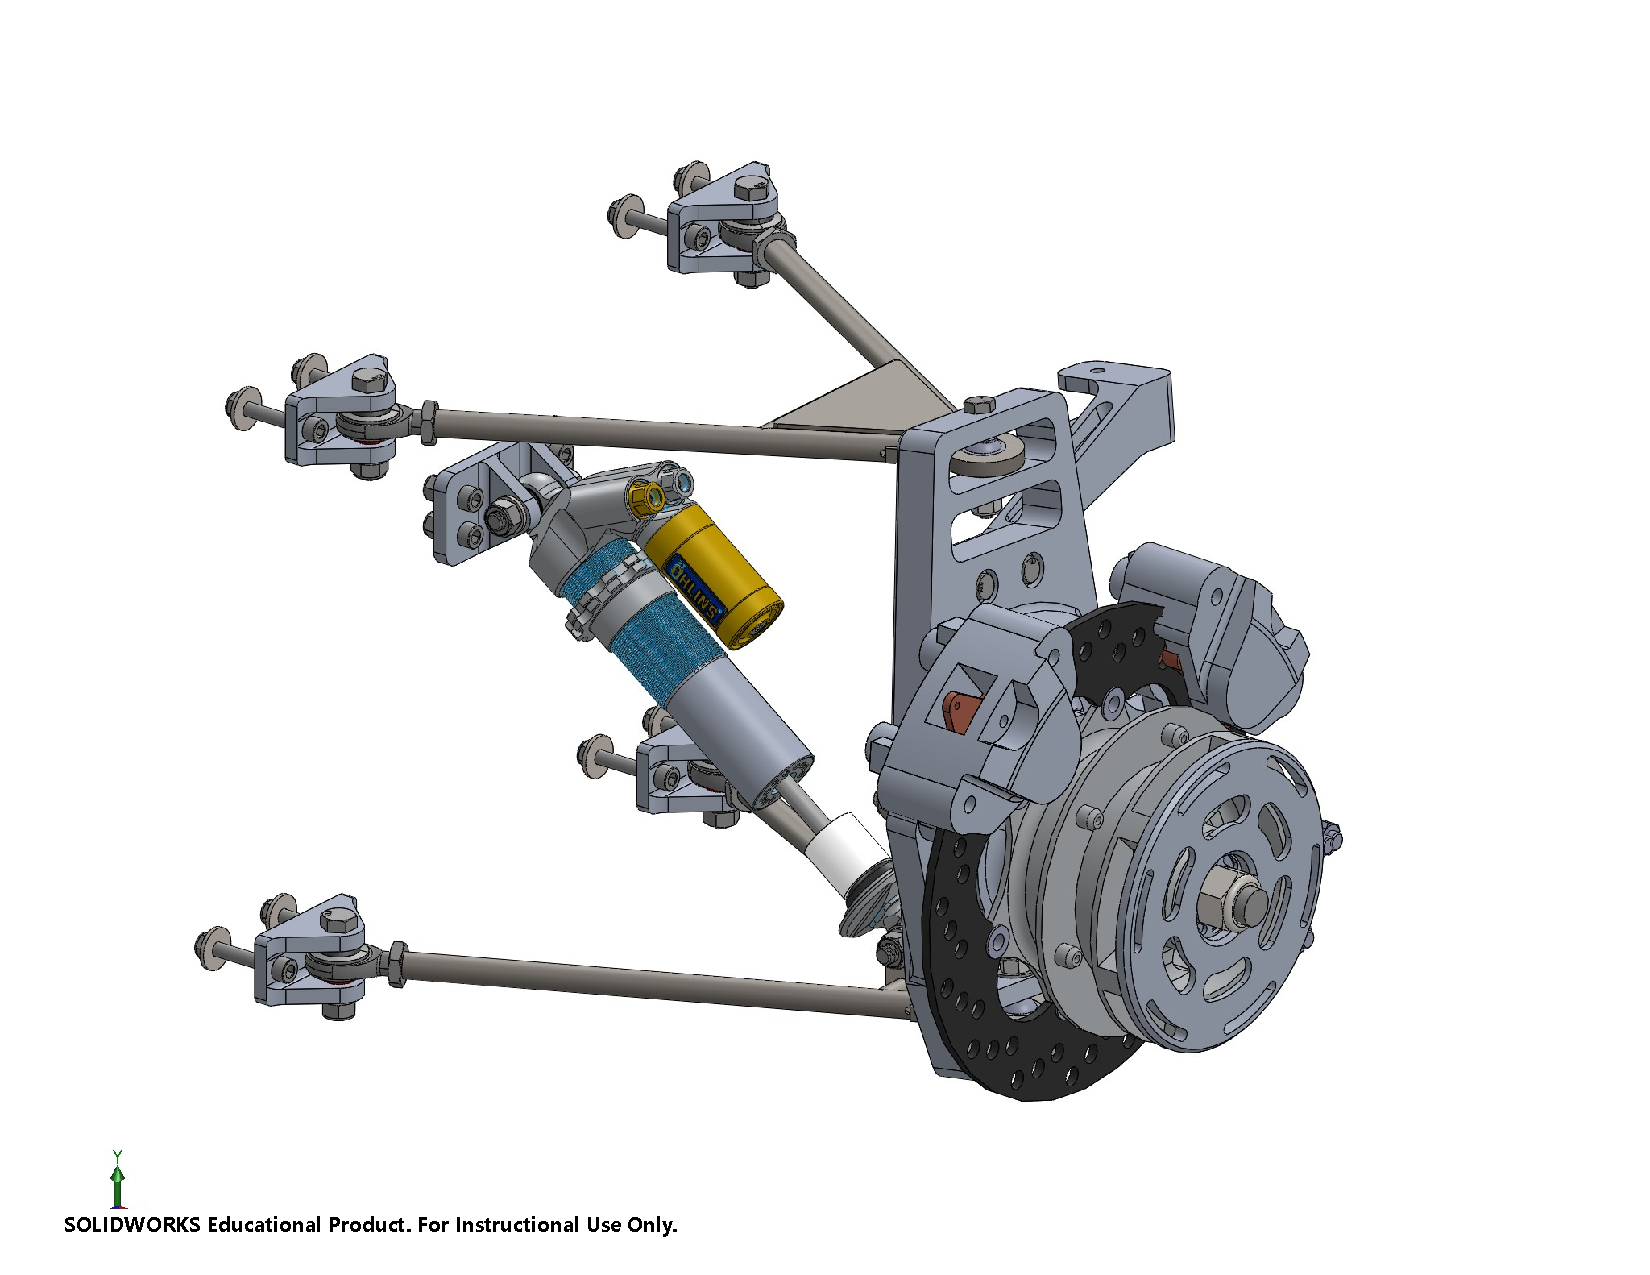
\includegraphics[width=0.75\textwidth]{figures/front-suspension}
\caption{View of front suspension assembly (parking brake caliper obstructed by hub)}
\label{fig:front-suspension}
\end{figure}

The front suspension lower control arm bears the majority of the shear stress from road forces. Based on hand calculations for a cantilever beam, the worst-case von Mises stress is \SI{183}{\mega\pascal}. This dictates the sizing of the rod end.

\subsection{Rear suspension}
The rear suspension uses independent trailing arms mounted outwards from the rear of the chasssis. The trailing arm itself is custom-machined and mounts the same \"Ohlins TTX25 shock absorber as the front suspension. Figure \ref{fig:rear-suspension} shows the rear suspension assembly.

\begin{figure}
\centering
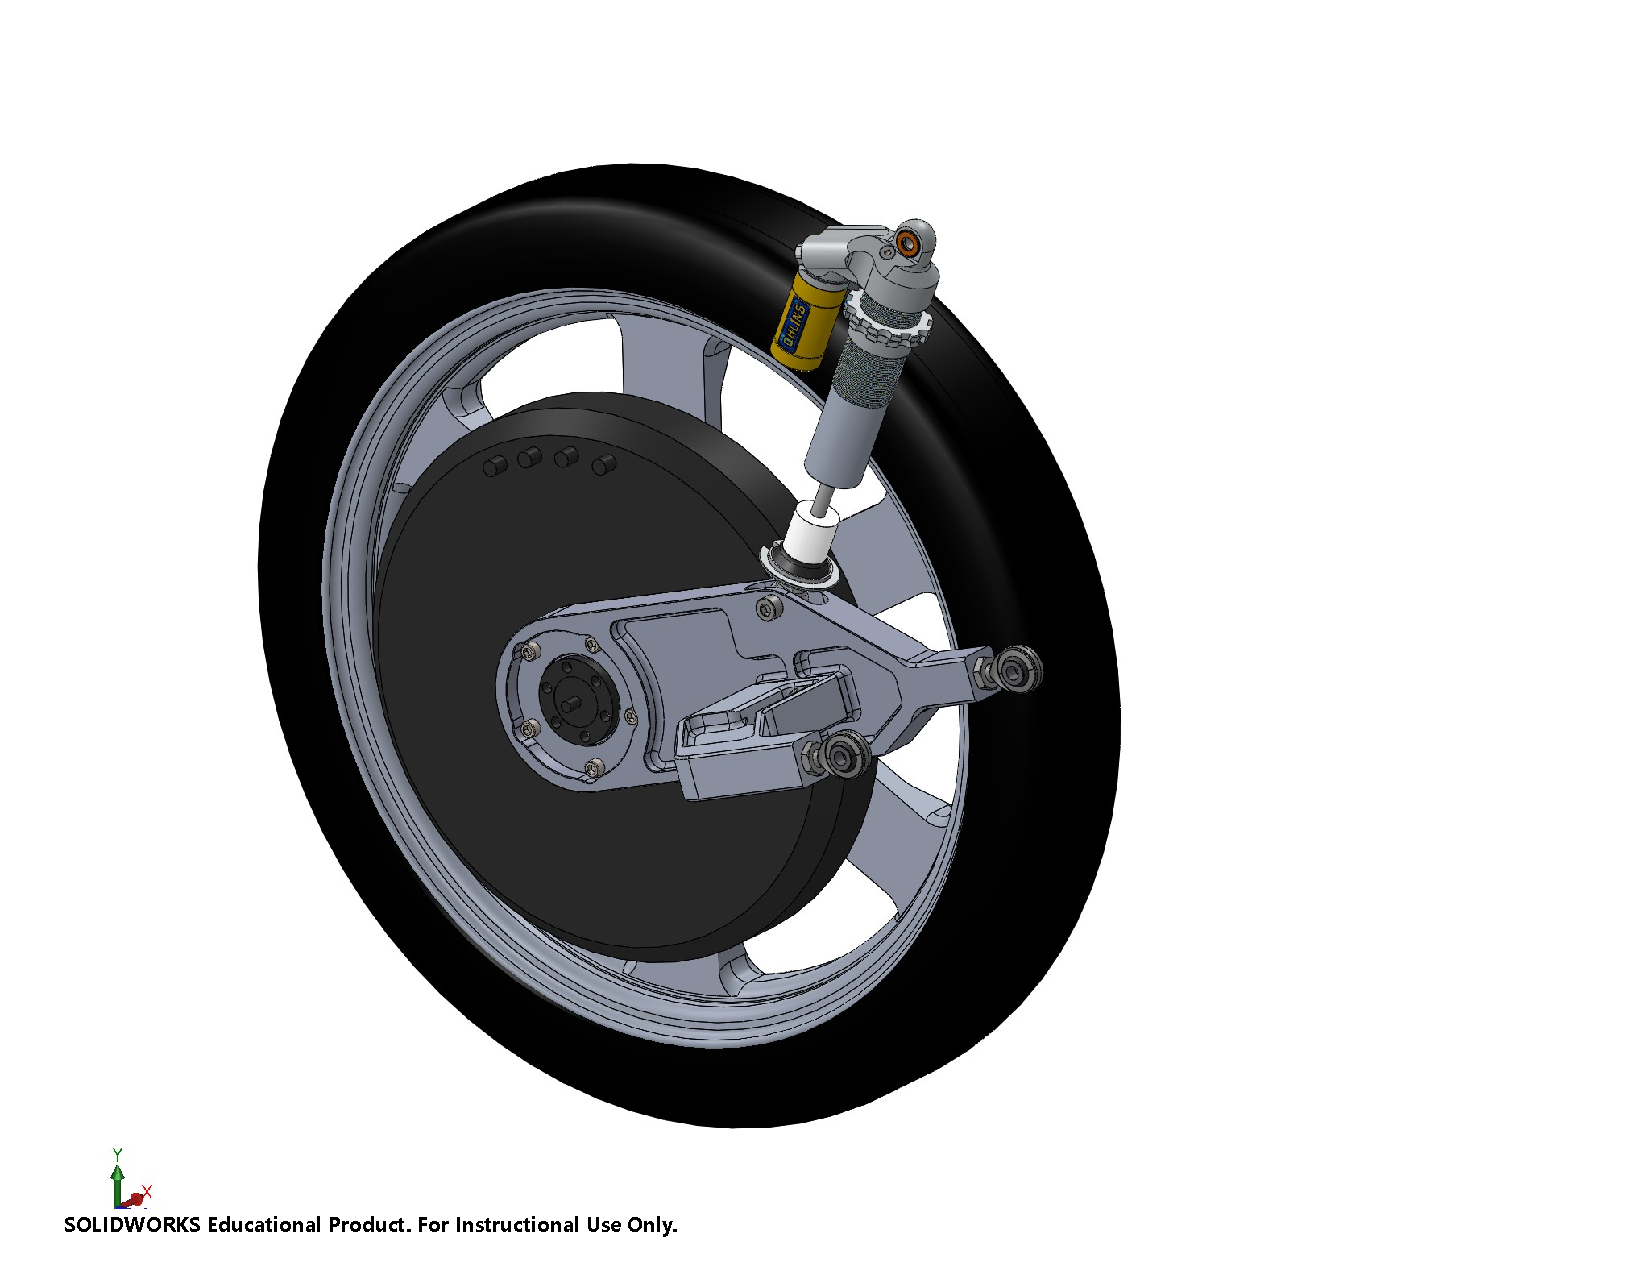
\includegraphics[width=0.75\textwidth]{figures/rear-suspension}
\caption{View of rear suspension assembly}
\label{fig:rear-suspension}
\end{figure}

\section{Finite element analysis}
Finite element analysis was performed using ANSYS on the chassis and all suspension and steering components (downstream from the rack and pinion). FEA of the chassis followed the specifications provided by the ASC regulations. A general methodology was to fix a solid beam or wall in space, and apply a 5G acceleration to the chassis against it. Images for FEA simulations of each requested scenario are shown in Appendix \ref{sec:fea-chassis-images}.

Worst-case loading forces on each wheel were used to derive appropriate contraints and forces for FEA simulation of the suspension and steering system. A complete derivation and summary of loading forces on each wheel is given in Appendix \ref{sec:loading-conditions}. Images of all FEA simulations for suspension and steering are available in Appendix \ref{sec:fea-parts-images}.

\subsection{Front suspension}
\subsubsection{Clevises}
Hand calculations were used to resolve the forces from the road as loading onto the clevises. The back face of the clevis was constrained with compresion only support. Cylindrical supports were used for the bolt holes and fastener pretension was added. Frictional contacts were added between the fasterners and the clevis.

\subsubsection{Upper control arms}
Contacts were modeled between the control arm tubes and the bearing plate. Forces were applied to the bearing plate based on hand calculations.

\subsubsection{Lower control arms}
Contacts were modeled between the control arm tubes and the mounting tabs on the coilover clevis. Forces were applied to the profile that the bearing sits in, based off of hand calculations.

\subsubsection{Uprights}
A dummy wheel was modeled to which forces were applied. The dummy wheel contacted the spindle with a frictional contact which then applied a load to the upright. The brake forces were appled to the caliper mounting holes, assuming only one caliper was providing all braking force.

\subsubsection{Spindles}
A dummy wheel was modeled to which forces were applied. The dummy wheel contacted the spindle with a frictional contact which then applied a load to the upright.

\subsubsection{Upper bearing plates}
Contacts were modeled between the control arm tubes and the bearing plate. Forces were applied to the bearing plate based on hand calculations.

\subsubsection{Coilover control arm tabs}
The maximum force on the front wheel was resolved as a compressive load in the coilover and applied to this tab.

\subsubsection{Coilover mounting plates}
Hand calculations were used to resolve the forces from the road as loading onto the clevises. For this simulation a frictional contact was added between the clevis and the mounting plate. Dummy chassis tubes were modeled behind the mounting plate and welded edges were fixed.

\subsection{Rear suspension}
\subsubsection{Clevises}
The worst case of four loading scenarios was taken (2 clevis positions, each with either the inside or outside wheel when rounding a corner). It was assumed that all lateral force was applied to a single clevis because otherwise this is a statically indeterminate problem on paper.

\subsubsection{Coilover tabs}
The maximum normal force and acceleration force on the rear wheel was resolved as a compressive load in the coilover and applied to this tab.

\subsubsection{Trailing arms}
Similar to the front suspension, the trailiing arm was simulated using a dummy wheel model. A force was applied to the contact patch and supports were added to the rod end, plain bearing and coilover clevis on the trailing arm.

\subsection{Steering}
\subsubsection{Steering arms}
A compression support was added on the face datuming off of the upright. The maximum lateral force on the tire during 1G cornering was resolved as a torque on the upright. This torque was applied by a bearing load acting at the end of the steering arm.

\subsubsection{Tie rods}
A similar analysis to that for the steering arm was used. Force was applied to one end of the tie rod while the other remained fixed. Both sides of the tie rod were tested with an applied force and fixed support.

\subsection{Results}
All FEA results for suspension and steering components are summarized in Table \ref{tab:fea-results-suspension-steering}.

\begin{table}
\centering
\begin{tabular}{lllrr}
\toprule
Part Number & Part Name                    & Material             & Max Stress (\si{\mega\pascal}) & Safety Factor \\
\midrule
MS00015     & Coilover Clevis              & Aluminum, 7075       &                 147 &           3.4 \\
MS00029     & Upper Control Arm Clevis     & Aluminum, 7075       &                 191 &           2.6 \\
MS00102     & Lower Control Arm Clevis     & Aluminum, 7075       &                 198 &           2.5 \\
MS00017     & Upper Control Arm            & Chromoly Steel, 4130 &                 199 &           2.3 \\
MS00018     & Lower Control Arm            & Chromoly Steel, 4130 &                 226 &           2.0 \\
MS00019     & Upright                      & Aluminum, 7075       &                 210 &           2.4 \\
MS00020     & Spindle                      & Chromoly Steel, 4140 &                 177 &           2.3 \\
MS00030     & Upper Bearing Plate          & Chromoly Steel, 4130 &                 141 &           3.3 \\
MS00036     & Coilover Control Arm Tab     & Chromoly Steel, 4130 &                 159 &           2.9 \\
MS00038     & Coilover Mounting Plate      & Chromoly Steel, 4130 &                 147 &           3.1 \\
MS00086     & Rear Suspension Clevis Mount & Chromoly Steel, 4130 &                 231 &           2.0 \\
MS00047     & Rear Suspension Coilover Tab & Chromoly Steel, 4130 &                 147 &           3.1 \\
MS00065     & Trailing Arm                 & Aluminum, 7075       &                 263 &           1.9 \\
MS00074     & Steering Arm                 & Aluminum, 6061-T6    &                  77 &           3.5 \\
MS00101     & Tie Rod                      & Aluminum, 6061-T6    &                  41 &           6.6 \\
\bottomrule
\end{tabular}
\caption{Summary of FEA results for suspension and steering components}
\label{tab:fea-results-suspension-steering}
\end{table}

% Bibliography
%\pagebreak
%\printbibliography

% Appendix
\clearpage
\appendix
\section{Loading conditions}
\label{sec:loading-conditions}
FEA of the chassis, suspension, and steering system was done using ANSYS software. Loading conditions were derived from both ASC requirements and real-world scenarios. Assuming a smooth driving surface, the largest normal force acting on the front tire will occur while braking in a turn. Similarly, the largest normal force acting on the rear tire will occur while accelerating in a turn. To approximate these loading condition, the a superposition of two static half car models is used; one for cornering and one for hard braking.

Table \ref{tab:loading-conditions-params} lists vehicle parameters that are relevant in determining the loading conditions in the suspension. The mass and moment of inertia were computed using CAD software. 

\begin{table}
\centering
\begin{tabular}{lrl}
\toprule
Mass ($M$)                                  &  550 & \si{\kilo\gram}              \\
Wheelbase                                   & 2.60 & \si{\metre}                  \\
Track                                       & 1.60 & \si{\metre}                  \\
Tire Diameter                               & 0.53 & \si{\metre}                  \\
Wheel Assembly Moment of Inertia ($J_w$)    & 0.25 & \si{\kilogram\metre\squared} \\
Distance from Front Wheel to CoG ($a$)      & 1.32 & \si{\metre}                  \\
Distance from Front Wheel to CoG ($b$)      & 1.28 & \si{\metre}                  \\
Distance from Road to CoG ($h$)             & 0.52 & \si{\metre}                  \\
Full Wheel Travel in Compression            &   45 & \si{\milli\metre}            \\
Front Coilover Angle from Vertical          &   40 & \si{\degree}                 \\
Rear Coilover Angle from Vertical           &   30 & \si{\degree}                 \\
\bottomrule
\end{tabular}
\caption{Important vehicle parameters}
\label{tab:loading-conditions-params}
\end{table}

\subsection{Braking}
Figure \ref{fig:braking-fbd} shows a free body diagram of a half car model undergoing braking. The required braking force can be approximated as follows: 
\begin{equation}
F_\mathrm{braking} = F_\mathrm{Nf} + F_\mathrm{Nr} = Mg = (\SI{550}{\kilo\gram})(\SI{9.81}{\metre\per\second\squared}) = \SI{5.40}{\kilo\newton}
\end{equation}
From Figure \ref{fig:braking-fbd}, summing the moments about the centre of gravity and the vertical forces results in the following equations: 
\begin{gather}
aF_\mathrm{Nf} = hF_\mathrm{braking} + bF_\mathrm{Nr} \\
F_\mathrm{Nf} + F_\mathrm{Nr} = Mg
\end{gather}
Solving for the front normal force: 
\begin{equation}
\begin{split}
aF_\mathrm{Nf} &= hF_\mathrm{braking} + b(Mg - F_\mathrm{Nf})\\
F_\mathrm{Nf} &= \frac{hF_\mathrm{braking} + bMg}{a+b} = \frac{(\SI{0.52}{\metre})(\SI{5.40}{\kilo\newton})+(\SI{1.28}{\metre})(\SI{550}{\kilo\gram})(\SI{9.81}{\metre\per\second\squared})}{(\SI{1.32}{\metre})+(\SI{1.28}{\metre})} = \SI{3.74}{\kilo\newton}
\end{split}
\end{equation}
Note that \SI{3.74}{\kilo\newton} is for both front wheels. Therefore there is approximately \SI{1.87}{\kilo\newton} of normal force on each front tire during hard braking. 

\begin{figure}
\centering
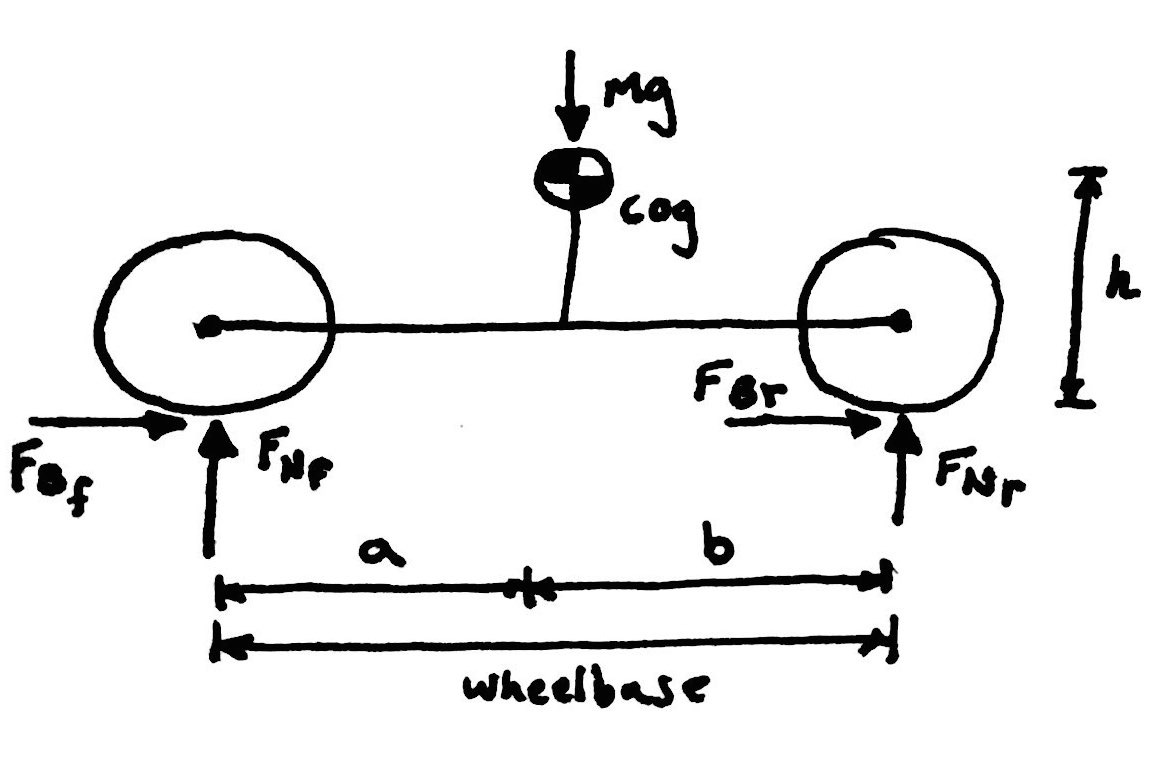
\includegraphics[width=.5\textwidth]{figures/braking-fbd}
\caption{Free body diagram of vehicle braking}
\label{fig:braking-fbd}
\end{figure}

\subsection{Acceleration}
MSXII uses NGM SCM-150 motors which have a peak torque of \SI{135}{\newton\metre}. From this torque value and a number of other vehicle parameters the vehicle's maximum acceleration can be calculated as follows: 
\begin{gather}
a = \frac{F_w}{\frac{1}{2}M} \\
\alpha_w = \frac{T_m - F_wr}{J_w} \\
\alpha_w = ar
\end{gather}
where $a$ is the acceleration of the vehicle, $F_w$ is the friction force acting on a single tire while accelerating, $J_w$ is the moment of inertia of the wheel assembly, $r$ is the radius of the tire, $T_m$ is the torque from the motor and $\alpha_w$ is the angular acceleration of the wheel. 

Rearranging the above three equations, the acceleration of the vehicle can be expressed as a function of motor torque as follows: 
\begin{equation}
\begin{split}
a &= \frac{T_m r}{\frac{1}{2}Mr^2 + J_w} \\
a &= \frac{(\SI{135}{\newton\metre})(\SI{0.27}{\metre})}{\frac{1}{2}(\SI{550}{\kilo\gram})(\SI{0.27}{\metre\squared})^2 + \SI{0.25}{\kilo\gram\metre\squared}} = \SI{1.80}{\metre\per\second\squared}
\end{split}
\end{equation}
Solving for friction force on a single rear tire: 
\begin{equation}
F_w = Ma = (\SI{550}{\kilo\gram})(\SI{1.80}{\metre\per\second\squared}) = \SI{990}{\newton}
\end{equation}
The resulting normal force on the rear wheels can be calculated as follows: 
\begin{equation}
\begin{split}
bF_\mathrm{Nr} &= hF_\mathrm{w} + a(Mg - F_\mathrm{Nr})\\
F_\mathrm{Nr} &= \frac{hF_\mathrm{w} + aMg}{a+b} = \frac{(\SI{0.52}{\metre})(\SI{990}{\newton})+(\SI{1.32}{\metre})(\SI{550}{\kilo\gram})\left(\SI{9.81}{\metre\per\second\squared}\right)}{(\SI{1.32}{\metre})+(\SI{1.28}{\metre})} = \SI{2.94}{\kilo\newton}
\end{split}
\end{equation}
Note that \SI{2.94}{\kilo\newton} is for both rear wheels. Therefore there is approximately \SI{1.47}{\kilo\newton} of normal force on each rear tire during maximum acceleration.

\subsection{Cornering}
ASC regulations require simulations of a 1G turn, at minimum. This corresponds to the following lateral force:
\begin{equation}
F_\mathrm{steer} = Mg = (\SI{550}{\kilo\gram})(\SI{9.81}{\metre\per\second\squared}) = \SI{5.40}{\kilo\newton}
\end{equation}

Additionally, the diameter of several highway exit ramps around the University of Waterloo were measured on satellite maps. The recommended speed limit on these exits is \SI{50}{\kilo\metre\per\hour}. Assuming a worst case scenario where the vehicle takes an exit with a \SI{100}{\metre} diameter at \SI{80}{\kilo\metre\per\hour} (\SI{22.22}{\metre\per\second}), the required lateral force required to navigate this corner can be found as follows: 
\begin{equation}
F_\mathrm{steer} = \frac{Mv^2}{r} = \frac{(\SI{550}{\kilo\gram})(\SI{22.22}{\metre\per\second})^2}{\SI{50}{\metre}} = \SI{5.43}{\kilo\newton}
\end{equation}

This corresponds nearly identically to a 1G turn. Since the lateral force required in the second scenario is slightly higher, \SI{5.34}{\kilo\newton} will be used as the worst case cornering force.

\begin{figure}
\centering
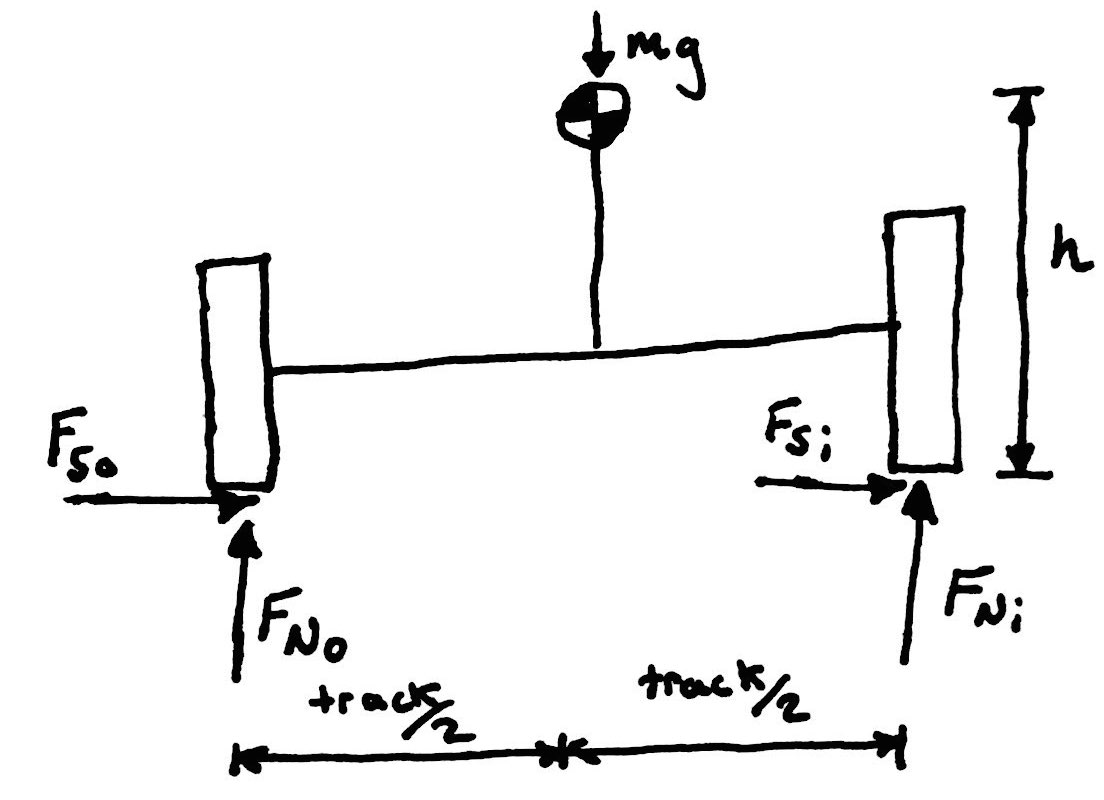
\includegraphics[width=.5\textwidth]{figures/cornering-fbd.jpg}
\caption{Free body diagram of vehicle cornering}
\label{fig:cornering-fbd}
\end{figure}

Using the half car model shown if Figure \ref{fig:cornering-fbd}, summing the moments about the centre of gravity and the vertical forces results in the following equations: 
\begin{gather}
\frac{1}{2}L_\mathrm{track}F_\mathrm{No} = hF_\mathrm{steer} + \frac{1}{2}L_\mathrm{track}F_\mathrm{Ni} \\
F_\mathrm{No} + F_\mathrm{Ni} = Mg
\end{gather}
Solving for the outside wheel normal force: 
\begin{equation}
\begin{split}
\frac{1}{2}L_\mathrm{track}F_\mathrm{No} &= hF_\mathrm{steer} + \frac{1}{2}L_\mathrm{track}(Mg - F_\mathrm{Ni})\\
F_\mathrm{No} &= \frac{hF_\mathrm{steer} + \frac{1}{2}L_\mathrm{track}Mg}{L_\mathrm{track}} = \frac{(\SI{0.52}{\metre})(\SI{5.43}{\kilo\newton})+(\SI{0.80}{\metre})(\SI{550}{\kilo\gram})\left(\SI{9.81}{\metre\per\second\squared}\right)}{\SI{1.60}{\metre}} = \SI{4.46}{\kilo\newton}
\end{split}
\end{equation}
Solving for the inside wheel normal force: 
\begin{equation}
F_\mathrm{Ni} = Mg - F_\mathrm{No} = (\SI{550}{\kilo\gram})\left(\SI{9.81}{\metre\per\second\squared}\right) - \SI{4.46}{\kilo\newton} = \SI{0.93}{\kilo\newton}
\end{equation}
Note that the forces above are for both front and rear outside wheels. Assuming the force is evenly split between the front and rear, there is approximately \SI{2.23}{\kilo\newton} of normal force on each outside tire and \SI{0.47}{\kilo\newton} for each inside tire during maximum cornering.
 
\subsection{Bump}
As stipulated in the ASC 2018 regulations, the analysis for suspension and steering must include loading considerations for a 2G bump. We interpret this requirement as the body of the vehicle accelerating upwards at 2G, in which case the additional normal force subjected to a single tire can be expressed as follows: 

\begin{equation}
F_\mathrm{N,bump} = \frac{2Mg}{4} = \frac{2(\SI{9.81}{\metre\per\second\squared})(\SI{550}{\kilo\gram})}{4} = \SI{2.70}{\kilo\newton}
\end{equation} 
 
\subsection{Superposition}
The braking, accelerating, and cornering conditions subject the wheels to normal forces that differ from those experienced when the car is at rest. The change in normal force for each loading condition can be expressed as follows: 
\begin{align}
\Delta F_\mathrm{Nf,braking}      &= F_\mathrm{Nf,braking}   - \frac{Mg}{4} =  \SI{1.87}{\kilo\newton} - \SI{1.35}{\kilo\newton} =  \SI{0.52}{\kilo\newton} \\
\Delta F_\mathrm{Nr,accelerating} &= F_\mathrm{Nf,braking}   - \frac{Mg}{4} =  \SI{1.47}{\kilo\newton} - \SI{1.35}{\kilo\newton} =  \SI{0.12}{\kilo\newton} \\
\Delta F_\mathrm{No,cornering}    &= F_\mathrm{No,cornering} - \frac{Mg}{4} =  \SI{2.23}{\kilo\newton} - \SI{1.35}{\kilo\newton} =  \SI{0.88}{\kilo\newton} \\
\Delta F_\mathrm{Ni,cornering}    &= F_\mathrm{No,cornering} - \frac{Mg}{4} =  \SI{0.47}{\kilo\newton} - \SI{1.35}{\kilo\newton} = -\SI{0.88}{\kilo\newton} \\
\Delta F_\mathrm{N,bump}          &= F_\mathrm{N,bump}       - \frac{Mg}{4} =  \SI{2.70}{\kilo\newton} - \SI{1.35}{\kilo\newton} =  \SI{1.35}{\kilo\newton}
\end{align}
To approximate the worst case loading condition, a superposition of the changes in normal force and the nominal normal force is applied. Note that the nominal force used is the same for each wheel, which assumes a centre of gravity approximately centred along the wheelbase.
\begin{align}
F_\mathrm{Nfi,max} &= \Delta F_\mathrm{Nf,braking} + \Delta F_\mathrm{Ni,cornering} + 2F_\mathrm{N,nominal} = \SI{0.52}{\kilo\newton} - \SI{0.88}{\kilo\newton} + \SI{2.70}{\kilo\newton} = \SI{2.34}{\kilo\newton} \\
F_\mathrm{Nfo,max} &= \Delta F_\mathrm{Nf,braking} + \Delta F_\mathrm{No,cornering} + 2F_\mathrm{N,nominal} = \SI{0.52}{\kilo\newton} + \SI{0.88}{\kilo\newton} + \SI{2.70}{\kilo\newton} = \SI{4.10}{\kilo\newton} \\
F_\mathrm{Nri,max} &= \Delta F_\mathrm{Nr,braking} + \Delta F_\mathrm{Ni,cornering} + 2F_\mathrm{N,nominal} = \SI{0.12}{\kilo\newton} - \SI{0.88}{\kilo\newton} + \SI{2.70}{\kilo\newton} = \SI{1.94}{\kilo\newton} \\
F_\mathrm{Nro,max} &= \Delta F_\mathrm{Nr,braking} + \Delta F_\mathrm{No,cornering} + 2F_\mathrm{N,nominal} = \SI{0.12}{\kilo\newton} + \SI{0.88}{\kilo\newton} + \SI{2.70}{\kilo\newton} = \SI{3.70}{\kilo\newton} 
\end{align}

\subsection{Summary}
Table \ref{tab:worst-case-loading} summarizes the loading conditions used for static structural FEA simulations on the suspension and steering components. Note that the direction of the force corresponds's with the global coordinate system of the MSXII and the vectors shown in Figure \ref{fig:suspension-coordinate-system}. The assemblies shown are for the driver's side of the vehicle

\begin{table}[h!]
\centering
\caption{Summary of worst case loading conditions}
\label{tab:worst-case-loading}
\begin{tabular}{lrrr}
\toprule
Worst Case Loading                             & $F_x$ (\si{\kilo\newton}) & $F_y$ (\si{\kilo\newton}) & $F_z$ (\si{\kilo\newton}) \\
\midrule
Braking \& Cornering (Inside Front Wheel)      & 2.72                     & 2.34                     & 2.70                     \\
Braking \& Cornering (Outside Front Wheel)     & -2.72                    & 4.10                     & 2.70                     \\
Accelerating \& Cornering (Inside Rear Wheel)  & 2.72                     & 1.94                     & 0.99                     \\
Accelerating \& Cornering (Outside Rear Wheel) & -2.72                    & 3.70                     & 0.99                     \\
\bottomrule
\end{tabular}
\end{table}

\begin{figure}
\centering
\begin{subfigure}[b]{.48\textwidth}
\centering
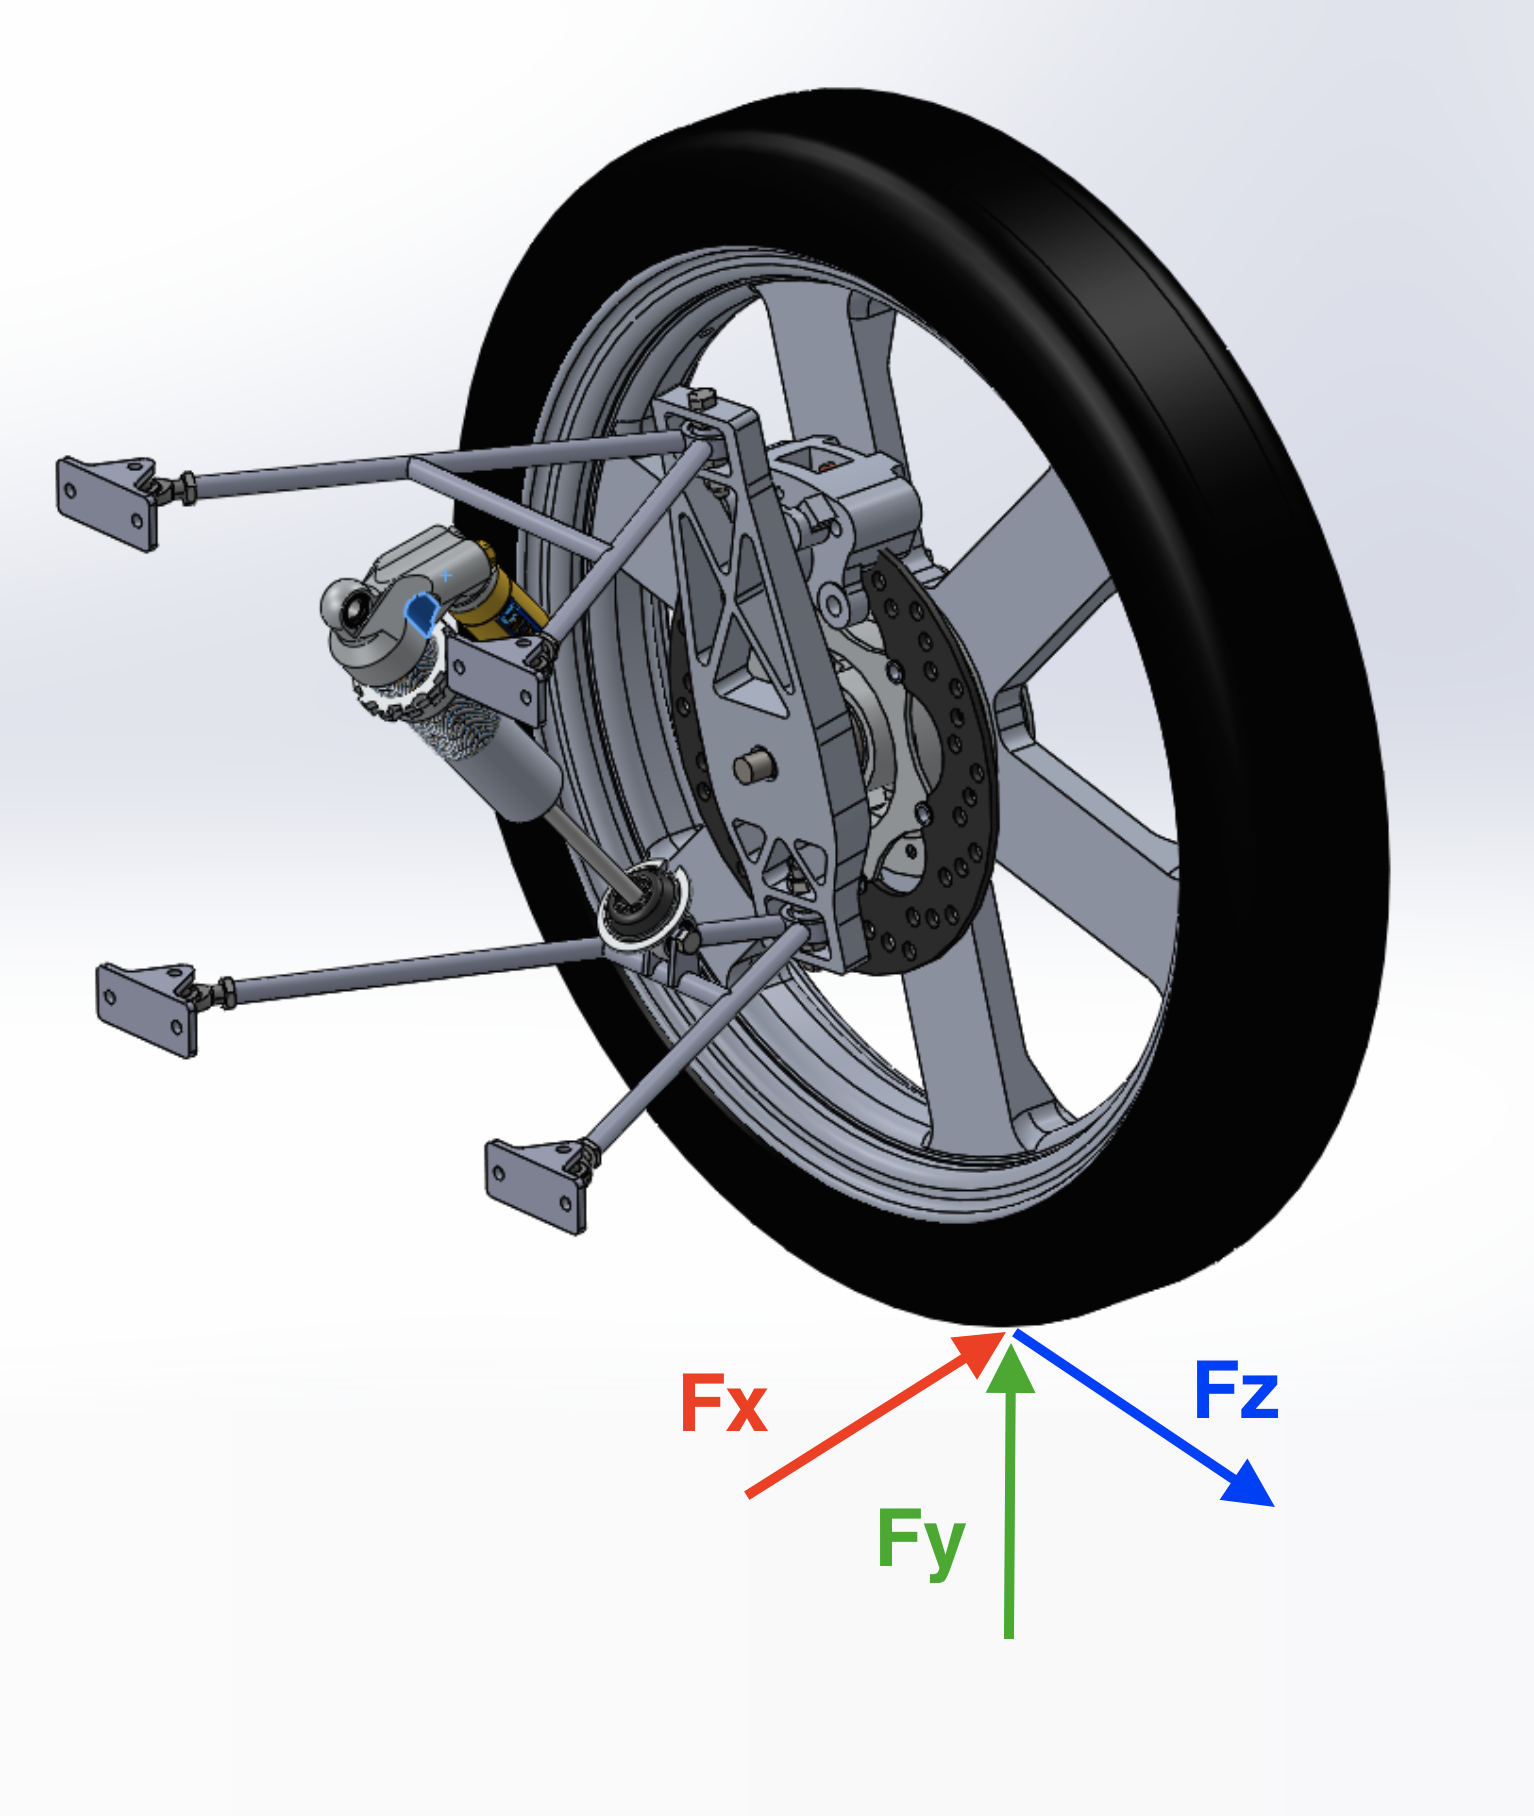
\includegraphics[width=0.9\textwidth]{figures/front-axis-directions}
\caption{Font suspension}
\end{subfigure}
\begin{subfigure}[b]{.48\textwidth}
\centering
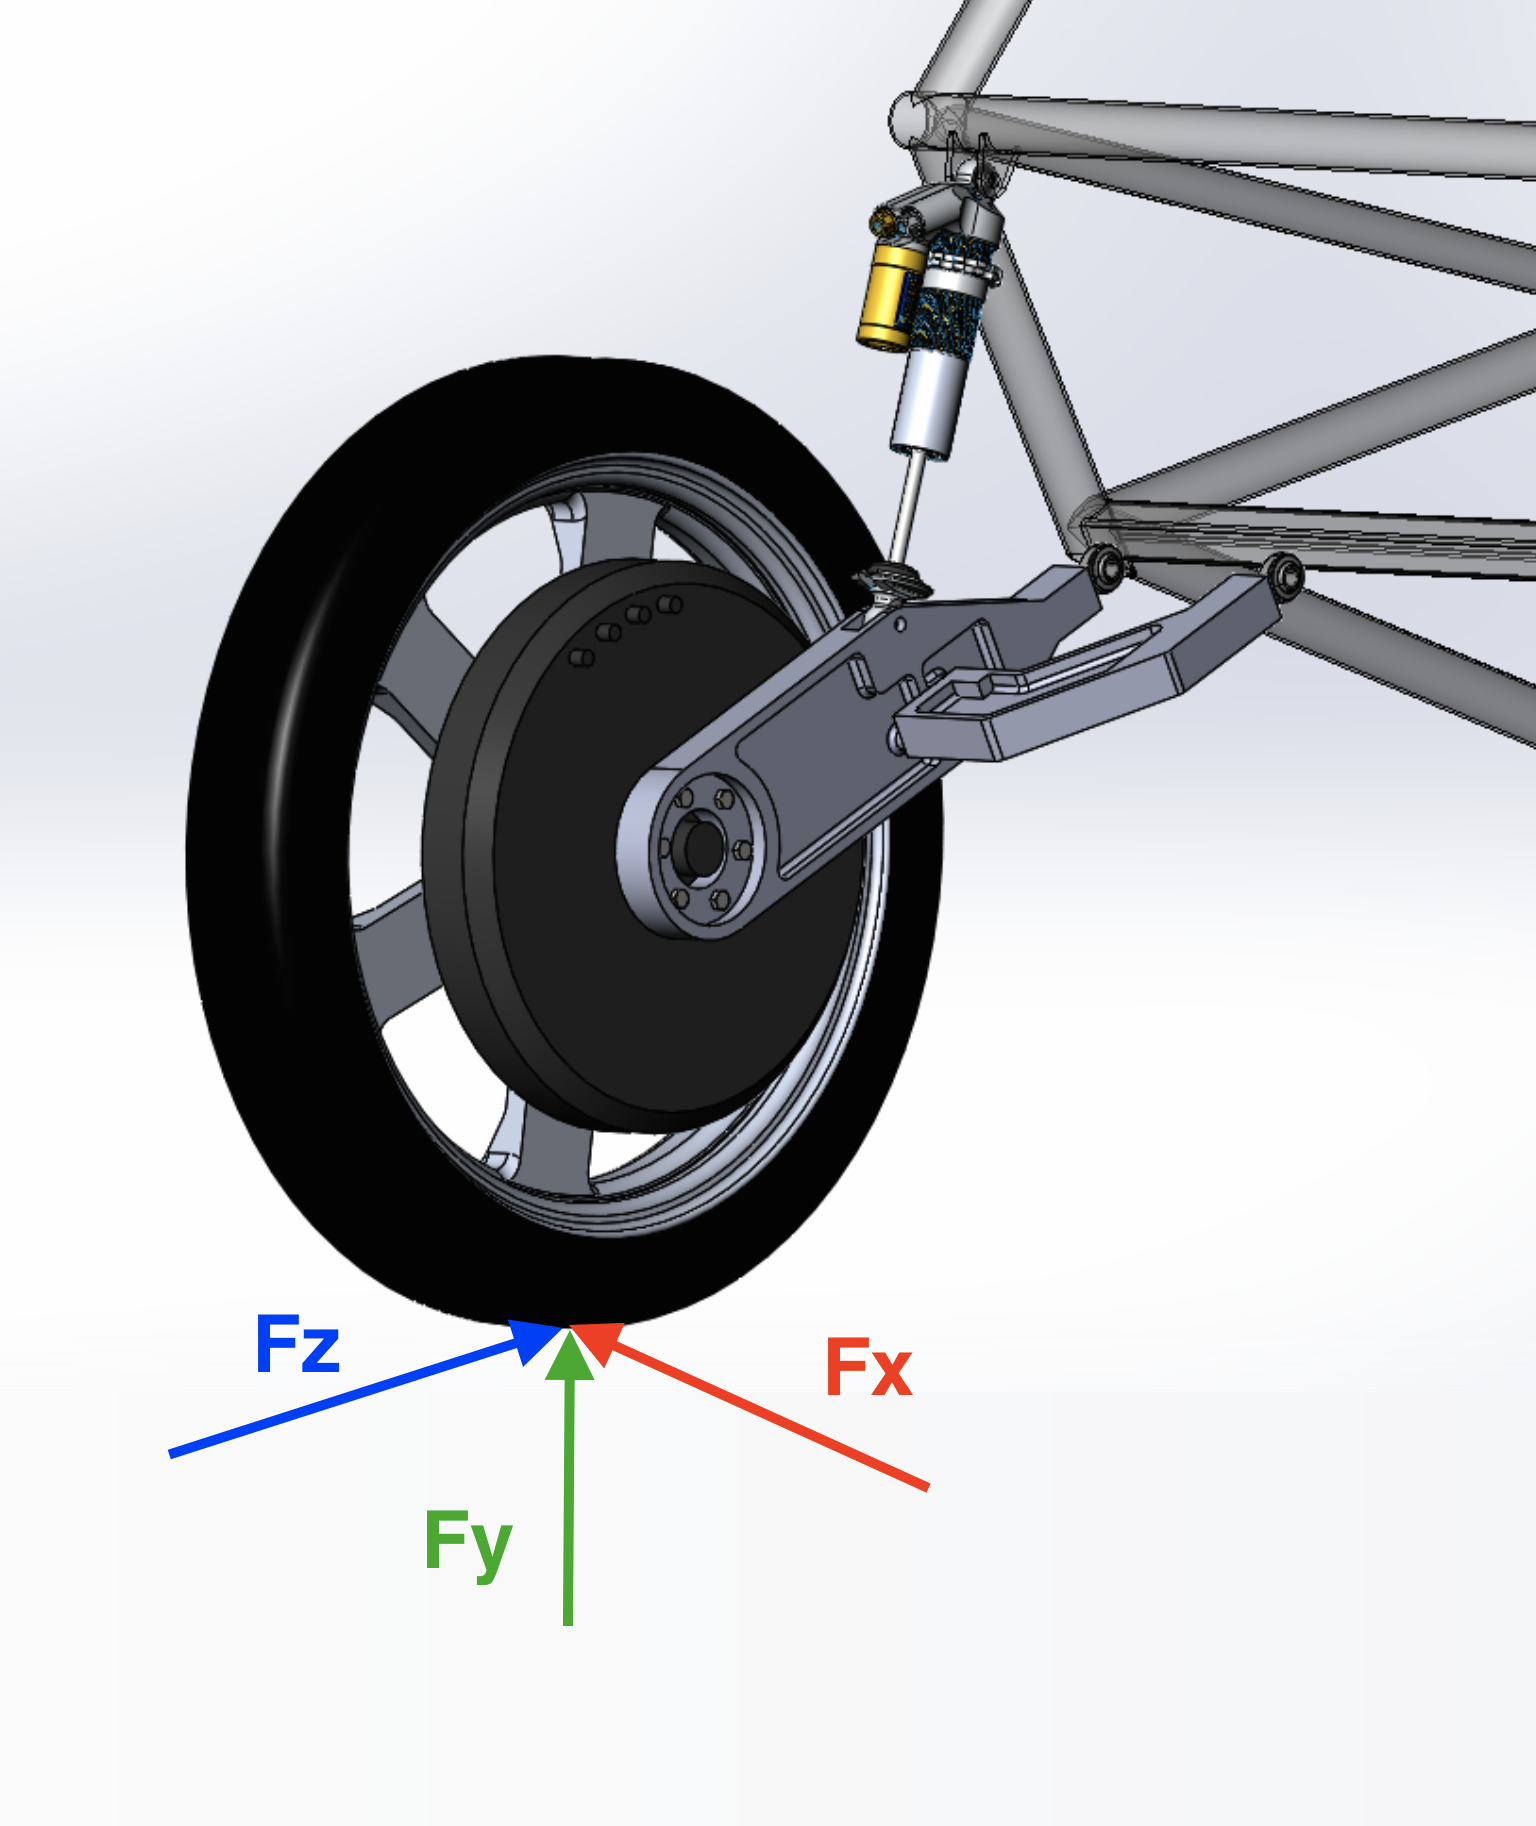
\includegraphics[width=0.9\textwidth]{figures/rear-axis-directions}
\caption{Rear suspenion}
\end{subfigure}
\caption{Suspension coordinate system}
\label{fig:suspension-coordinate-system}
\end{figure}

\clearpage
\section{FEA images for chassis}
\label{sec:fea-chassis-images}

\begin{figure}[H]
\centering
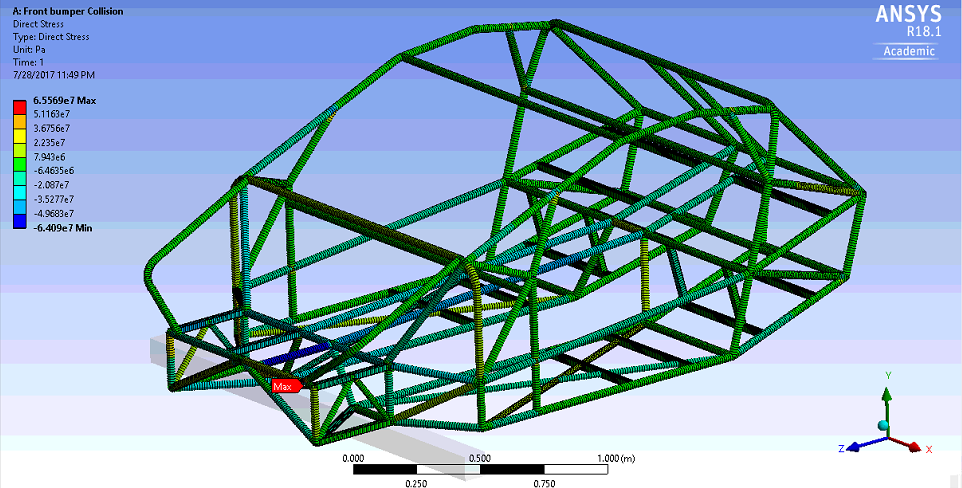
\includegraphics[width=0.5\textwidth]{figures/fea/chassis/chassis-collision-bumper-front}
\caption{Front bumper collision}
\label{sec:chassis-collision-bumper-front}
\end{figure}

\begin{figure}[H]
\centering
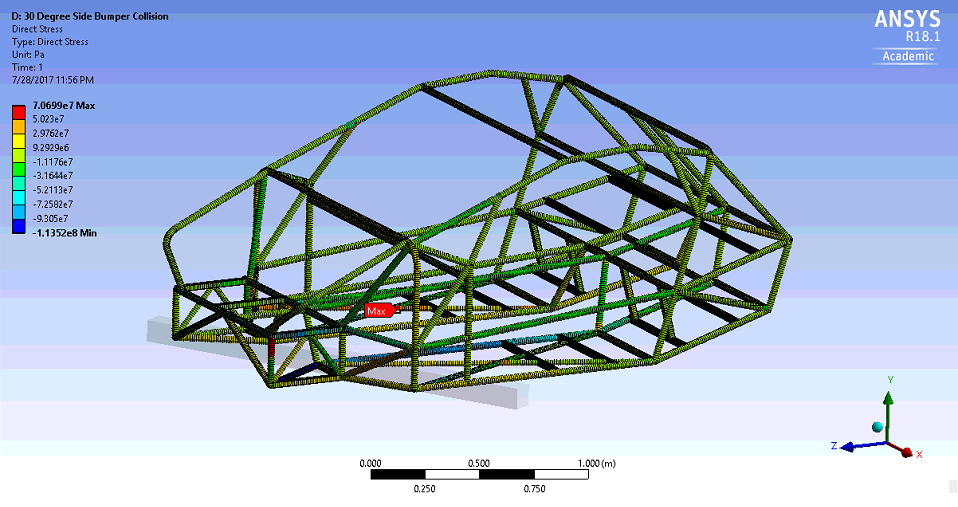
\includegraphics[width=0.5\textwidth]{figures/fea/chassis/chassis-collision-bumper-30deg}
\caption{Front bumper 30 degree collision}
\label{sec:chassis-collision-bumper-30deg}
\end{figure}

\begin{figure}[H]
\centering
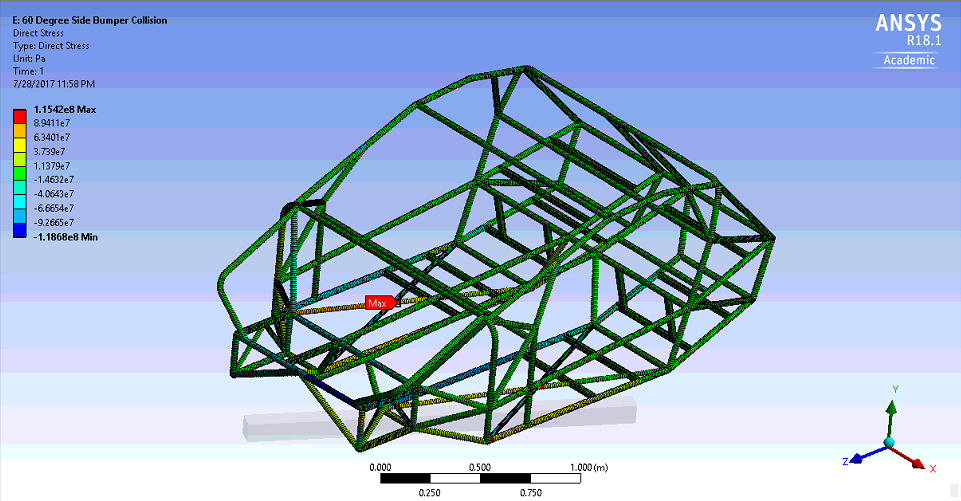
\includegraphics[width=0.5\textwidth]{figures/fea/chassis/chassis-collision-bumper-60deg}
\caption{Front bumper 60 degree collision}
\label{sec:chassis-collision-bumper-60deg}
\end{figure}

\begin{figure}[H]
\centering
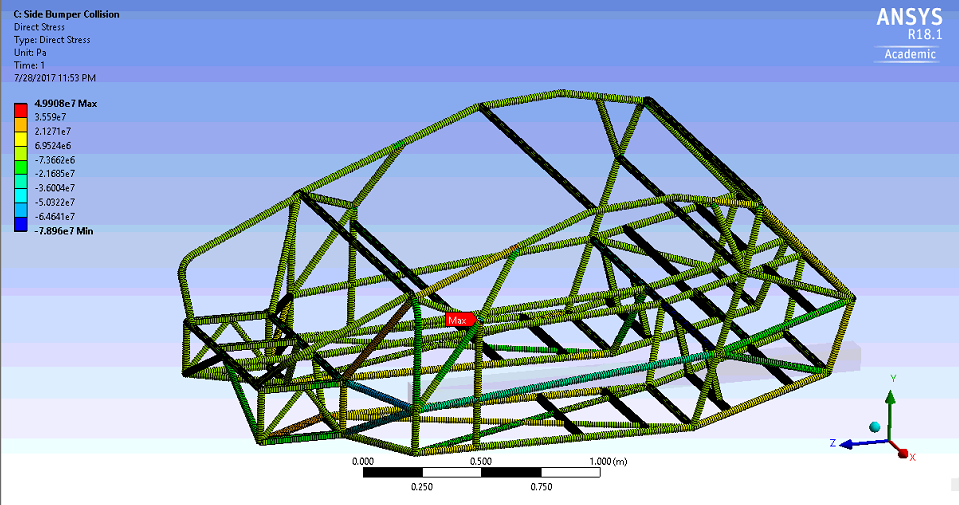
\includegraphics[width=0.5\textwidth]{figures/fea/chassis/chassis-collision-bumper-side}
\caption{Side bumper collision}
\label{sec:chassis-collision-bumper-side}
\end{figure}

\begin{figure}[H]
\centering
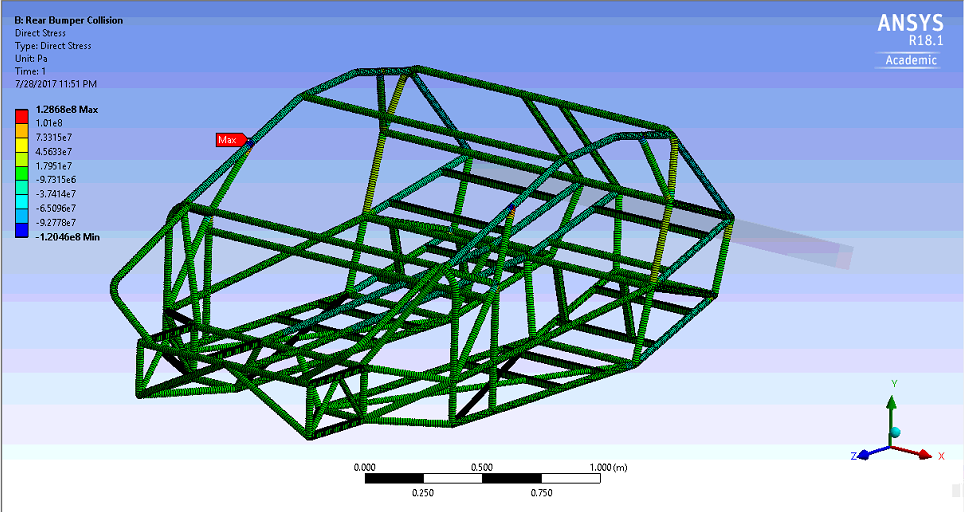
\includegraphics[width=0.5\textwidth]{figures/fea/chassis/chassis-collision-bumper-rear}
\caption{Rear bumper collision}
\label{sec:chassis-collision-bumper-rear}
\end{figure}

\begin{figure}[H]
\centering
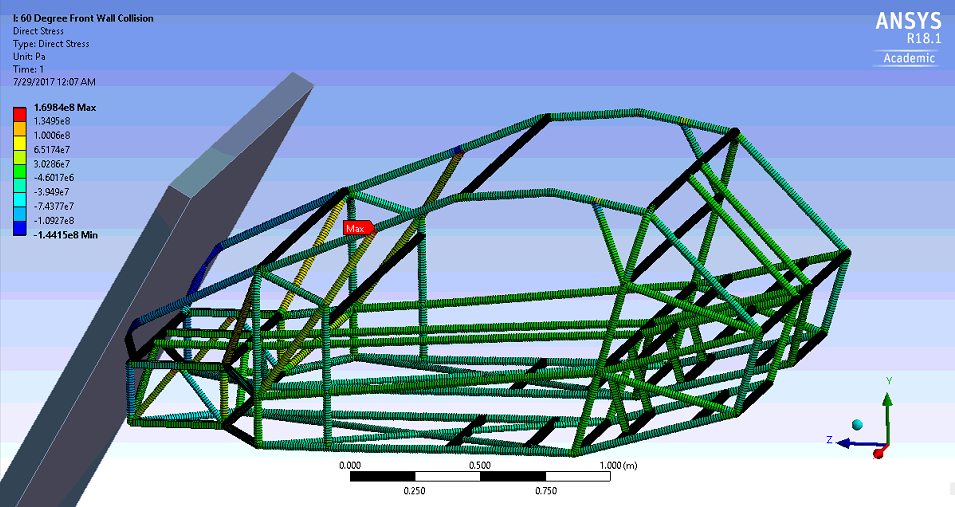
\includegraphics[width=0.5\textwidth]{figures/fea/chassis/chassis-collision-hood-60deg}
\caption{Hood 60 degree collision}
\label{sec:chassis-collision-hood-60deg}
\end{figure}

\begin{figure}[H]
\centering
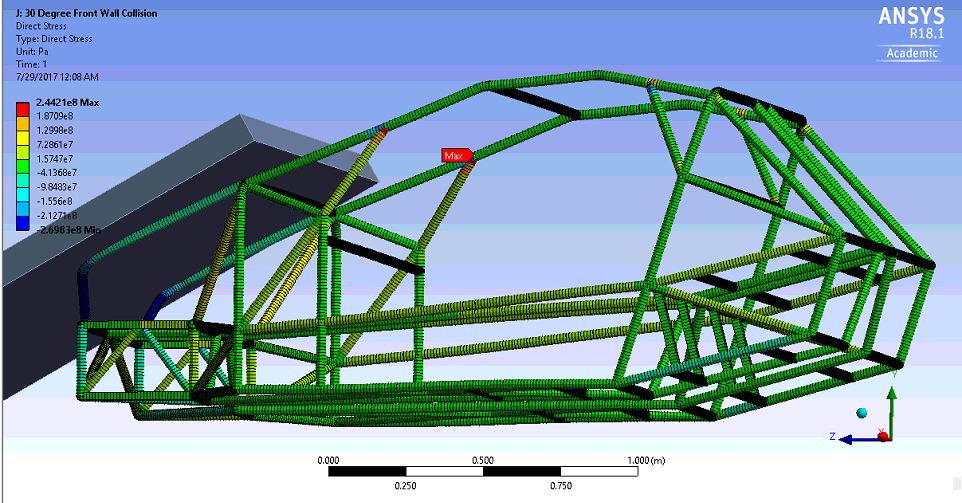
\includegraphics[width=0.5\textwidth]{figures/fea/chassis/chassis-collision-hood-30deg}
\caption{Hood 30 degree collision}
\label{sec:chassis-collision-hood-30deg}
\end{figure}

\begin{figure}[H]
\centering
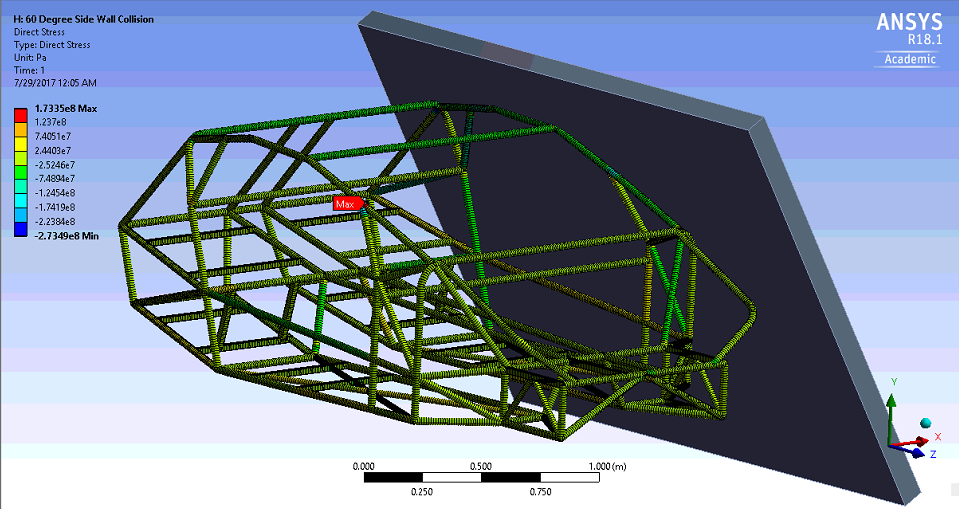
\includegraphics[width=0.5\textwidth]{figures/fea/chassis/chassis-collision-side-60deg}
\caption{Side 60 degree collision}
\label{sec:chassis-collision-side-60deg}
\end{figure}

\begin{figure}[H]
\centering
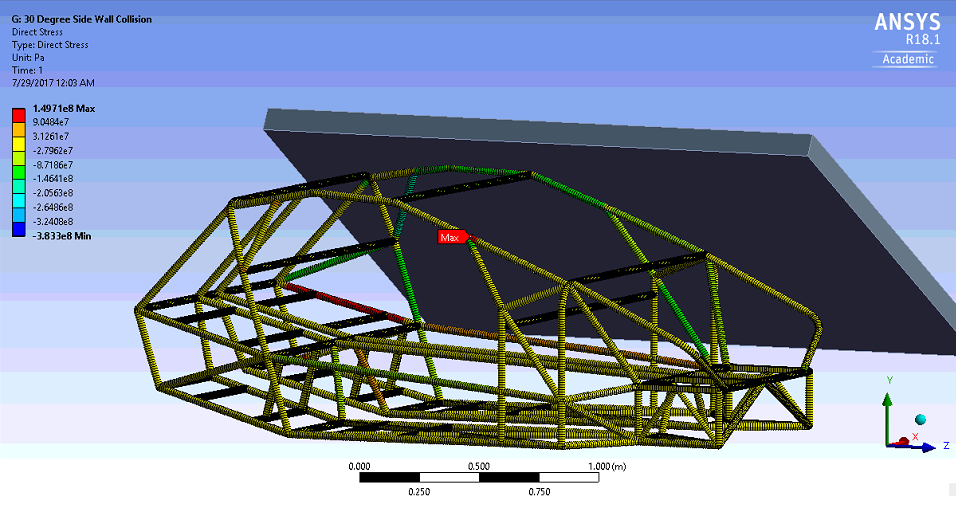
\includegraphics[width=0.5\textwidth]{figures/fea/chassis/chassis-collision-side-30deg}
\caption{Side 30 degree collision}
\label{sec:chassis-collision-side-30deg}
\end{figure}

\begin{figure}[H]
\centering
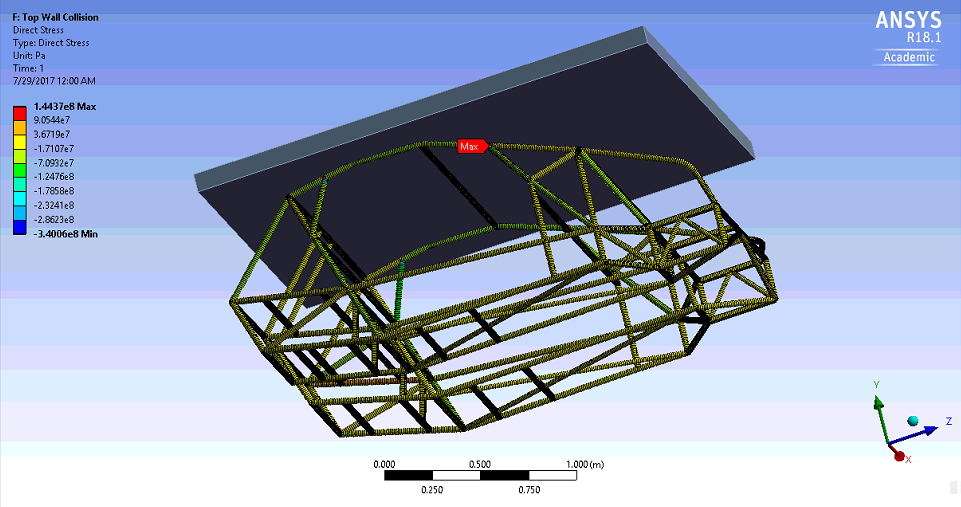
\includegraphics[width=0.5\textwidth]{figures/fea/chassis/chassis-collision-top}
\caption{Roof top collision}
\label{sec:chassis-collision-top}
\end{figure}

\begin{figure}[H]
\centering
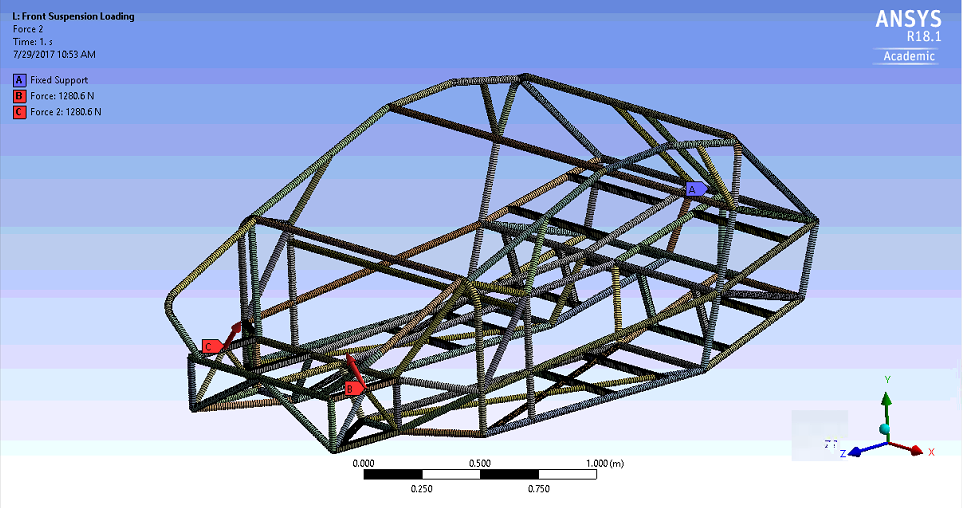
\includegraphics[width=0.5\textwidth]{figures/fea/chassis/chassis-front-suspension-rest-loading}
\caption{Vehicle rest front subframe loading}
\label{sec:chassis-front-suspension-rest-loading}
\end{figure}

\begin{figure}[H]
\centering
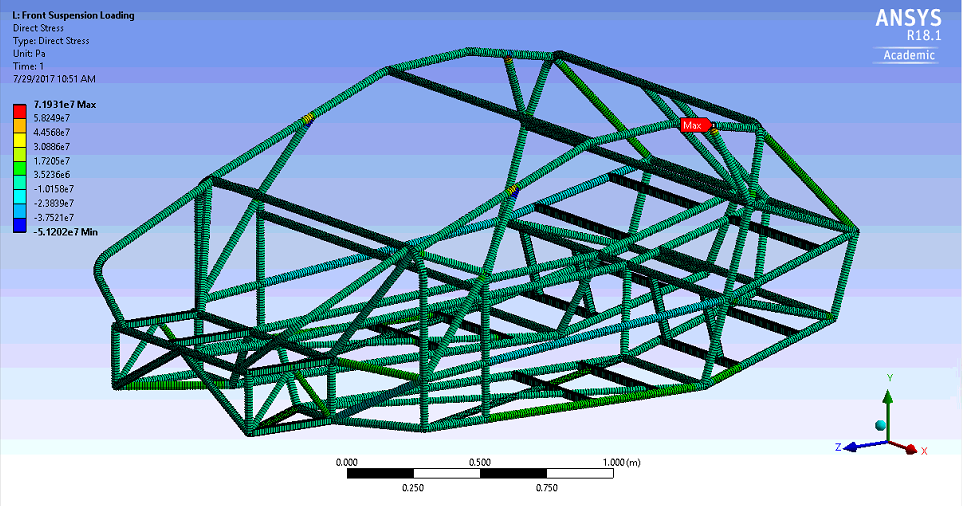
\includegraphics[width=0.5\textwidth]{figures/fea/chassis/chassis-front-suspension-stress}
\caption{Vehicle rest front subframe stress}
\label{sec:chassis-front-suspension-stress}
\end{figure}

\begin{figure}[H]
\centering
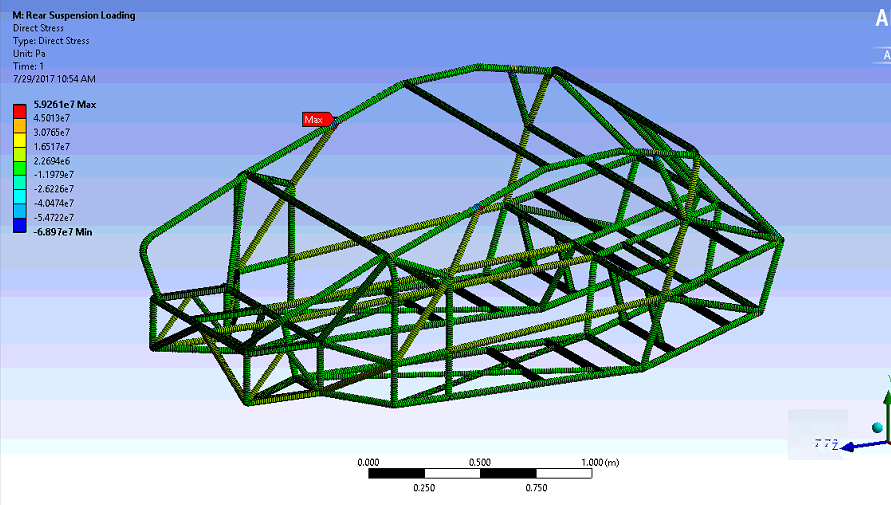
\includegraphics[width=0.5\textwidth]{figures/fea/chassis/chassis-rear-suspension-stress}
\caption{Vehicle rest rear subframe stress}
\label{sec:chassis-rear-suspension-stress}
\end{figure}

\begin{figure}[H]
\centering
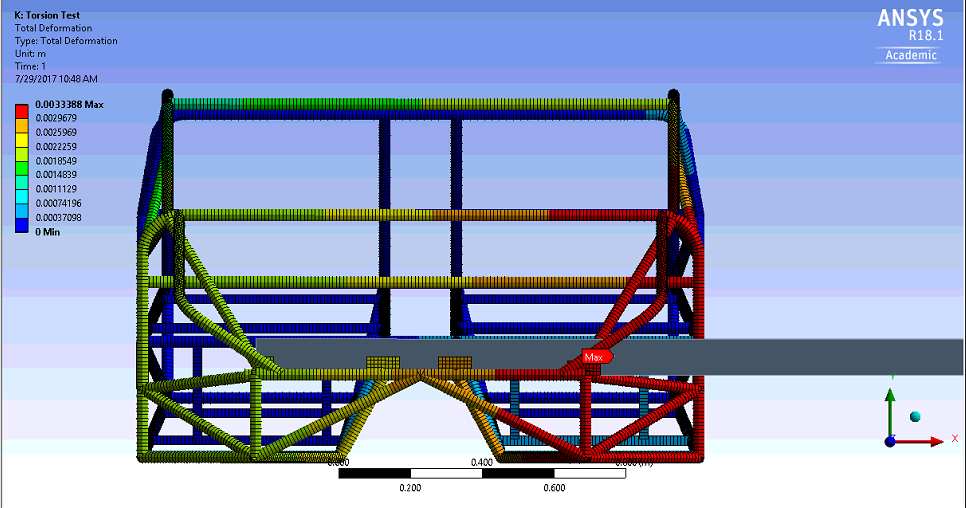
\includegraphics[width=0.5\textwidth]{figures/fea/chassis/torsion-deformation}
\caption{Torsion test, deformation}
\label{sec:torsion-deformation}
\end{figure}

\begin{figure}[H]
\centering
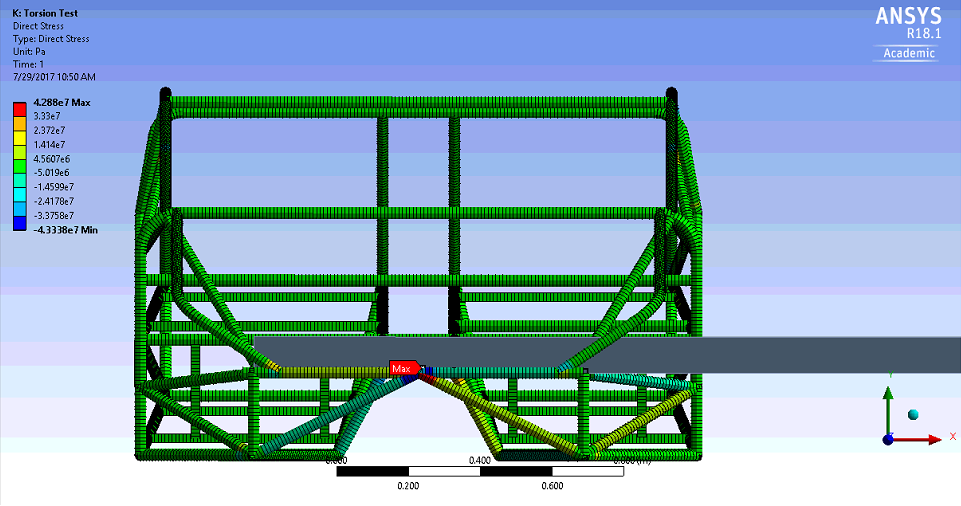
\includegraphics[width=0.5\textwidth]{figures/fea/chassis/torsion-stress}
\caption{Torsion test, stress}
\label{sec:torsion-stress}
\end{figure}

\clearpage
\section{FEA images for suspension and steering}
\label{sec:fea-parts-images}

\begin{figure}[H]
\centering
\begin{subfigure}[b]{.48\textwidth}
\centering
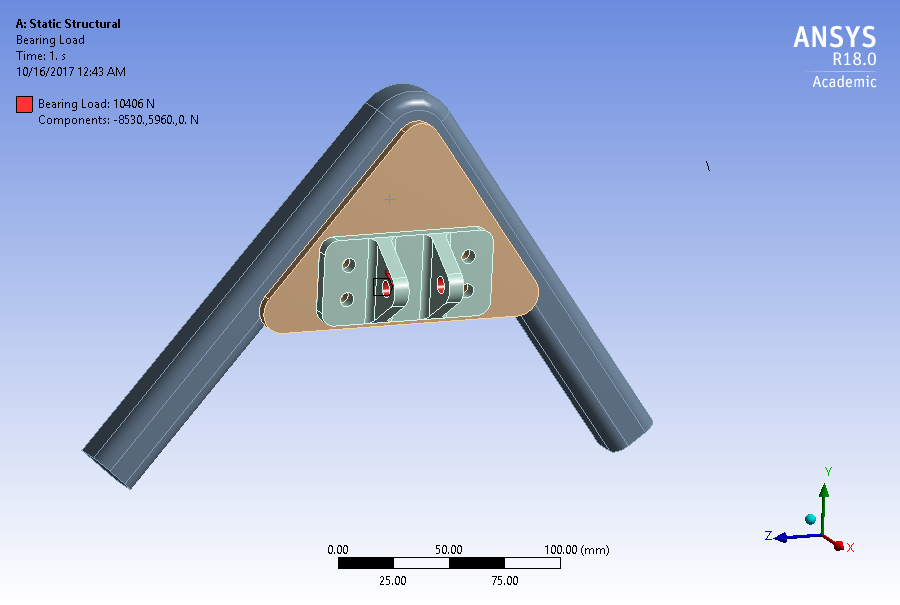
\includegraphics[width=0.9\textwidth]{figures/fea/parts/MS00015-CoiloverClevis-Setup}
\caption{Setup}
\end{subfigure}
\begin{subfigure}[b]{.48\textwidth}
\centering
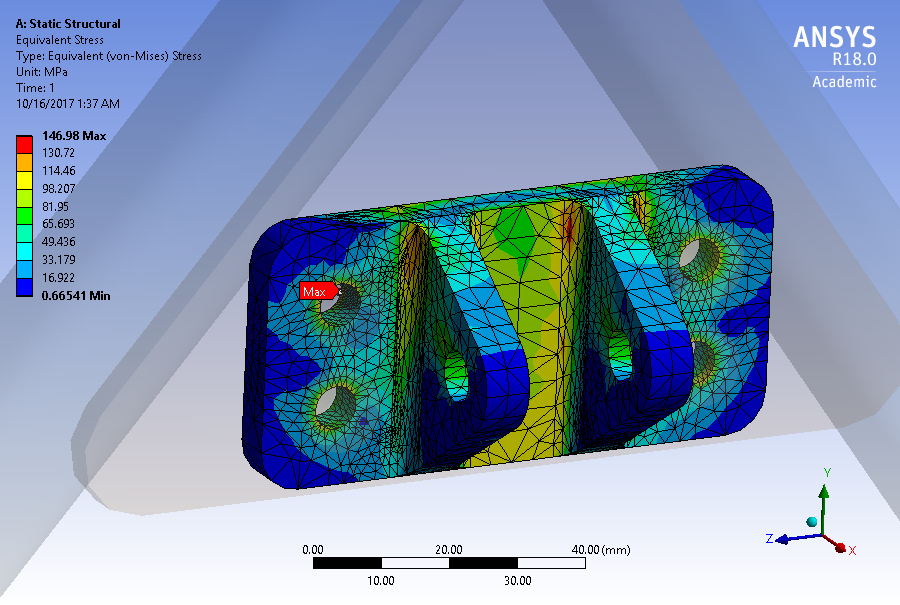
\includegraphics[width=0.9\textwidth]{figures/fea/parts/MS00015-CoiloverClevis-Stress}
\caption{Stress}
\end{subfigure}
\caption{Coilover clevis}
\label{fig:MS00015-CoiloverClevis}
\end{figure}

\begin{figure}[H]
\centering
\begin{subfigure}[b]{.48\textwidth}
\centering
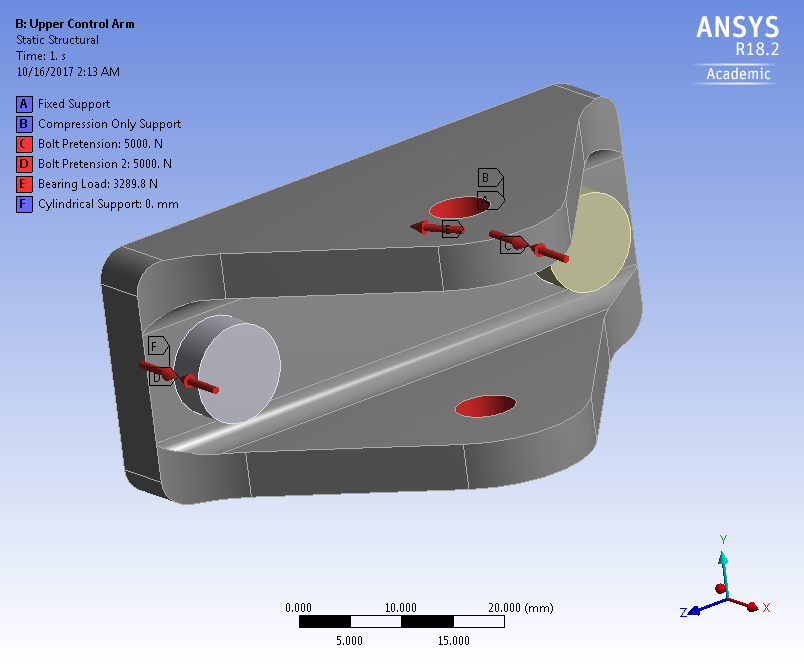
\includegraphics[width=0.9\textwidth]{figures/fea/parts/MS00029-UpperControlArmClevis-Setup}
\caption{Setup}
\end{subfigure}
\begin{subfigure}[b]{.48\textwidth}
\centering
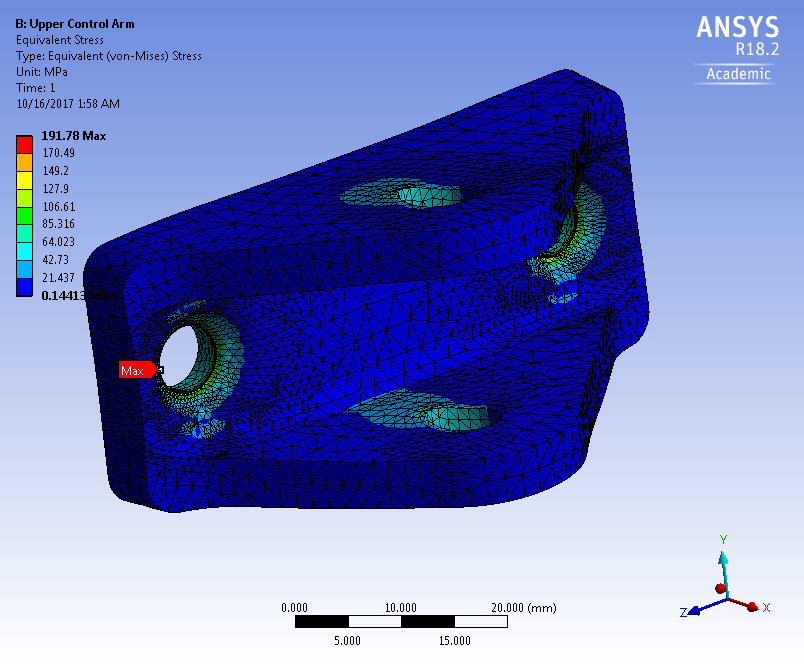
\includegraphics[width=0.9\textwidth]{figures/fea/parts/MS00029-UpperControlArmClevis-Stress}
\caption{Stress}
\end{subfigure}
\caption{Upper control arm clevis}
\label{fig:MS00029-UpperControlArmClevis}
\end{figure}

\begin{figure}[H]
\centering
\begin{subfigure}[b]{.48\textwidth}
\centering
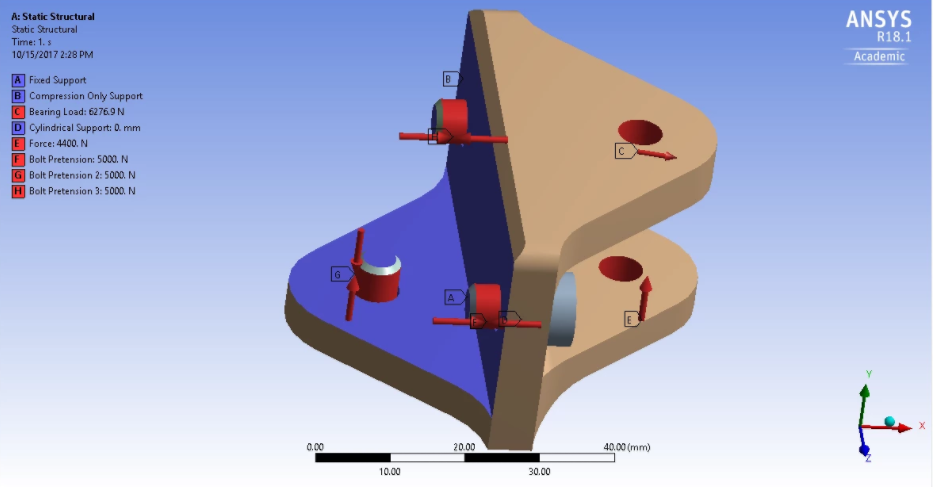
\includegraphics[width=0.9\textwidth]{figures/fea/parts/MS00102-LowerControlArmClevis-Setup}
\caption{Setup}
\end{subfigure}
\begin{subfigure}[b]{.48\textwidth}
\centering
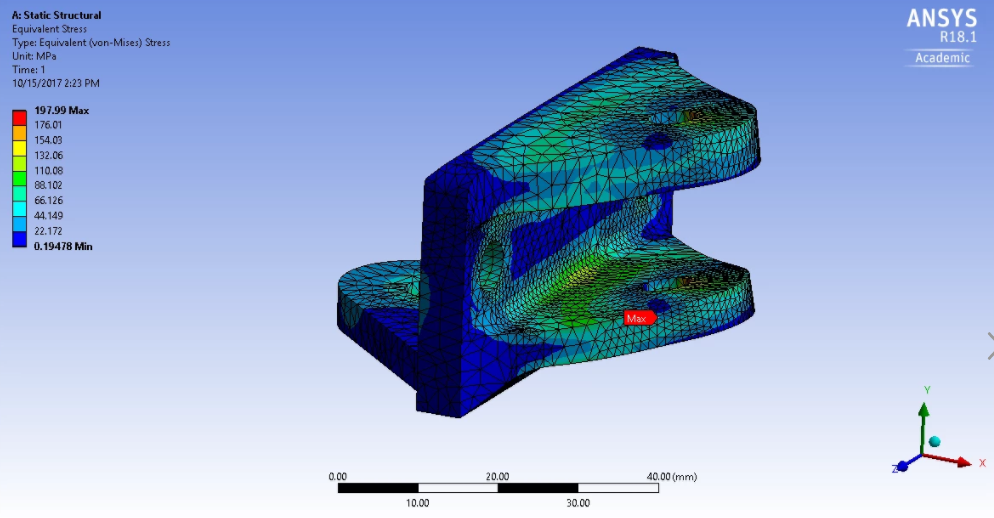
\includegraphics[width=0.9\textwidth]{figures/fea/parts/MS00102-LowerControlArmClevis-Stress}
\caption{Stress}
\end{subfigure}
\caption{Lower control arm clevis}
\label{fig:MS00102-LowerControlArmClevis}
\end{figure}

\begin{figure}[H]
\centering
\begin{subfigure}[b]{.48\textwidth}
\centering
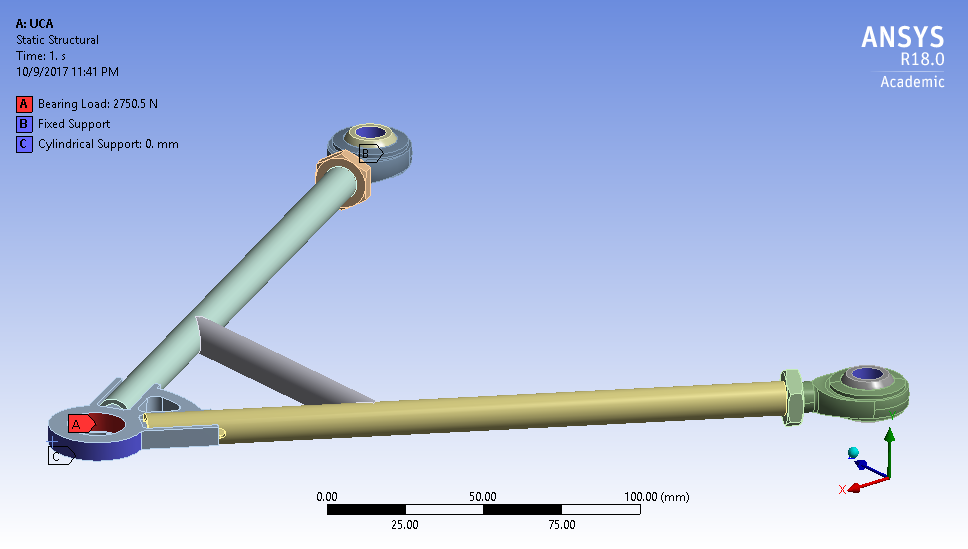
\includegraphics[width=0.9\textwidth]{figures/fea/parts/MS00017-UpperControlArm-Setup}
\caption{Setup}
\end{subfigure}
\begin{subfigure}[b]{.48\textwidth}
\centering
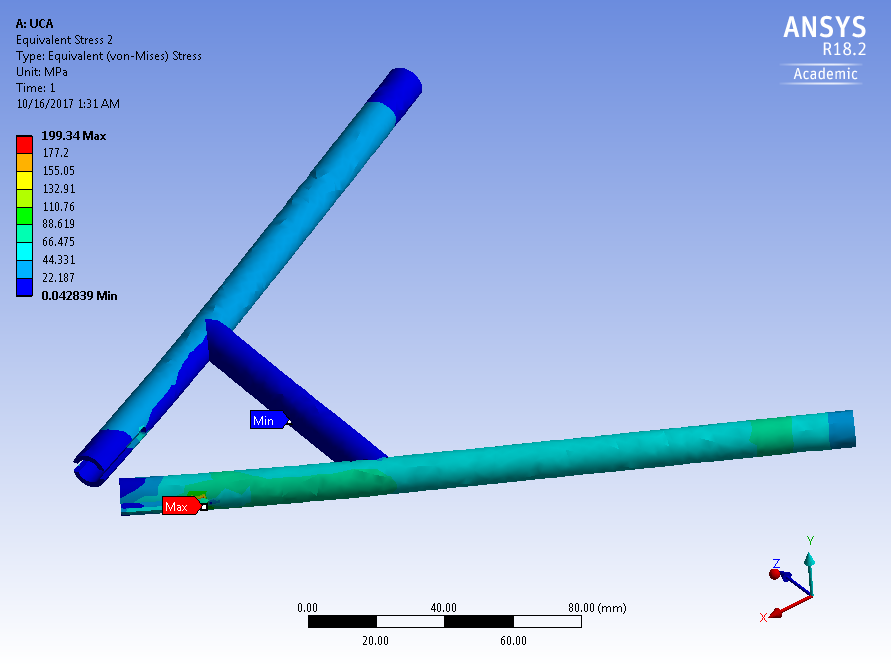
\includegraphics[width=0.9\textwidth]{figures/fea/parts/MS00017-UpperControlArm-Stress}
\caption{Stress}
\end{subfigure}
\caption{Upper control arm}
\label{fig:MS00017-UpperControlArm}
\end{figure}

\begin{figure}[H]
\centering
\begin{subfigure}[b]{.48\textwidth}
\centering
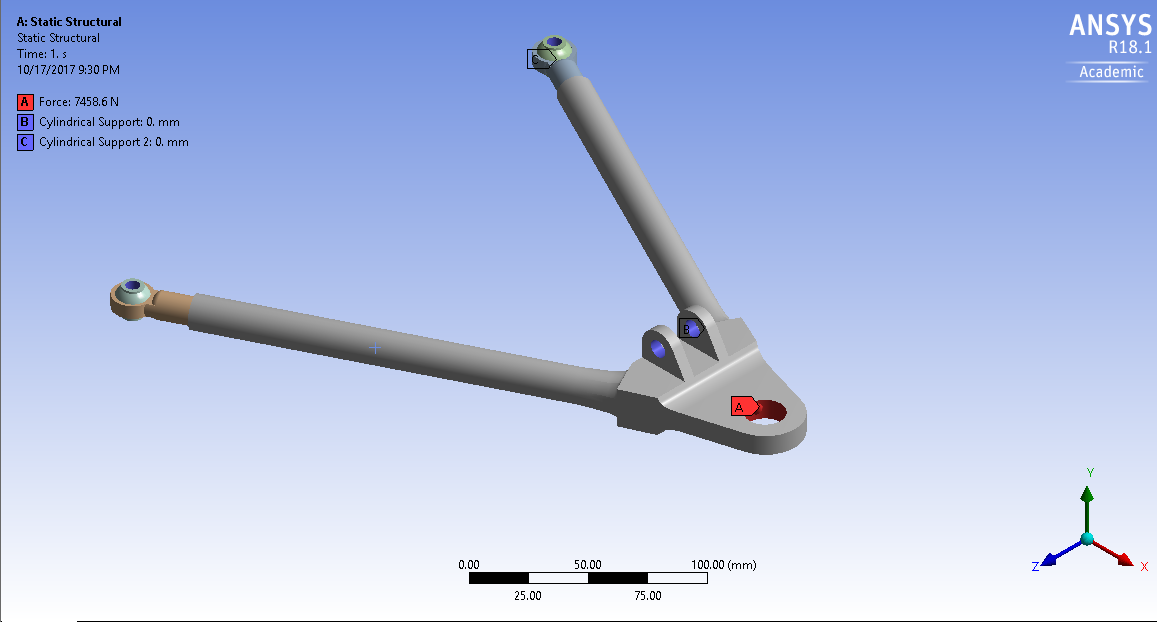
\includegraphics[width=0.9\textwidth]{figures/fea/parts/MS00018-LowerControlArm-Setup}
\caption{Setup}
\end{subfigure}
\begin{subfigure}[b]{.48\textwidth}
\centering
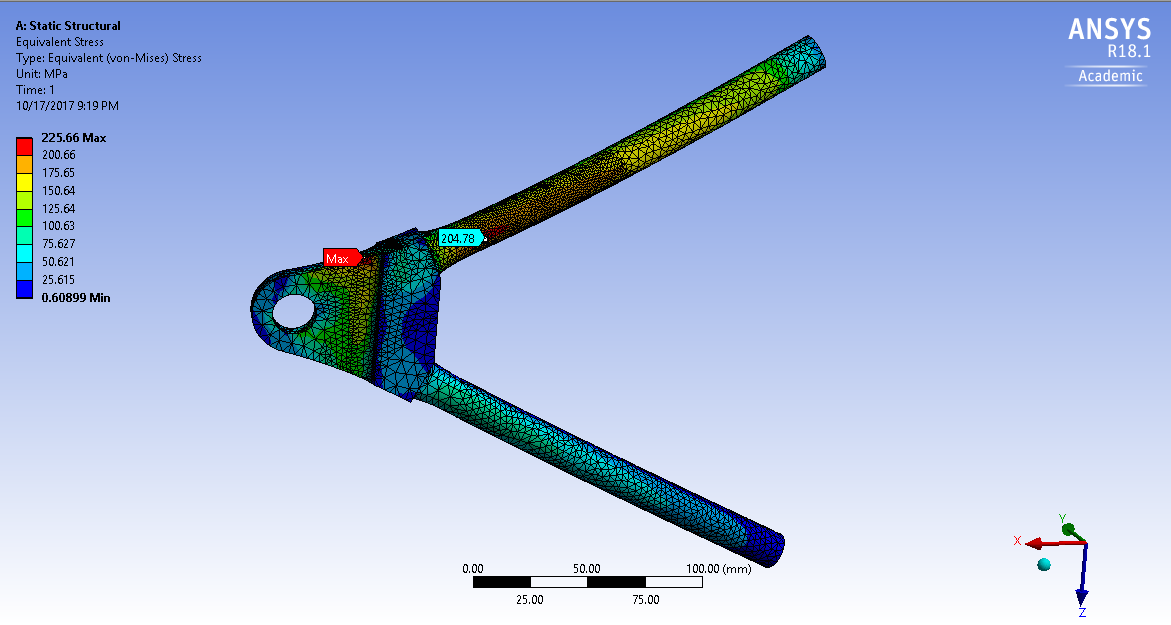
\includegraphics[width=0.9\textwidth]{figures/fea/parts/MS00018-LowerControlArm-Stress}
\caption{Stress}
\end{subfigure}
\caption{Lower control arm}
\label{fig:MS00018-LowerControlArm}
\end{figure}

\begin{figure}[H]
\centering
\begin{subfigure}[b]{.48\textwidth}
\centering
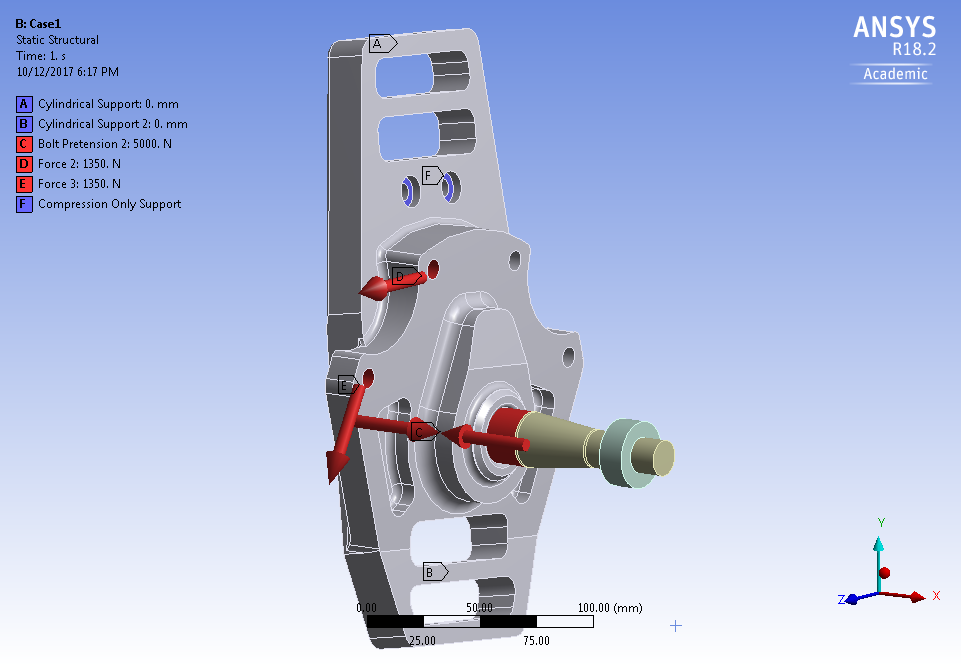
\includegraphics[width=0.9\textwidth]{figures/fea/parts/MS00019-Upright-Setup}
\caption{Setup}
\end{subfigure}
\begin{subfigure}[b]{.48\textwidth}
\centering
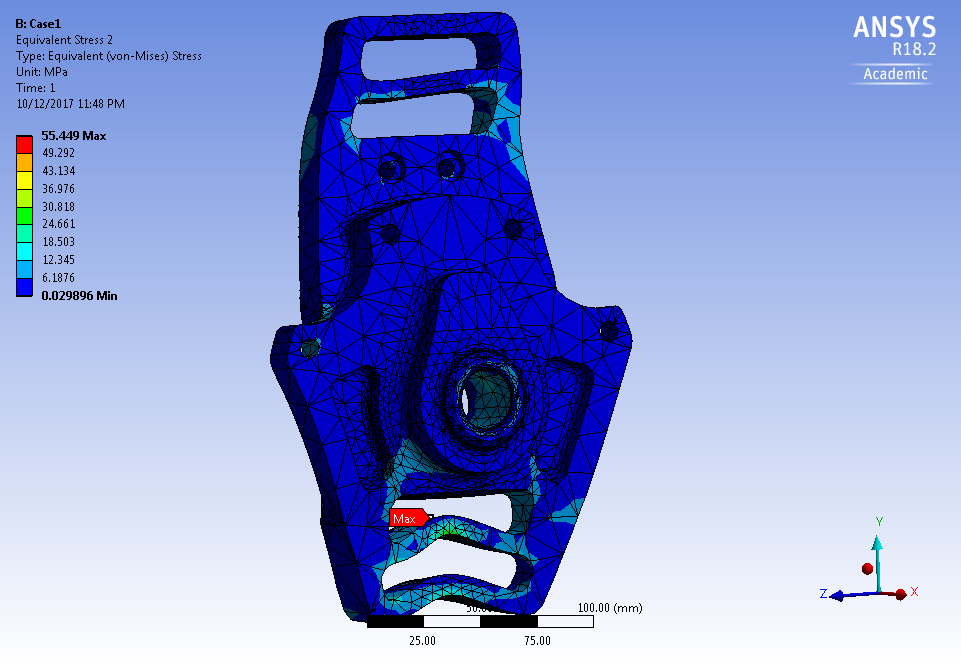
\includegraphics[width=0.9\textwidth]{figures/fea/parts/MS00019-Upright-Stress}
\caption{Stress}
\end{subfigure}
\caption{Upright}
\label{fig:MS00019-Upright}
\end{figure}

\begin{figure}[H]
\centering
\begin{subfigure}[b]{.48\textwidth}
\centering
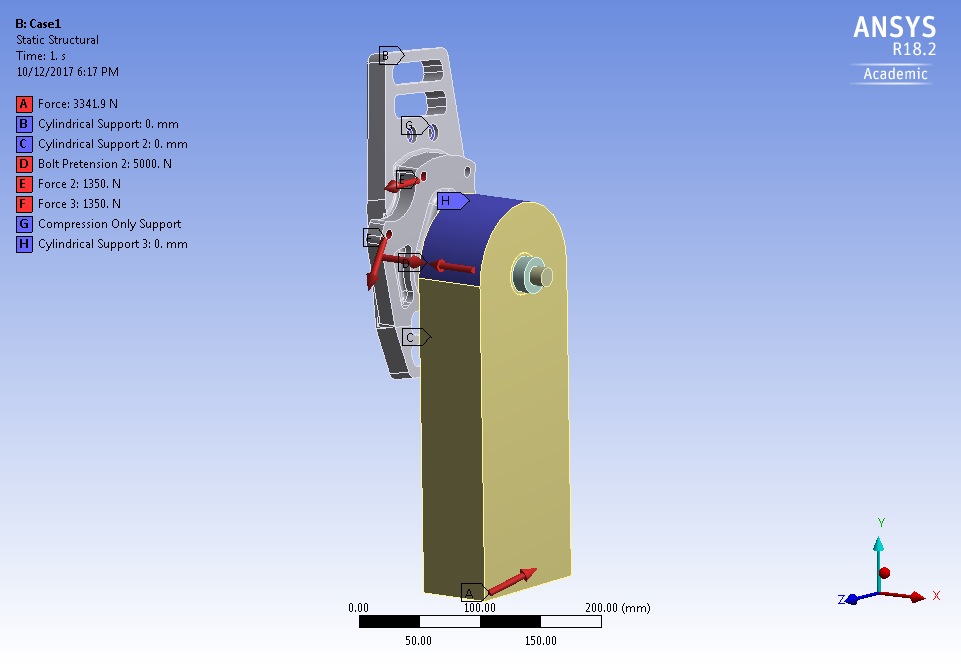
\includegraphics[width=0.9\textwidth]{figures/fea/parts/MS00020-Spindle-Setup}
\caption{Setup}
\end{subfigure}
\begin{subfigure}[b]{.48\textwidth}
\centering
\includegraphics[width=0.9\textwidth]{figures/fea/parts/MS00020-Spindle-Stress}
\caption{Stress}
\end{subfigure}
\caption{Spindle}
\label{fig:MS00020-Spindle}
\end{figure}

\begin{figure}[H]
\centering
\begin{subfigure}[b]{.48\textwidth}
\centering
\includegraphics[width=0.9\textwidth]{figures/fea/parts/MS00030-UpperBearingPlate-Setup}
\caption{Setup}
\end{subfigure}
\begin{subfigure}[b]{.48\textwidth}
\centering
\includegraphics[width=0.9\textwidth]{figures/fea/parts/MS00030-UpperBearingPlate-Stress}
\caption{Stress}
\end{subfigure}
\caption{Upper bearing plate}
\label{fig:MS00030-UpperBearingPlate}
\end{figure}

\begin{figure}[H]
\centering
\begin{subfigure}[b]{.48\textwidth}
\centering
\includegraphics[width=0.9\textwidth]{figures/fea/parts/MS00036-CoiloverControlArmTab-Setup}
\caption{Setup}
\end{subfigure}
\begin{subfigure}[b]{.48\textwidth}
\centering
\includegraphics[width=0.9\textwidth]{figures/fea/parts/MS00036-CoiloverControlArmTab-Stress}
\caption{Stress}
\end{subfigure}
\caption{Coilover control arm tab}
\label{fig:MS00036-CoiloverControlArmTab}
\end{figure}

\begin{figure}[H]
\centering
\begin{subfigure}[b]{.48\textwidth}
\centering
\includegraphics[width=0.9\textwidth]{figures/fea/parts/MS00038-CoiloverMountingPlate-Setup}
\caption{Setup}
\end{subfigure}
\begin{subfigure}[b]{.48\textwidth}
\centering
\includegraphics[width=0.9\textwidth]{figures/fea/parts/MS00038-CoiloverMountingPlate-Stress}
\caption{Stress}
\end{subfigure}
\caption{Coilover mounting plate}
\label{fig:MS00038-CoiloverMountingPlate}
\end{figure}

\begin{figure}[H]
\centering
\begin{subfigure}[b]{.48\textwidth}
\centering
\includegraphics[width=0.9\textwidth]{figures/fea/parts/MS00086-RearSuspensionClevisMount-Setup}
\caption{Setup}
\end{subfigure}
\begin{subfigure}[b]{.48\textwidth}
\centering
\includegraphics[width=0.9\textwidth]{figures/fea/parts/MS00086-RearSuspensionClevisMount-Stress}
\caption{Stress}
\end{subfigure}
\caption{Rear suspension clevis}
\label{fig:MS00086-RearSuspensionClevisMount}
\end{figure}

\begin{figure}[H]
\centering
\begin{subfigure}[b]{.48\textwidth}
\centering
\includegraphics[width=0.9\textwidth]{figures/fea/parts/MS00047-RearSuspensionCoiloverTab-Setup}
\caption{Setup}
\end{subfigure}
\begin{subfigure}[b]{.48\textwidth}
\centering
\includegraphics[width=0.9\textwidth]{figures/fea/parts/MS00047-RearSuspensionCoiloverTab-Stress}
\caption{Stress}
\end{subfigure}
\caption{Rear suspension coilover tab}
\label{fig:MS00047-RearSuspensionCoiloverTab}
\end{figure}

\begin{figure}[H]
\centering
\begin{subfigure}[b]{.48\textwidth}
\centering
\includegraphics[width=0.9\textwidth]{figures/fea/parts/MS00065-TrailingArm-Setup}
\caption{Setup}
\end{subfigure}
\begin{subfigure}[b]{.48\textwidth}
\centering
\includegraphics[width=0.9\textwidth]{figures/fea/parts/MS00065-TrailingArm-Stress}
\caption{Stress}
\end{subfigure}
\caption{Trailing arm}
\label{fig:MS00065-TrailingArm}
\end{figure}

\begin{figure}[H]
\centering
\begin{subfigure}[b]{.48\textwidth}
\centering
\includegraphics[width=0.9\textwidth]{figures/fea/parts/MS00074-SteeringArm-Setup}
\caption{Setup}
\end{subfigure}
\begin{subfigure}[b]{.48\textwidth}
\centering
\includegraphics[width=0.9\textwidth]{figures/fea/parts/MS00074-SteeringArm-Stress}
\caption{Stress}
\end{subfigure}
\caption{Steering arm}
\label{fig:MS00074-SteeringArm}
\end{figure}

\begin{figure}[H]
\centering
\begin{subfigure}[b]{.48\textwidth}
\centering
\includegraphics[width=0.9\textwidth]{figures/fea/parts/MS00101-TieRod-Setup}
\caption{Setup}
\end{subfigure}
\begin{subfigure}[b]{.48\textwidth}
\centering
\includegraphics[width=0.9\textwidth]{figures/fea/parts/MS00101-TieRod-Stress}
\caption{Stress}
\end{subfigure}
\caption{Tie rod}
\label{fig:MS00101-TieRod}
\end{figure}

\end{document}
